%------------------
%       PRZEWODNIK PO UBUNTU 14.04 LTS TRUSTY THAR
%       
%
%       Autorzy:
%               1. Piotr "Dwimenor Vali" Sochocki, dwimeron@gmail.com
%               2. K2cl
%               3. bear_7
%
%       Licencja:
%               Creative Commons
%               Uznanie autorstwa-Uzycie niekomercyjne-Na tych samych warunkach 3.0 Polska
%               CC BY-NC-SA 3.0 PL
%               http://creativecommons.org/licenses/by-nc-sa/3.0/pl/
%------------------
%------------------
%       PREAMBUŁA
%------------------

% klasa mwart autorstwa Marcina Wolińskiego
% http://marcinwolinski.pl/mwcls.html
% pakiet: texlive-lang-polish
\documentclass[a4paper,11pt,oneside]{mwart}

% orientacja pozioma, marginesy
\usepackage[margin=1cm]{geometry}

% interlinia (1.6 = półtora linii odstępu wg. nomenklatury Worda/Writera)
\linespread{1.6}

% Język polski, polfonty
\usepackage[OT4]{polski}
\usepackage[utf8]{inputenc}

% dzielenie wierszy
\brokenpenalty=1000
\clubpenalty=1000
\widowpenalty=1000

% Obrazki
%TODO nie ładuj plików png z nałożonymi grafikami. Uzyj TIKZ:
% http://tex.stackexchange.com/questions/30427/simplest-way-to-overlay-a-text-rectangle-label-an-image
\usepackage{graphicx}
\usepackage{wrapfig}

% linki, URL
\usepackage[urlcolor=blue, colorlinks=true]{hyperref} 

% Dwie kolumny w spisie treści
\usepackage[toc]{multitoc}

% Jako, że nie bawimy się w rozdziały, sekcja i podsekcja są podstawowymi jednostmaki podziału dokumentu.
% Poniższa komenda wymusza numerowanie sekcji od "1" zamiast od "0"
\renewcommand*\thesection{\arabic{section}}

% Oficjalne kolory Ubuntu
% http://design.ubuntu.com/brand/colour-palette
\usepackage{xcolor}
\definecolor{ubuntu_orange}{RGB}{221,72,20}

% Nagłówek i stopka
\usepackage{fancyhdr}
\pagestyle{fancy}

% Logo Ubuntu jako "punkt" listy
\newcommand{\imageUbuntuCircleOfFriends}{%

\begin{tikzpicture}[y=0.05pt,x=0.05pt,yscale=-1, inner sep=0pt, outer sep=0pt]
\path[fill=ubuntu_orange] (283.4650,141.7340) .. controls (283.4650,220.0070) and
  (220.0080,283.4640) .. (141.7310,283.4640) .. controls (63.4540,283.4640) and
  (0.0000,220.0080) .. (0.0000,141.7340) .. controls (0.0000,63.4550) and
  (63.4530,0.0000) .. (141.7300,0.0000) .. controls (220.0070,0.0000) and
  (283.4650,63.4550) .. (283.4650,141.7340) -- cycle;
\path[fill=white] (45.3560,122.8120) .. controls (34.9030,122.8120) and
  (26.4330,131.2820) .. (26.4330,141.7350) .. controls (26.4330,152.1840) and
  (34.9030,160.6550) .. (45.3560,160.6550) .. controls (55.8050,160.6550) and
  (64.2760,152.1840) .. (64.2760,141.7350) .. controls (64.2760,131.2810) and
  (55.8060,122.8120) .. (45.3560,122.8120) -- cycle(180.4630,208.8140) ..
  controls (171.4120,214.0390) and (168.3140,225.6070) .. (173.5370,234.6540) ..
  controls (178.7630,243.7050) and (190.3300,246.8050) .. (199.3810,241.5800) ..
  controls (208.4290,236.3560) and (211.5290,224.7880) .. (206.3040,215.7380) ..
  controls (201.0800,206.6910) and (189.5110,203.5900) .. (180.4630,208.8140) --
  cycle(86.4580,141.7320) .. controls (86.4580,123.0310) and (95.7510,106.5130)
  .. (109.9620,96.5110) -- (96.1280,73.3380) .. controls (79.5680,84.4020) and
  (67.2500,101.3160) .. (62.1330,121.1260) .. controls (68.1100,125.9980) and
  (71.9290,133.4170) .. (71.9290,141.7340) .. controls (71.9290,150.0490) and
  (68.1100,157.4680) .. (62.1320,162.3390) .. controls (67.2480,182.1510) and
  (79.5670,199.0650) .. (96.1270,210.1280) -- (109.9620,186.9530) .. controls
  (95.7510,176.9530) and (86.4580,160.4360) .. (86.4580,141.7320) --
  cycle(141.7330,86.4570) .. controls (170.6100,86.4570) and (194.2970,108.5980)
  .. (196.7800,136.8300) -- (223.7480,136.4360) .. controls (222.4210,115.5920)
  and (213.3160,96.8740) .. (199.3230,83.1170) .. controls (192.1290,85.8350)
  and (183.8180,85.4230) .. (176.6350,81.2750) .. controls (169.4430,77.1230)
  and (164.9300,70.1190) .. (163.6940,62.5180) .. controls (156.7020,60.5830)
  and (149.3430,59.5280) .. (141.7340,59.5280) .. controls (128.6480,59.5280)
  and (116.2850,62.6000) .. (105.3030,68.0400) -- (118.4490,91.6000) .. controls
  (125.5260,88.3070) and (133.4120,86.4570) .. (141.7330,86.4570) --
  cycle(141.7330,197.0080) .. controls (133.4110,197.0080) and
  (125.5260,195.1580) .. (118.4480,191.8650) -- (105.3000,215.4270) .. controls
  (116.2830,220.8650) and (128.6470,223.9380) .. (141.7330,223.9380) .. controls
  (149.3420,223.9380) and (156.7010,222.8830) .. (163.6940,220.9480) .. controls
  (164.9300,213.3470) and (169.4440,206.3430) .. (176.6370,202.1880) .. controls
  (183.8200,198.0420) and (192.1310,197.6300) .. (199.3250,200.3490) .. controls
  (213.3170,186.5910) and (222.4220,167.8730) .. (223.7470,147.0290) --
  (196.7790,146.6350) .. controls (194.2980,174.8710) and (170.6100,197.0080) ..
  (141.7330,197.0080) -- cycle(180.4600,74.6490) .. controls (189.5100,79.8760)
  and (201.0790,76.7750) .. (206.3020,67.7280) .. controls (211.5280,58.6770)
  and (208.4300,47.1090) .. (199.3790,41.8830) .. controls (190.3300,36.6590)
  and (178.7620,39.7590) .. (173.5360,48.8100) .. controls (168.3120,57.8570)
  and (171.4120,69.4260) .. (180.4600,74.6490) -- cycle;

\end{tikzpicture}


}%

\renewcommand{\labelitemi}{\imageUbuntuCircleOfFriends}

% Listy numerowane - styl taki jak na obrazkach.
\usepackage{enumitem}
\usepackage{tikz}
\newcommand*\circled[1]{\tikz{
            \node[shape=circle,fill=white,line width=2pt,draw=ubuntu_orange,inner sep=2pt] (char) {#1};}}  
            
% Przyciski klawiatury jako tekst, przechodzenie przez różne menusy
\usepackage{menukeys}

% Dla wyświetlania ładnie złożonych poleceń powłoki
\usepackage{listings}
%------------------
%       STRUKTURA DOKUMENTU
%------------------
\begin{document}
\thispagestyle{empty}

%-----------------
%	TYTUŁ
%-----------------

\colorbox{ubuntu_orange}{
	\parbox[t]{1.0\linewidth}{
		\centering \fontsize{40pt}{70pt}\selectfont
		\vspace*{0.7cm}
		
		\hfill Przewodnik po\\
		\hfill Ubuntu 14.04 LTS\\
		\hfill Trusty Thar\par
		
		\vspace*{0.7cm}
	}
}

\vfill

%-----------------
%	AUTOR
%-----------------

{
	\centering
	\large 
	\hfill Zespół \href{http://www.ubuntu.pl}{Ubuntu.pl} \\
}
\clearpage

\tableofcontents
\clearpage
\section{Wstęp}
        \noindent Witaj w \textcolor{ubuntu_orange}{Przewodniku po Ubuntu Linux 14.04 Trusty Thar!}

Niniejszy dokument pomoże ci zainstalować oraz skonfigurować system operacyjny Ubuntu. Przewodnik obejmuje każdy etap procesu zmiany systemu, od przygotowania twoich plików i ustawień po instalowanie oraz używanie twojej świeżo zainstalowanej kopii Ubuntu.

Przewodnik ten został napisany z myślą o osobach nieposiadających wiedzy technicznej, a większość terminów technicznych opatrzono stosownymi objaśnieniami. Przewodnik zadaje także kłam mitowi, że użytkowanie Linuksa wiąże się z koniecznością wpisywania niezrozumiałych komend w konsoli. Cały tekst został przygotowany z myślą o wykorzystaniu graficznych narzędzi dostarczanych wraz z systemem.

Mamy nadzieję, że czytając ten przewodnik bezproblemowo zainstalujesz Ubuntu na swoim komputerze i będziesz zadowolony mogąc korzystać z darmowego oraz otwartego systemu operacyjnego.\\
Wersja Ubuntu, która została opisana w tym poradniku, nosi nazwę Ubuntu GNU/Linux 14.04 LTS Trusty Thar, co oznacza:
\begin{itemize}
\item \textcolor{ubuntu_orange}{Ubuntu} ---  nazwa całej serii systemów operacyjnych wydawanych przez firmę Canonical.
\item \textcolor{ubuntu_orange}{GNU/Linux} --- system bazuje na jądrze Linuksa i wykorzystuje oprogramowanie GNU.
\item \textcolor{ubuntu_orange}{14.04} --- jest to wersja z kwietnia (04) 2014 roku.
\item \textcolor{ubuntu_orange}{LTS} --- jest to wersja o przedłużonym wsparciu technicznym, a poprawki będą wydawane do 2019 roku).
\item \textcolor{ubuntu_orange}{Trusty Tahr} --- nazwa kodowa tego wydania.
\end{itemize}
        \subsection{O Ubuntu}
                Ubuntu jest kompletnym systemem operacyjnym utrzymywanym i rozwijanym przez firmę Canonical. Pierwsza jego wersja ukazała się w 2004 roku, a w ciągu14 lat system ten zdobył rzesze fanów. Ubuntu wraz ze swoimi odmianami jest najpopularniejszą na świecie dystrybucją Linuksa. Samo słowo Ubuntu w języku afrykańskiego plemienia Zulusów oznacza ”człowieczeństwo wobec innych”, w kontekście systemu operacyjnego tłumaczone jest jednak jako ”Linux dla ludzi”.

Ideą systemu Ubuntu jest dostarczenie użytkownikowi kompletnego systemu operacyjnego, zawierającego wszystkie elementy niezbędne do codziennej pracy, a jednocześnie umożliwiające posiadaczowi komputera swobodne korzystanie z systemu i modyfikowanie poszczególnych jego elementów. Wybierając Ubuntu nie musisz się zastanawiać nad tym, czy twój procesor nie ma przypadkiem zbyt dużej liczby rdzeni, co w przypadku korzystania z systemu komercyjnego mogłoby wymagać zakupu innej licencji. Nie musisz się również przejmować tym, że w firmie masz dziesięć komputerów, a twoja licencja na pakiet biurowy pozwala na instalację jedynie na sześciu stanowiskach. Jeśli chodzi o to, jak i do czego wykorzystasz system i oprogramowanie, wszystko zależy wyłącznie od ciebie.

Ubuntu pozwala także na daleko idące modyfikacje systemu - kod źródłowy jest otwarty, co pozwala każdemu na głębokie ingerencje w system. Choć powyższe zdanie może brzmieć groźnie, nie ma powodów do obaw - Ubuntu nie jest przeznaczone tylko dla doświadczonych komputerowych “magików”. Każdy może dowolnie dostosować swój system do własnych potrzeb i upodobań, czy to metodą zrób to sam, czy też poprzez odwołanie się do zasobów oferowanych przez społeczność.

Skoro poruszyliśmy już ten temat - społeczność skupiona wokół Ubuntu jest najważniejszą siłą napędzającą rozwój tej dystrybucji. Dodatki zmieniające wygląd systemu, nowe ikony i grafiki, dźwięki systemowe, tłumaczenia, całe zestawy oprogramowania - wszystkie te elementy (oraz wiele innych rzeczy) czekają, aż zdecydujesz się z nich skorzystać.
\clearpage

        \subsection{Dlaczego warto zmienić system na Ubuntu?}
                \subsubsection{Jest stabilny}
Ubuntu bazuje na słynącym ze stabilności systemie Debian GNU/Linux. Zapomnij o błędach krytycznych i zawieszaniu się komputera, przyzwyczaj się natomiast do niezawodnego systemu, który po prostu działa. Standardy jakości Debiana są bardzo wysokie i do ostatecznej wersji tego systemu nie trafi nic, co mogłoby nagle się popsuć. Jeśli instalujesz pod Ubuntu jakąś aplikację, możesz mieć pewność, że została już ona przetestowana przez tysiące ludzi rozsianych po całym świecie.
\begin{itemize}
\item Debian GNU/Linux jest tak stabilny, że pod jego kontrolą pracują najważniejsze systemy komputerowe świata, wliczając w to superkomputery oraz serwery wielkich portali internetowych.
\item Poprawki eliminujące znalezione błędy trafiają do systemu na bieżąco i nie trzeba na nie czekać miesiącami.
\item Każdy może zgłaszać znalezione błędy i śledzić proces ich naprawiania.
\end{itemize}
\subsubsection{Jest bezpieczny}
Ubuntu prezentuje zupełnie inne podejście do zagadnienia bezpieczeństwa niż inne systemy operacyjne. Tutaj bezpieczeństwo wynika z samej konstrukcji systemu,nie jest natomiast rezultatem nakładania na niego kolejnych łatek i dodatkowych warstw ochronnych. System jest bezpieczny, ponieważ likwiduje się przyczynę ewentualnych problemów, a nie leczy objawy. Co więcej, błędy, które mogłyby mieć negatywny wpływ na bezpieczeństwo użytkownika, naprawiane są niemal natychmiast. Nierzadko zdarza się, że od momentu wykrycia luki do chwili instalacji stosownej poprawki na milionach komputerów mija mniej niż doba.
\begin{itemize}
\item Ponieważ różne dystrybucje Linuksa cechują się wysokim poziomem bezpieczeństwa, to właśnie te systemy operacyjne można znaleźć na bardzo wielu serwerach sieciowych.
\item Wprowadzanie poważniejszych zmian w systemie pociąga za sobą konieczność podania hasła administratora. Ubuntu jest dzięki temu zabezpieczone zarówno przed potencjalnymi intruzami, jak i przed przypadkowym naruszeniem zasad bezpieczeństwa przez samego użytkownika.
\end{itemize}
\subsubsection{Jest łatwy w użyciu}
Słowo Ubuntu tłumaczy się jako ”\textit{człowieczeństwo wobec innych}”,  także “Linux dla ludzi”. Użytkowane przez ciebie programy zostały zaprojektowane w taki sposób, by nie były bardziej skomplikowane, niż to konieczne. To wcale nie znaczy, że Ubuntu ma ograniczone możliwości czy brakuje mocy - wręcz przeciwnie, pulpit Ubuntu jest pełen innowacyjnych funkcji.
\begin{itemize}
\item Komunikaty są sformułowane w jednoznaczny sposób, więc będziesz potrzebował przeczytać je tylko raz.
\item Aplikacje są ułożone tak, aby było je łatwo znaleźć.
\item Programy mają schludny i nowoczesny interfejs, dzięki któremu łatwiej będzie ci skupić się na czekających cię zadaniach.
\end{itemize}
\subsubsection{Jest międzynarodowy}
Nieważne gdzie mieszkasz i w jakim języku mówisz - możesz być pewien, że Ubuntu będzie się komunikowało z każdym użytkownikiem w najbardziej zrozumiały dla niego sposób. Dostęp do różnych wersji językowych jest bardzo prosty, a zmiana języka systemu ogranicza się do kilku kliknięć.
Oprócz  tłumaczeń obejmujących między innymi komunikaty systemowe, interfejs użytkownika czy menu poszczególnych aplikacji, Ubuntu oferuje również pełny wybór zestawów znaków i metod wprowadzania tekstu, możesz więc porozumiewać się ze swoim komputerem w dowolnie wybranym języku.
\begin{itemize}
\item Tłumaczenia są tworzone przez ochotników z całego świata.
\item Możesz samemu zaangażować się w tłumaczenia, korzystając z internetowej usługi Launchpad.
\item Aplikacja “Języki” pozwala szybko i wygodnie instalować nowe paczki językowe .
\end{itemize}
\subsubsection{Jest dostępny}
Świeżo zainstalowane Ubuntu wyposażone jest w szereg narzędzi poprawiających łatwość dostępu - lupę, program czytający informacje pojawiające się na ekranie oraz klawiaturę ekranową. Projekt Ubuntu posiada Zespół Dostępności, który zajmuje się wyłącznie tym, aby Ubuntu stawało się coraz bardziej dostępne dla każdego.
\begin{itemize}
\item Użytkownik może korzystać z ułatwień dostępu przez cały czas - od procesu instalacji począwszy, na codziennym użytkowaniu skończywszy.
\end{itemize}
\subsubsection{Jest wolny}
Ubuntu jest wolne i otwarte. Za instalację i użytkowanie tego systemu operacyjnego nigdy nie będziesz musiał zapłacić ani grosza. Nikt nie zabroni Ci również  modyfikowania, używania i rozprowadzania aplikacji wchodzących w skład Ubuntu. Nie musisz się zastanawiać nad tym, czy możesz wykorzystywać dany program, czy też jego licencja pozwala na przykład jedynie na ściśle określone zastosowania. W przypadku korzystania z Ubuntu nie ma takich ograniczeń - dysponujesz całkowitą wolnością w kwestii wykorzystywania i modyfikowania systemu oraz zawartego w nim oprogramowania.
Co więcej, zachęcamy cię do takiego postępowania! To oznacza, że zaoszczędzisz na oprogramowaniu, ale to nie wszystko - pamiętaj także, że jest ono całkowicie transparentne i otwarte na analizę. To pozwala szybciej wykrywać problemy związane z bezpieczeństwem, uniemożliwia ukrywanie przed niczego nieświadomym użytkownikiem przykrych niespodzianek, a na dodatek masz możliwość samodzielnego  dokonywania zmian w Ubuntu.
\begin{itemize}
\item Jeśli tylko posiadasz odpowiednią wiedzę techniczną, możesz samemu modyfikować swoje ulubione aplikacje.
\item Ubuntu może używać absolutnie każdy.
\end{itemize}
\subsubsection{Jest społecznościowy}
Społeczność to opoka, na której opiera się Ubuntu. Bez owej społeczności Ubuntu nie byłoby światowej klasy systemem operacyjnym, jakim jest w 2014 roku. Społeczność jest nierozłącznie związana z sukcesem Ubuntu i to właśnie ona zajmuje się wieloma rzeczami, od dostarczania tłumaczeń, testowania nowych wydań i zapewniani wsparcia, aż po pisanie nowego oprogramowania i rozwiązywanie problemów,  Każdy może pomóc w takim zakresie, w jakim potrafi i ma ochotę. Również i ty możesz pomóc kształtować kierunek rozwoju Ubuntu i ulepszać oprogramowanie dla ludzi z całego świata.
\begin{itemize}
\item Każdy może wnieść swój wkład w rozwój Ubuntu.
\item Ubuntu skupia ludzi posiadających bardzo różne zainteresowania. Programiści nie są jedynymi wybrańcami, którzy mają szansę zobaczyć efekty swojej pracy na milionach komputerów. Takie same możliwości mają graficy tworzacy tapety, muzycy komponujący dźwięki systemowe, designerzy projektujący ikony i zajmujący się wyglądem aplikacji, tłumacze dbający o to, by Ubuntu było dostępne w tylu językach, a także wiele, wiele innych osób.
\item Kodeks Postępowania Ubuntu i Rada Społeczności pomaga przewodzić społeczności i zapewnia każdemu możliwość przedstawienia swoich racji.
\end{itemize}
\clearpage

\section{Instalacja}
        \subsection{Pobieranie obrazu systemu}
                %TODO zweryfikować ten dokument jak już zaktualizują ubuntu.com
%obrazek
%linki
%rozmiar obrazów instalacyjnych
\begin{center}
	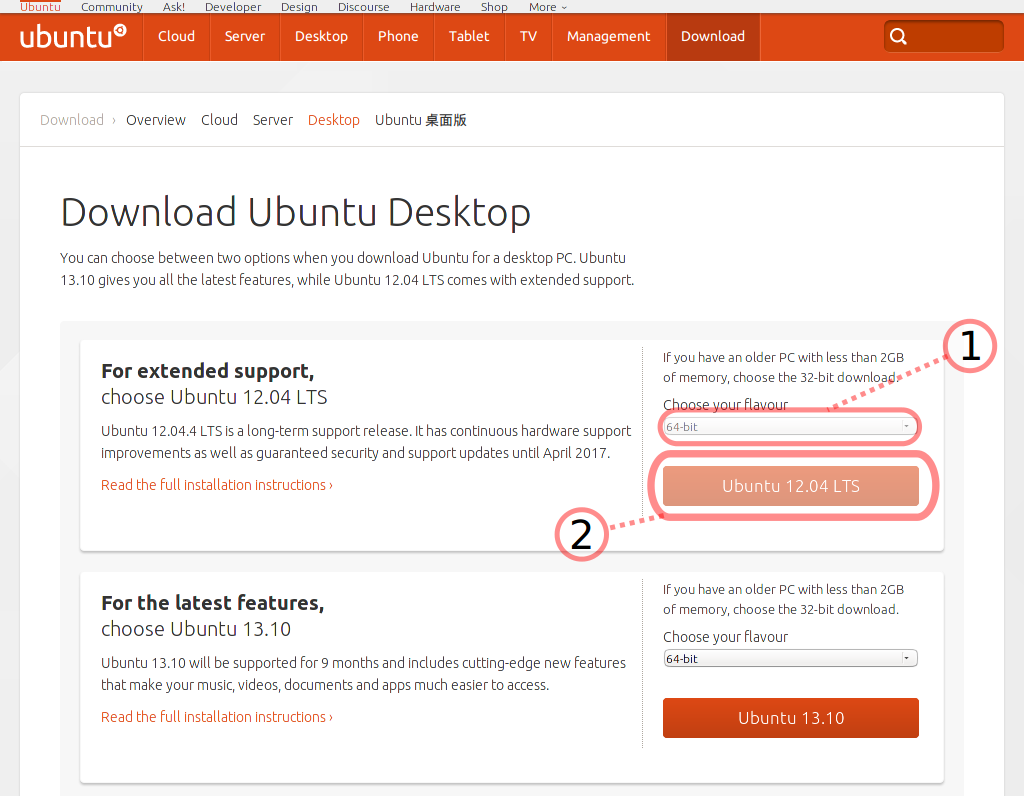
\includegraphics[width=\linewidth]{images/instalacja_pobieranie_obrazu.png}
\end{center}

Pierwszym etapem instalacji systemu jest pobranie instalatora. W tym celu udaj się na stronę \href{http://www.ubuntu.com/download/desktop}{ubuntu.com} i z górnego paska wybierz \textcolor{ubuntu_orange}{Download} a następnie \textcolor{ubuntu_orange}{Desktop}
\begin{enumerate}[label=\protect\circled{\arabic*}]
\item To pole pozwali ci wybrać pomiędzy 32- a 64-bitową wersją systemu. Domyślnie wybrana jest opcja 64 bitowa.
\item Kliknij na ten przycisk aby przejść dalej.
\end{enumerate}

Na kolejnym ekranie będziesz mieć możliwość przekazania dotacji na rzecz Ubuntu. W tym momencie nas to nie interesuje. Przesuń stronę w dół i kliknij na \textcolor{ubuntu_orange}{Not now, take me to the download}. Zostaniesz przeniesiony na kolejną stronę, a po kilku sekundach rozpocznie się pobieranie obrazu systemu.

Jeżeli twój komputer został wyprodukowany nie dawnej niż 5 lat temu, wersja 64-bitowa będzie na pewno odpowiednia. Jeżeli masz mniej niż 2 GB RAM-u, wybierz wariant 32-bitowy. Niezależnie od tego jaką wersję wybierzesz, i tak będziesz mieć dostęp do takiego samego zestawu oprogramowania. Wariant 64-bitowy jest lepiej dopasowany do nowoczesnych systemów, jeżeli jednak masz jakiekolwiek wątpliwości, wybierz wersję 32-bitową. Będzie ona działać także na 64-bitowym komputerze, choć nie będzie wykorzystywać wszystkich jego możliwości.
Jeżeli twoja płyta główna kontrolowana jest przez UEFI, musisz wybrać system 64-bitowy.
Linki do pobierania bezpośredniego:
\begin{itemize}
\item \href{http://www.ubuntu.com/start-download?distro=desktop&bits=64&release=lts}{Wersja 64 bitowa (733 megabajtów).}
\item \href{http://www.ubuntu.com/start-download?distro=desktop&bits=32&release=lts}{Wersja 32 bitowa (731 megabajtów).}
\end{itemize}
        \subsection{Nagrywanie pobranego obrazu}
                Po zakończeniu pobierania obrazu instalatora należy nagrać go na zewnętrzny nośnik i uruchomić komputer z tego nośnika. Najlepszym rozwiązaniem jest użycie klucza usb (pendriva), gdyż obrazy instalacyjne Ubuntu są zbyt duże aby zmiejścić się na krążkach CD. Jednak nie wszystkie komputery potrafią startować z klucza USB. Jeżeli twój komputer nie ma takiej właściwości, będziesz musiał użyć płyty DVD lub karty (micro)SD.
\subsubsection{System Windows, nagrywanie na pendriva}
\begin{wrapfigure}{r}{0.5\textwidth}
		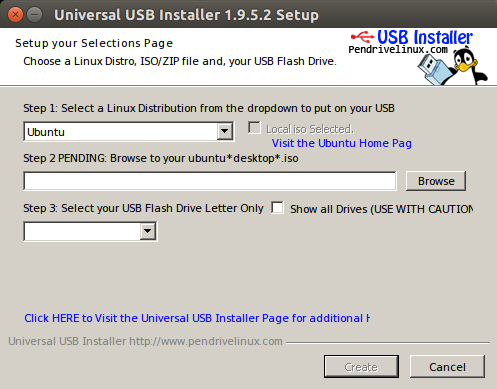
\includegraphics[width=\linewidth]{images/instalacja_nagrywanie_obrazu.png}
\end{wrapfigure}
\noindent Jeżeli chcesz użyć pendriva jako nośnika instalacyjnego to upewnij się iż ma on przynajmniej 1 gigabajt pojemności. W przeciwnym wypadku instalator nie zmiejści na nim. Jeżeli masz już przygotowany pendrive, wykonaj co następuje:
\begin{enumerate}
%TODO dla tej listy użyć włąsnych znaczników (label) przypominających te użyte na obrazkach.
\item Pobierz program \href{http://www.pendrivelinux.com/downloads/Universal-USB-Installer/Universal-USB-Installer-1.9.5.2.exe}{Universal USB Installer}.
\item Uruchom pobrany plik.
\item Zaakecptuj umowę licencyjną.
\item Podłącz do komputera pendrive, który ma użyty jako nośnik.
\item Z tej listy wybierz Ubuntu.
\item Kliknij na przycisk Browse i wskaż pobrany wcześniej obraz instalatora Ubuntu.
\item Z tej listy wybierz wczesniej podłączony pendrive.\\
\textbf{UWAGA: Wszystkie dane na nim zostaną skasowane!}
\item Kliknij przycisk CREATE.
\item Poczekaj na zakończenie operacji.
\end{enumerate}
\clearpage
\subsubsection{System Windows 7 / 8, nagrywanie na płytę DVD}
%TODO zweryfikować, czy windows 8 też to ma
\begin{wrapfigure}{r}{0.5\textwidth}
		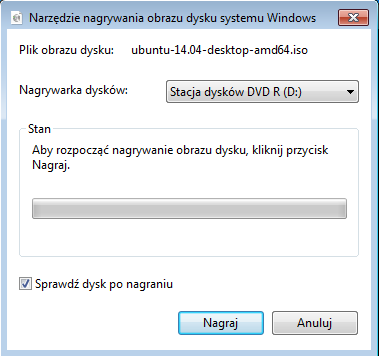
\includegraphics[width=\linewidth]{images/instalacja_nagrywanie_obrazu_DVD.png}
\end{wrapfigure}
Systemy operacyjne Windows 7 i 8 mają wbudowane narzędzie do wypalania plików .iso na płytach. Kliknij prawym przyciskiem myszy na pobrany obraz instalatora Ubuntu, wybierz opcję "Otwórz w" a następnie "Windows Disc Image Burner".
\begin{enumerate}
%TODO dla tej listy użyć włąsnych znaczników (label) przypominających te użyte na obrazkach.
%TODO jak to się po polsku nazywa?
\item Z tej listy wybierz swoją nagrywarkę.
\item Włóż czystą płytę DVD na wybranego napędu.
\item Upewnij się, że zaznaczone jest pole "Zweryfikuj dysk po nagraniu"
\item Kliknij na przycisk \textbf{Nagraj}
\end{enumerate}
\clearpage
\subsubsection{System Windows XP i inne starsze wersje, nagrywanie na płytę DVD}
\begin{wrapfigure}{R}{0.5\linewidth}
		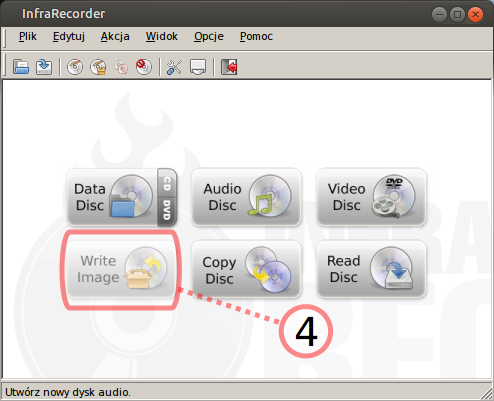
\includegraphics[width=\linewidth]{images/instalacja_nagrywanie_obrazu_DVD_winXP.png}
\end{wrapfigure}
Starsze wersje systemu Windows nie mają wbudowanej możliwości nagrywania płyt DVD. Potrzebne będzie do tego osobne narzędzie, program służący do wypalania płyt. Obsługa tych programów jest bardzo podobna: należy wybrać opcję \emph{Nagrywanie obrazu na płytę}. Koniecznie nagrywaj z wykorzystaniem tej opcji, gdyż inne (np.\emph{Nagrywanie płyty z danymi} lub \emph{Tworzenie kopi zapasowej}) utworzy dysk, którego twój komputer nie będzie potem wstanie uruchomić. Dla przykładu posłużymy się programem Infra Recorder.

\begin{enumerate}
\item Pobierz i zainstaluj program \href{http://infrarecorder.org/?page_id=5}{Infra Recorder}.
\item Uruchom nowozainstalowany program.
\item Włóż czystą płytę DVD do nagrywarki.
\item W programie Infra Recorder wybierz opcję \textbf{Write Image}.
\item Wybierz pobrany wcześniej obraz instalatora Ubuntu.
\item Kliknij na przycisk \textbf{OK}.
\end{enumerate}
\clearpage











                \subsubsection{System Linux, nagrywanie na pendriva}
\begin{wrapfigure}[6]{r}{0.5\textwidth}
                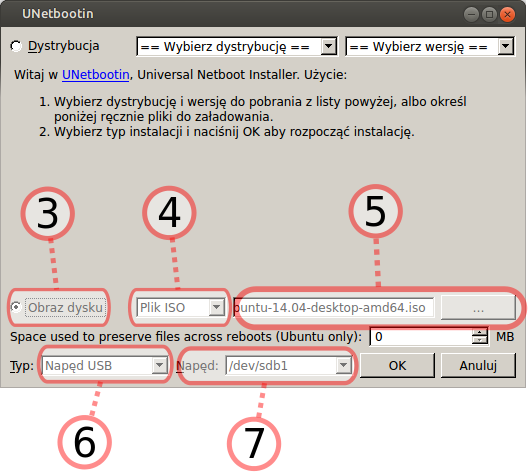
\includegraphics[width=\linewidth]{images/instalacja_nagrywanie_obrazu_linux.png}
\end{wrapfigure}

W systemach operacyjnych Linux do nagrywania obrazu na pendrive'a najlepiej posłużyć się programem \textcolor{ubuntu_orange}{UNetbootin}, dostępnym w każdej dystrybucji. Podłącz do komputera klucz USB, z którego chcesz potem instalować Ubuntu.
\begin{enumerate}[label=\protect\circled{\arabic*}]
\item Zainstaluj UNetBootIn korzystając ze swojego menadżera pakietów.
\item Uruchom zainstalowany przed momentem program.
\item Zaznacz pole Obraz dysku
\item Z menu wybierz Plik ISO
\item W tym polu podaj ścieżkę do pobranego wcześniej obrazu instalatora Ubuntu. Wciśnij przycisk oznaczony trzema kropkami (“\ldots”) i wskaż plik.
\item W tym menu wybierz Napęd USB
\item Z tego menu wybierz podłączonego wcześniej pendriva.\\
\textbf{UWAGA: Wszystkie dane znajdujące się na tym nośniku zostaną skasowane!}
\item Kliknij przycisk OK aby rozpocząć nagrywanie
\end{enumerate}
\subsubsection{System Linux, nagrywanie na DVD}
%TODO potrzebny obrazek z włożoną płytą DVD i wybranym obrazem ubuntu 14.04
\begin{wrapfigure}{l}{0.5\textwidth}
                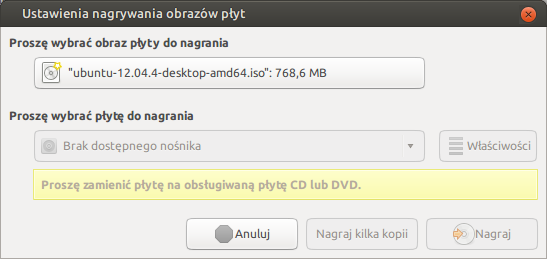
\includegraphics[width=\linewidth]{images/instalacja_nagrywanie_obrazu_linux_DVD.png}
\end{wrapfigure}

Aby nagrać obraz na płytę DVD potrzebujesz odpowiedniego programu. W tym przykładzie posłużymy się dostępną w większości dystrybucji nagrywarką Brasero. Kliknij prawym przyciskiem myszy na pobrany wcześniej obraz instalatora Ubuntu, wybierz \textcolor{ubuntu_orange}{Otwórz w\ldots}, a następnie wybierz \textcolor{ubuntu_orange}{Brasero}. W otwartym oknie zostaniesz poproszony o włożenie czystej płyty DVD. Zrób to, a następnie kliknij na przycisk \textcolor{ubuntu_orange}{Nagraj}.
\clearpage

        \subsection{Przygotowanie do instalacji}
                \subsubsection{Przygotowanie do instalacji - Windows - wskazówki ogólne}
\label{sec:przygotowanie_windows}
Instalując inny system operacyjny na dysku twardym swojego komputera zawsze istnieje ryzyko utraty danych. Wiele rzeczy może się zdażyć. Utrata zasilania w czasie partycjonowania dysku twardego najczęściej prowadzi do utraty jesgo zawartości. Przez zwykłą nieuwagę można nadpisać jede system drugim i w ten sposób utracić dane. Dlatego nim przystąpisz do instalacji systemu ubuntu upewnij się iż wszystkie wazne dane zostały zabezpieczone na zewnętrznych nośnikach danych. Innymi słowy: zrób kopię zapasową.

Warto też wyeksportować dane z programów takich jak przeglądarka internetowa(zakładki), klient pocztowy(konta, kalendarze i kontakty) i komunikator internetowy(konta, historia rozmów, znajomi). Nie zapomniej zrobić kopi zapasowej dokumentów czy swojej kolekcji muzyki. Jeżeli zainstalujesz Ubuntu obok Windowsa, to będziesz mieć dostęp do swoich plików. Niestety, w drugą stronę to nie działa i na systemach Windows nie ma możliwości podglądu plików na partycjach systemów Linuksowych\footnote{To jest możliwe, ale dosyć skomplikowane i wykracza poza zakres tego przewodnika}.

Ważnym krokiem jest ustalenie czy twoja płyta główna obsługiwana jest przez UEFI i jeżeli tak to jakie opcje są włączone. W konsoli systemu Windows (Start $\rightarrow$ Uruchom $\rightarrow$ cmd) wpisz \textit{Confirm-SecureBootUEFI}. System może zwrócić jedną z trzech informacji:
\begin{itemize}
\item \textit{Cmdlet not supported on this platform} lub \textit{Polecenia nie znaleziono} - Ten komputer nie korzysta z SecureBoot. Nie potrzebujesz nic więcej robić, wystarczy włożyć przygotowany nośnik instalacyjny i zainstalowac Ubuntu.
\item \textit{False} - Ten komputer na UEFI, ale nie korzysta z SecureBoot. Przejdź do sekcji porad dla Windows 8
\item \textit{True} - Ten komputer na UEFI, ale korzysta z SecureBoot. Przejdź do sekcji porad dla Windows 8
\end{itemize}
\subsubsection{Przygotowanie do instalacji - Windows 8}
\label{sec:przygotowanie_windows8}
Windows 8 wymusił na producentach sprzetu stosowanie technologi UEFI (zamiast BIOSu) oraz SecureBoot(Zabezpieczenie komputera przed zmianami systemu operacyjnego), co znacznie utrudniło instalację innych systemów operacyjnych. Ubuntu jest przygotowane do współpracy z Windowsem 8, ale Windows nie jest przygotowany do współdzielenia komputera z innymi systemami operacyjnymi. Pamiętaj, że jeżeli posiadasz UEFI (a używanie Windows 8 na to wskazuje) to potrzebujesz Ubuntu w wersji 64 bitowej. Systemy 32 bitowe nie są obsługiwane przez technologię UEFI\footnote{A przynajmniej nie bez dużej ilości kombinowania}.

W tym momencie warto przygotować wolną przestrzeń na dysku pod instalację Ubuntu. Ten punkt można wykonać zarówno teraz jak i podczas instalacji Ubuntu, jednak jeżeli używasz Windows 8 lepiej zrobić to teraz. Wciśnij kombinację klawiszy super + r i uruchom program compmgmt.msc. W uruchomionym programie utwórz partycję dla Ubuntu. Absolutne minimum dla tej partycji to 8 gigabajtów. Ubuntu potrzebuje około 4 gigabajtów na podstawową instalację, pozostałe miejsce będzie można przeznaczyć na instalację oprogramowania oraz pliki uzytkownika. Zalecamy jednak stworzneie przynajmniej 20 gigabajtowej partycji.

Windows 8 korzysta z opcji Szybkiego Uruchamiania (Fast Boot), która to uniemożliwia dostęp do plików Windowsa przez system Ubuntu. Jedynym sposobem na obejście tego jest wyłączenie opcji Szybkiego uruchamiania. Wejdź w Panel Sterowania, następnie Opcje Zasilania a potem Wybierz co ma robić przycisk zasilania. Odhacz opcję "Włącz Szybkie uruchamiania (zalecane)".

\subsubsection{Przygotowanie do instalacji - Linux}
\label{sec:przygotowanie_linux}
Instalacja jednego systemu Linux obok drugiego nie powoduje zadnych problemów, jednak powinieneś wiedzieć o paru sprawa. W Linuksach pliki użytkownika są przechowywane w katalogu /home. Dobrą praktyką jest wydzielenie osobnej partycji dla tego katalogu, aby przy reinstalacji systemu nie tracić swoich ustawień. Jeżeli instalujesz jednego Linuksa obok drugiego to kuszącym może być wykorzystanie jednej partycji domowej dla obu systemów. 
To jest możliwe, ale weź pod uwagę iż różne systemy mogą korzystać z różnych plików - nie wszystkie ustawienia będą widoczne na obu systemach (szczególnie jeżeli korzystasz z różnych środowisk graficznych). Przy takiej konfiguracji ważne jest też aby nazwa użytkownika oraz jego grupy były taka sama na obu systemach.
Jeżeli systemy, które instalujesz obok siebie bardzo się różnią, to lepiej nie korzystać ze wspólnego katalogu domowego, a ze wspólnych dokumentów, filmów czy muzyki korzystać za pomocą wspólnego katalogu.

Potrzebujesz tylko jednej partycji wymiany (swap) niezależnie od tego ile systemów instalujesz.
        \subsection{Uruchomienie instalatora}
                \subsubsection{Ponowne uruchomienie komputera}
Jeżeli dysponujesz już  nośnikiem instalacyjnym, nie pozostaje nic innego, jak uruchomić instalator i zainstalować system na dysku twardym komputera. Jeśli korzystasz z tego przewodnika w trybie online, dobrym pomysłem będzie wydrukowanie kilku kolejnych stron. Może się zdarzyć, że w czasie instalacji stracisz dostęp do internetu i zostaniesz tym samym odcięty od zawartych tutaj informacji.

Przed przystąpieniem do instalacji koniecznie zapoznaj się także z następującymi sekcjami:
\begin{itemize}
\item \ref{sec:przygotowanie_windows} \textit{Przygotowanie do instalacji - Windows - wskazówki ogólne}: ta sekcja zawiera przydatne informacje dla osób migrujących z systemów Windows.
\item \ref{sec:przygotowanie_windows8} \textit{Przygotowanie do instalacji - Windows 8}: pecyficzne porady dla systemu Windows 8. Koniecznie ten fragment przewodnika, jeżeli instalujesz Ubuntu obok Windows 8 lub próbujesz zainstalować Ubuntu zamiast Windows 8.
\item \ref{sec:przygotowanie_linux} \textit{Przygotowanie do instalacji - Linux}: ogólne wskazówki dla osób instalujących Ubuntu obok innych dystrybucji Linuksa.
\end{itemize}
Zrestartuj swój komputer i uruchom go z przygotowanego nośnika instalacyjnego. W większości przypadków wiąże się to z ręcznym wskazaniem odpowiedniego napędu podczas uruchamiania komputera. Jeśli twój komputer wyposażony jest w system UEFI, cała ta procedura będzie znacznie bardziej skomplikowana.

\subsubsection{Zmiana kolejności bootowania}
Kiedy rozpocznie się rozruch komputera, jeszcze przed załadowaniem się systemu operacyjnego musisz poinformować maszynę, że tym razem  zamiast systemu zainstalowanego na twardym dysku ma ona wykorzystać przygotowany przez nas instalator. Każdy producent płyt głównych podchodzi do tej kwestii w nieco odmienny sposób, jednak najczęściej procedura będzie się pokrywać z jednym z opisanych poniżej scenariuszy:
\begin{itemize}
\item Niektóre komputery podczas rozruchu pokazują napis Press F12 to select boot device. Kluczowymi słowami są tutaj ”Boot Device”, ”Boot order” lub podobne . Wciśnij wskazany klawisz (w tym konkretnym przypadku F12, ale nie jest to reguła) i z wyświetlonego menu wybierz nośnik instalacyjny. Niektóre komputery wykrywają pendrive'y jako dyski twarde i musisz wskazać właśnie taki dysk twardy a nie port USB. Jeżeli na liście nie ma naszego instalatora, zresetuj komputer i spróbuj ponowanie.
\item Jeżeli zobaczysz napis \textbf{Press ESC to enter setup} lub coś podobnego, twoim słowem kluczowym będzie ”setup”. Wciśnięcie odpowiedniego klawisza (ESC, delete lub któryś z klawiszy funkcyjnych) spowoduje uruchomienie programu konfiguracyjnego płyty głównej. W tym programie przejdź do sekcji ”Advanced BIOS Features” a następnie ”First Boot Device”. Wskaż napęd CD-ROM lub napęd USB (względnie drugi dysk twardy, jeżeli pendrive jest rozpoznawany jako dysk twardy). Wróć do menu głównego (klawisz ESC cofa o jedno menu) i zapisz zmainy (najczęściej F10, czasem ESC i potwierdzenie przy pomocy klawisza Y). W tym momencie komputer samoczynnie się zrestartuje.
\end{itemize}
\subsubsection{Uruchomienie instalatora UEFI}
Po wybraniu urządzenia z nośnikiem instalacyjnym komputer rozpocznie proces jego uruchamiania. Może to potrwać od kilku do kilkunastu sekund. W tym czasie ekran komputera będzie czarny bądź będą się przez niego przewijały napisy.\\
Jeżeli twoja maszyna pracuje pod kontrolą UEFI, to pierwszy ekran instalatora będzie wyglądał jak na poniższym rysunku:
\begin{center}
	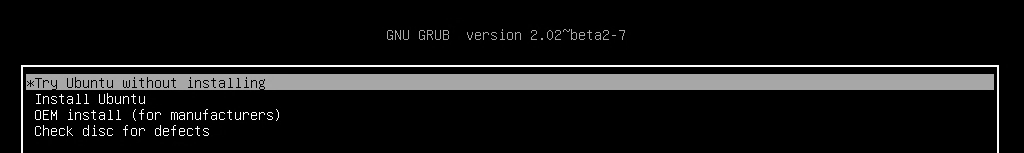
\includegraphics[width=\linewidth]{images/instalacja_UEFI_boot.png}
\end{center}
Do wyboru masz następujące opcje:
\begin{description}
\item[Try Ubuntu without installing](Wypróbuj Ubuntu bez instalowania) - Uruchomi system Ubuntu bez instalacji go na dysku twardym. W ten sposób możesz przetestować Ubuntu i zobaczyć jak działa w praktyce. Wszystkie zmiany jakie wprowadzisz w systemie zostaną odrzucone po wyłączeniu komputera. Należy pamiętać, że w tym trybie Ubuntu działa bardzo wolno, gdyż musi korzystać z powolnego nośnika (płyta DVD lub pendriva). Po normalniej instalacji ubuntu będzie działać z pełną wydajnością. Skrót do instalatora systemu znajduje się na Pulpicie.
\item[Install Ubuntu](Zainstaluj Ubuntu) - Ta opcja bezpośrednio uruchomi instalator Ubuntu bez wczytywania całego systemu.
\item[OEM Install](Instalacja dla producentów sprzętu) - Ta opcja pozwala zainstalować podstawowy system bez tworzenia użytkownika. Przy pierwszym uruchomieniu zostaniesz poproszony o stworzenie nowego użytkownika.
\item[Check disk for defects](Sprawdź płytę pod kontem błędów odczytu) - Ta opcja sprawdzi czy używany nośnik został prawidłowo utworzony.\\
Przed przystąpieniem do instalacji systemu warto wykonać sprawdzenie nośnika instalacyjnego. Potrwa to góra kilka minut a pozwoli zaoszczędzić czas w przyszłości. Podczas przeprowadzania testów komputer może wyświetlać tylko czarny ekran. Jeżeli nie znajdzie żadnych błędów, otrzymasz komunikat "Check Finished: No errors found. Press any key to reboot your system" (Zakończono sprawdzanie: Nie znaleziono błędów.Wciśnij dowolny klawisz aby zresetować komputer). Po ponownym uruchomieniu komputera możesz przystąpić do instalacji. Jeżeli znaleziono jakiekolwiek błędy to należy ponownie przygotować nośnik instalacyjny. Uzycie wadliwego instalatora doprowadzi do uszkodzenia systemu. 
\end{description}

\subsubsection{Uruchomienie instalatora BIOS}
\begin{wrapfigure}{L}{0.4\textwidth}
		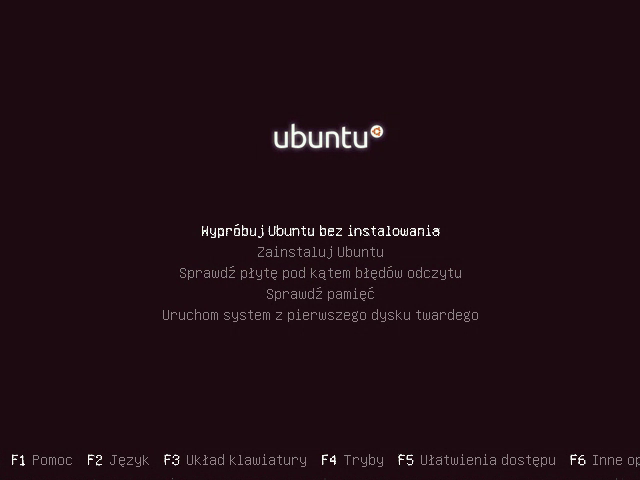
\includegraphics[scale=0.5]{images/instalacja_BIOS_boot.png}
\end{wrapfigure}
Po wybraniu urządzenia z nośnikiem instalacyjnym komputer rozpocznie proces jego uruchamiania. Może to potrwać od kilku do kilkunastu sekund. W tym czasie ekran komputera będzie czarny bądź będą się przez niego przewijały napisy. Kiedy ekran komputera zmieni kolor z czarnego na fioletowy wciśnij dowolny klawisz aby wejść do ustawień instalatora. Jeżeli tego nie zrobisz, komputer uruchomi instalator z domyślnymi opcjami.Na początek wybierz język w jakim system bedzie się z toba komunikował. Przy pomocy klawiszy kursora przejdź do trzeciej kolumny. Język Polski  znajduje się mniej więcej w połowie tej kolumny. Wciśnij enter aby zatwierdzić.
\clearpage
\begin{description}
\item[Wypróbuj Ubuntu bez instalowania] - Uruchomi system Ubuntu bez instalacji go na dysku twardym. W ten sposób możesz przetestować Ubuntu i zobaczyć jak działa w praktyce. Wszystkie zmiany jakie wprowadzisz w systemie zostaną odrzucone po wyłączeniu komputera. Należy pamiętać, że w tym trybie Ubuntu działa bardzo wolno, gdyż musi korzystać z powolnego nośnika (płyta DVD lub pendriva). Po normalniej instalacji ubuntu będzie działać z pełną wydajnością. Skrót do instalatora systemu znajduje się na Pulpicie.
\item[Zainstaluj Ubuntu] - Ta opcja bezpośrednio uruchomi instalator Ubuntu bez wczytywania całego systemu.
\item[Sprawdź płytę pod kontem błędów odczytu] - Ta opcja sprawdzi czy używany nośnik został prawidłowo utworzony.\\
Przed przystąpieniem do instalacji systemu warto wykonać sprawdzenie nośnika instalacyjnego. Potrwa to góra kilka minut a pozwoli zaoszczędzić czas w przyszłości. Podczas przeprowadzania testów komputer może wyświetlać tylko czarny ekran. Jeżeli nie znajdzie żadnych błędów, otrzymasz komunikat "Check Finished: No errors found. Press any key to reboot your system" (Zakończono sprawdzanie: Nie znaleziono błędów.Wciśnij dowolny klawisz aby zresetować komputer). Po ponownym uruchomieniu komputera możesz przystąpić do instalacji. Jeżeli znaleziono jakiekolwiek błędy to należy ponownie przygotować nośnik instalacyjny. Uzycie wadliwego instalatora doprowadzi do uszkodzenia systemu. 
\item[Sprawdź pamięć] - Ta opcja uruchomi program memtest, który wykona test pamięci operacyjnej komputera (RAM). Uszkodzona pamięć jest jedną z częstrzych przyczyn błędów instalatora jak i wpływa negatywnie na pracę zainstalowanego systemu.
\item[Uruchom system z pierwszego dysku twardego] - Ta opcja kończy pracę instalatora i uruchamia podstawowy system operacyjny komputera.
\end{description}
Dodatkowe opcje widoczne na dolnym pasku uruchamia się wciskając odpowiedni klawisz funkcyjny:
\begin{description}
\item[F1] - Wyświetla pomoc, wraz z szczegółowym opisem poszczególnych opcji konfiguracyjnych.
\item[F2] - Zmiana języka instalatora.
\item[F3] - Zmiana układu klawiatury.
\item[F4] - Zmiana trybu pracy instalatora.
	\begin{description}
	\item[Zwykły] - Tryb podstawowy, teraz się w nim znajdujesz
	\item[Użycie nośnika aktualizującego sterowniki] - ??
	\item[Instalacja OEM(dla producentów sprzętu)] - Ta opcja pozwala zainstalować podstawowy system bez tworzenia użytkownika. Przy pierwszym uruchomieniu zostaniesz poproszony o stworzenie nowego użytkownika.
	\end{description}
\item[F5] - Pozwala włączyć/wyłączyć dodatkowe opcje ułatwiające instalacje osobom niepełnosprawny (Klawiatura ekranowa, lupa, wyski kontrast, czytnik ekranu, klawiatura Braille'a)
\item[F6] - Dodatkowe parametry rozruchu, pomocne w przypadku napotkania problemów ze sprzetem.
\end{description}
\clearpage


        \subsection{Graficzny instalator Ubuntu}
                Niezależnie od tego, czy posiadasz płytę główną z BIOS-em, czy z UEFI, w poprzednim punkcie powinieneś wybrać \textcolor{ubuntu_orange}{Zainstaluj Ubuntu}. Ta metoda jest szybsza od \textcolor{ubuntu_orange}{Wypróbuj Ubuntu bez instalowania}, gdyż nie wymaga załadowania całego systemu. Jeżeli mimo wszystko uruchomiłeś cały system w trybie Live, to na pulpicie znajdziesz ikonę \textcolor{ubuntu_orange}{Zainstaluj Ubuntu} (lub ,,Install Ubuntu'', jeżeli nie zmieniałeś języka). Od tego momentu instalacja przebiega w identyczny sposób dla każdego wybranego sposobu instalacji.

W czasie instalacji w prawej części paska u góry ekranu znajduje się szerego ikon:
\begin{description}
\item[
\includegraphics{images/ikony_dostempnosc.png}]\textcolor{ubuntu_orange}{Dostępność} --- uruchomienie lupy, czytnika ekranowego lub klawiatury ekranowej.
\item[
\includegraphics{images/ikony_internet.png}]\textcolor{ubuntu_orange}{Łączność} --- konfiguracja połączenia z internetem na czas instalacji systemu.
\item[
\includegraphics{images/ikony_jezyk.png}]\textcolor{ubuntu_orange}{Język} --- zmiana języka oraz układu klawiatury na czas instalacji systemu.
\item[
\includegraphics{images/ikony_dzwiek.png}]\textcolor{ubuntu_orange}{Ustawienia głośności i dźwięku}
\item[
\includegraphics{images/ikony_zasilanie.png}]\textcolor{ubuntu_orange}{Zasilanie} --- wyłączenie lub ponowne uruchomienie komputera.
\end{description}
\clearpage
\subsubsection{Wybór języka}
\begin{center}
        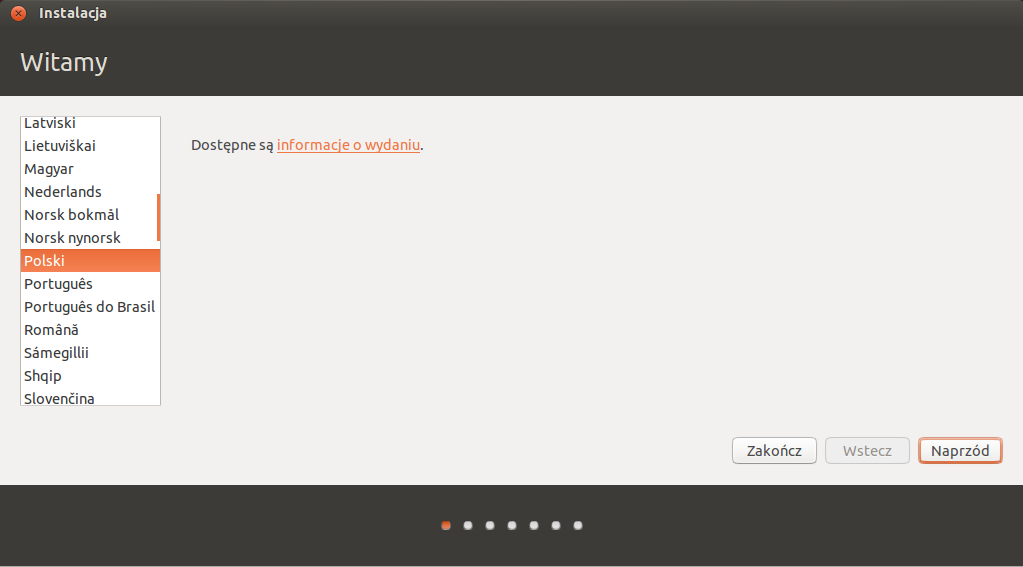
\includegraphics[width=\linewidth]{images/instalator_jezyk.png}
\end{center}

Pierwszy ekran instalatora pozwala wybrać język. Jeżeli wcześniej nie zmieniłeś języka na polski, to teraz masz ku temu okazję. Język wybrany podczas instalacji będzie także domyślnym językiem zainstalowanym w systemie.
\begin{flushright}
Kliknij przycisk \textcolor{ubuntu_orange}{Naprzód}, aby przejść dalej.
\end{flushright}
\clearpage
\subsubsection{Konfiguracja Wi-Fi}
\begin{center}
        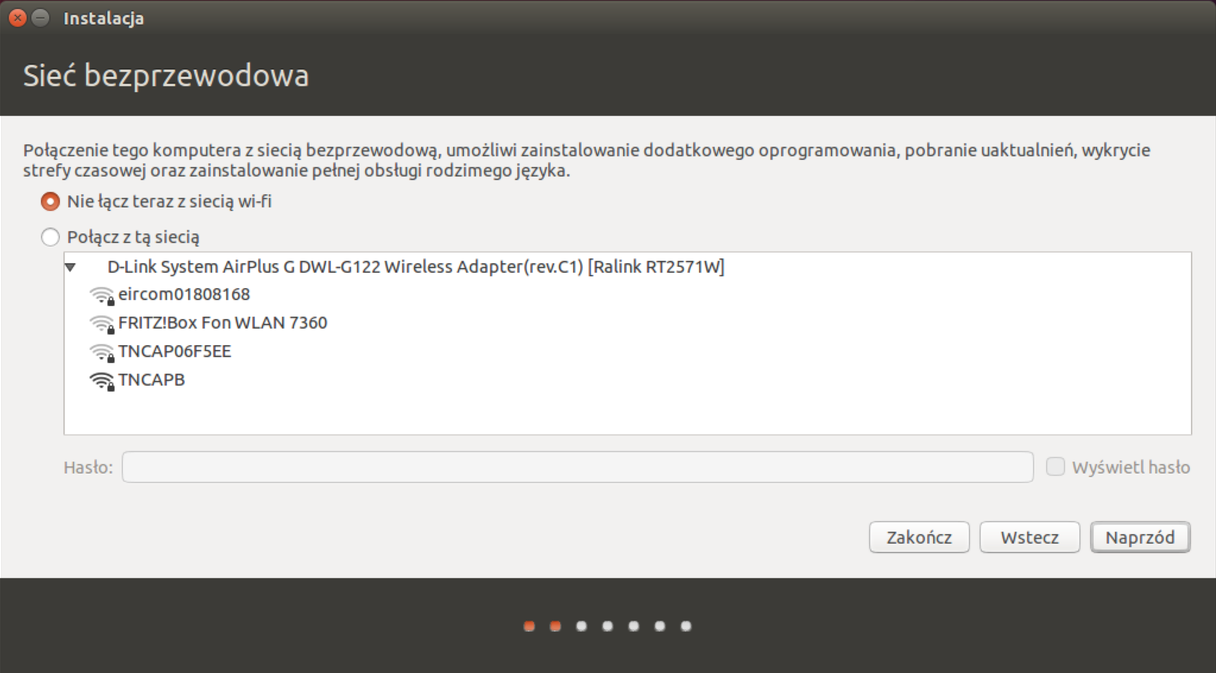
\includegraphics[width=\linewidth]{images/instalator_wifi.png}
\end{center}

Drugi ekran instalatora pozwala skonfigurować połączenie bezprzewodowe Wi-Fi. Jeżeli instalator nie wykryje żadnej karty Wi-Fi, to nie pokaże tego ekranu. Ten etap instalacji zostanie pominięty również wtedy, gdy uda się nawiązać połączenie przewodowe.

Z listy na ekranie wybierz sieć bezprzewodową, z którą chcesz się połączyć. Wpisz hasło do sieci bezprzewodowej w pole \textcolor{ubuntu_orange}{Hasło}.
\begin{flushright}
Kliknij przycisk \textcolor{ubuntu_orange}{Naprzód}, aby przejść dalej.
\end{flushright}
\clearpage
\subsubsection{Sprawdzenie kompatybilności sprzętu, wybór dodatkowych komponentów}
\begin{center}
        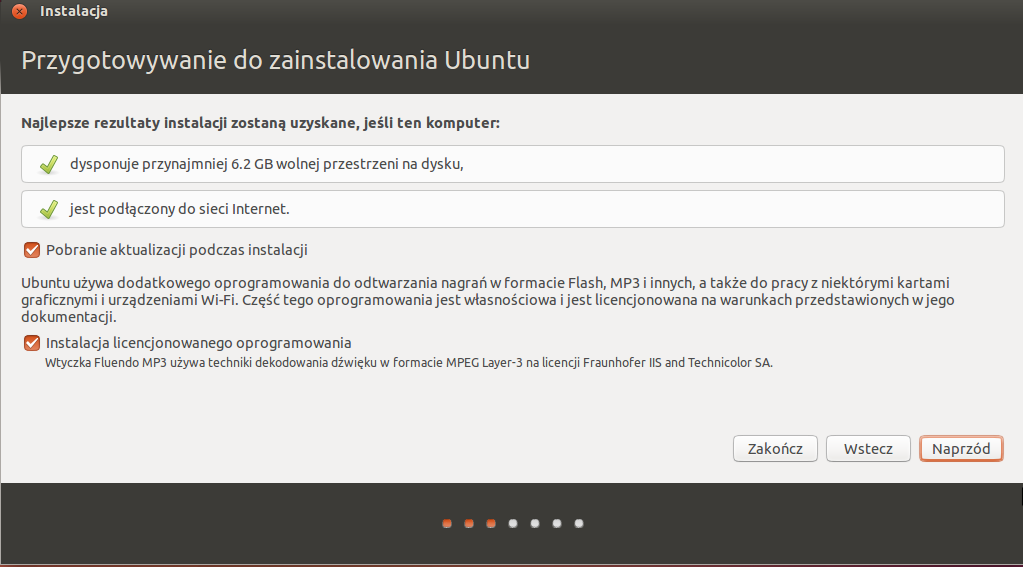
\includegraphics[width=\linewidth]{images/instalator_wymagania.png}
\end{center}

Na tym etapie instalator sprawdzi, czy na dysku twardym jest wystarczająco dużo miejsca, aby zainstalować Ubuntu. Połączenie z internetem nie jest wymagane do zainstalowania systemu, jest jednak niezbędne, by zainstalować spolszczenie, aktualizacje oraz dodatkowe wtyczki. Jeżeli w tym momencie nie masz połączenia z internetem, to pobranie paczek lokalizacyjnych będzie możliwe później. Zostało to opisane w rozdziale \ref{rzeczy_do_zrobienia_po_instalacji} ,,Rzeczy do zrobienia po instalacji Ubuntu''.
\begin{itemize}
\item \textcolor{ubuntu_orange}{Pobieranie aktualizacji podczas instalacji} --- Instalator pobierze i zainstaluje wszystkie aktualizacje, które zostały wydane od dnia premiery systemu.
\item \textcolor{ubuntu_orange}{Instalacja licencjonowanego oprogramowania} --- W skład pakietu wchodzą własnościowe sterowniki do kart graficznych AMD lub Nvidii, sterowniki do kart Wi-Fi, kodeki audio-wideo (po instalacji Ubuntu będzie w stanie odtworzyć prawie każdy rodzaj plików muzycznych i filmowych) oraz wtyczka Flash do przeglądarki internetowej.
\end{itemize}
\begin{flushright}
Kliknij przycisk \textcolor{ubuntu_orange}{Naprzód}, aby przejść dalej.
\end{flushright}
\clearpage
\subsubsection{Partycjonowanie dysku twardego}
\begin{center}
        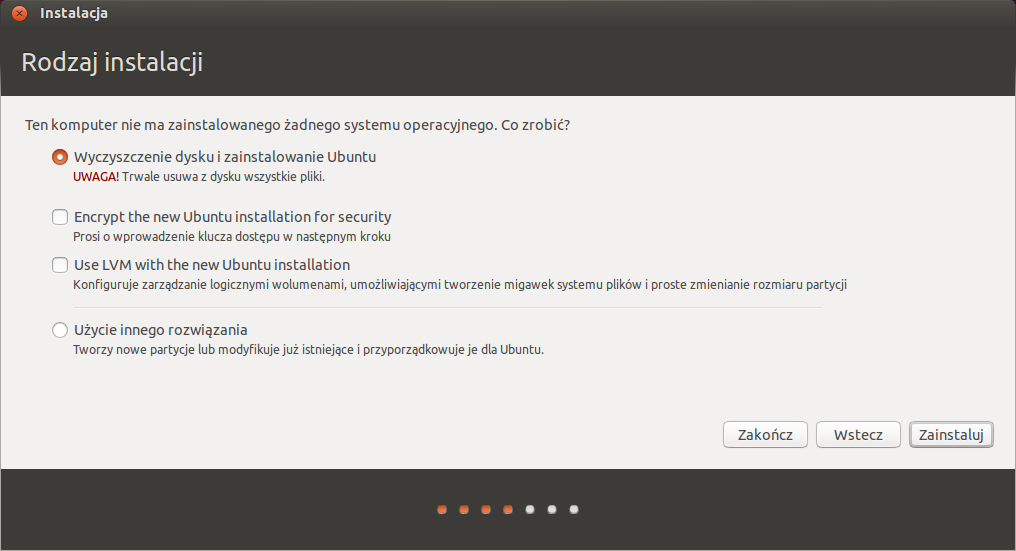
\includegraphics[width=\linewidth]{images/instalator_partycjonowanie_proste.png}
\end{center}

Jest to najważniejszy etap instalacji. W tym miejscu można dokonać cudów, jak i zniszczyć cały dysk twardy. Jako że prawidłowe partycjonowanie dysku twardego to bardzo szeroki temat, to poświęciliśmy mu cały osobny rozdział. Na powyższym obrazie widać najprostszą wersję tego etapu instalacji. Na dysku twardym nie ma zainstalowanego żadnego systemu operacyjnego i instalator proponuje wykorzystanie całej przestrzeni dla Ubuntu. Jeżeli masz inne systemy operacyjne, to instalator zaproponuje wydzielenie miejsca i instalację Ubuntu obok danego systemu operacyjnego. Jeżeli miałeś wcześniej zainstalowane Ubuntu, instalator zaproponuje aktualizację do najnowszego wydania lub usunięcie i zainstalowanie Ubuntu ponownie.
Partycjonowanie zostało szeroko opisane w rozdziale \ref{subsec:partycjonowanie} ,,Zaawansowane partycjonowanie''. Wróć tutaj, gdy go przeczytasz.
\begin{flushright}
Kliknij przycisk \textcolor{ubuntu_orange}{Naprzód}, aby przejść dalej.
\end{flushright}
\clearpage
\subsubsection{Wybór strefy czasowej}
\label{instalator_strefa_czasowa}
\begin{center}
        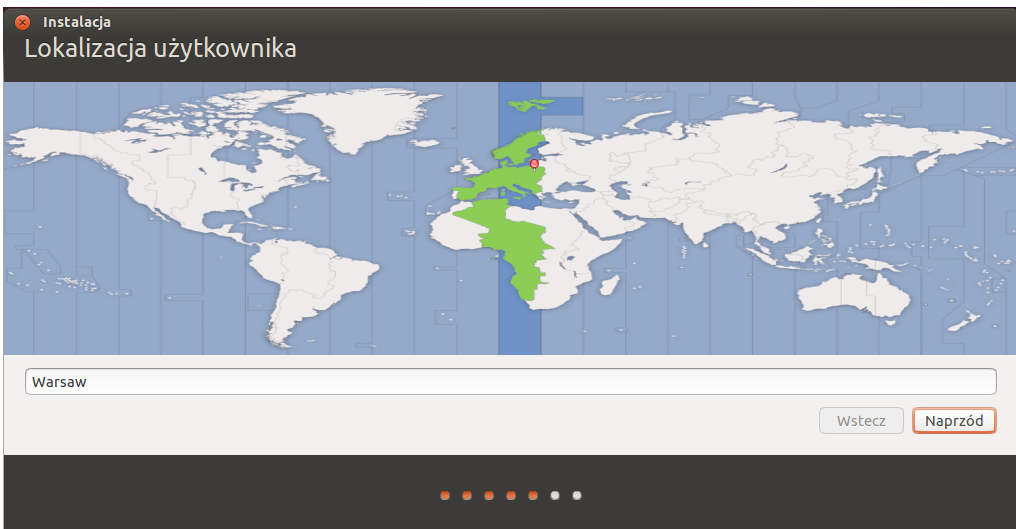
\includegraphics[width=\linewidth]{images/instalator_czas.png}
\end{center}

Na tym etapie należy wybrać lokalizację tego komputera, aby system mógł wyświetlać prawidłowy czas i automatycznie dostosowywać się do zmian pomiędzy czasem letnim i zimowym. Jeżeli w trakcie instalacji masz połączenie z internetem, to odpowiednia lokalizacja zostanie wybrana automatycznie. Jeżeli nie masz dostępu do internetu, w pole wpisz \textcolor{ubuntu_orange}{Warsaw}. Stolica naszego kraju określa też naszą strefę czasową.
\begin{flushright}
Kliknij przycisk \textcolor{ubuntu_orange}{Naprzód}, aby przejść dalej.
\end{flushright}
\clearpage
\subsubsection{Wybór układu klawiatury}
\begin{center}
        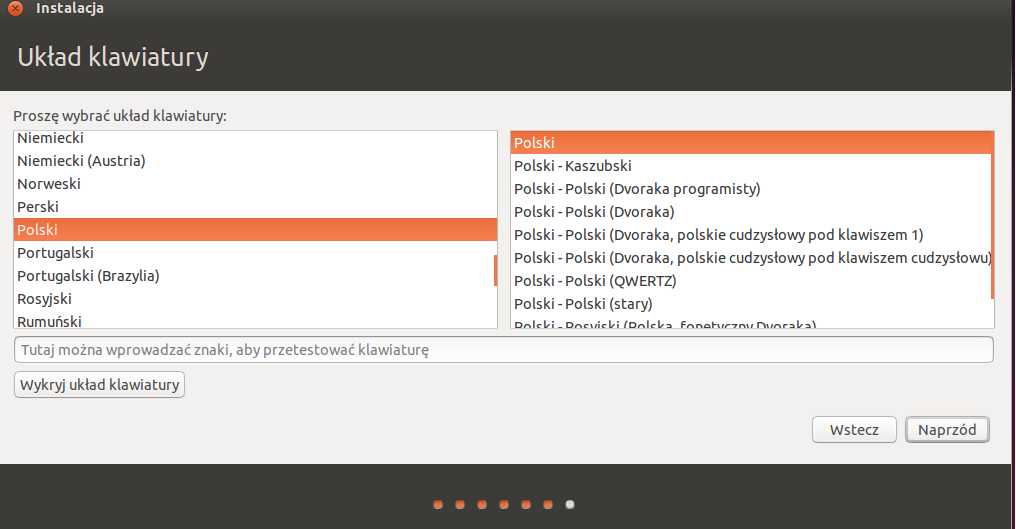
\includegraphics[width=\linewidth]{images/instalator_klawiatura.png}
\end{center}

Ten ekran pozwala wybrać układ klawiatury. Jeżeli wybrałeś wcześniej język polski, to standardowa polska klawiatura zostanie wybrana automatycznie. W polu możesz wpisać kilka znaków, aby sprawdzić, czy zaznaczony układ odpowiada rzeczywistości. Pierwsza opcja (\textcolor{ubuntu_orange}{Polski}) to standardowa klawiatura mieszcząca 101 klawiszy, zwana potocznie układem programisty.
Nie zalecamy korzystania z funkcji \textcolor{ubuntu_orange}{Wykryj układ klawiatury}. Korzystając ze wskazówek instalatora otrzymamy klawiaturę amerykańską, nieobsługującą polskich znaków diakrytycznych.
\begin{flushright}
Kliknij przycisk \textcolor{ubuntu_orange}{Naprzód}, aby przejść dalej.
\end{flushright}
\clearpage
\subsubsection{Tożsamość użytkownika}
\begin{center}
        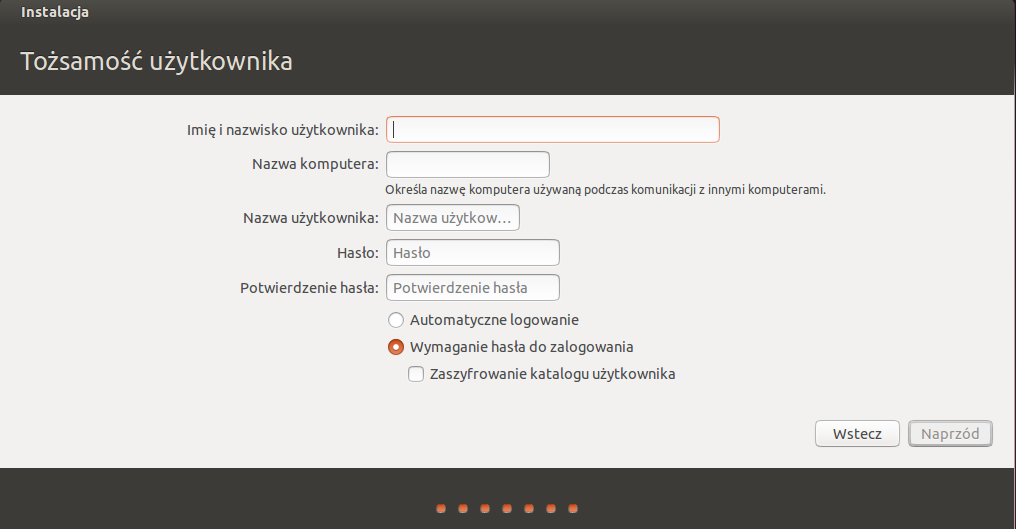
\includegraphics[width=\linewidth]{images/instalator_dane.png}
\end{center}

To już ostatni etap instalacji. Te pola należy uzupełnić, aby system mógł cię prawidłowo zidentyfikować.
\begin{itemize}
\item \textcolor{ubuntu_orange}{Imię i nazwisko użytkownika} --- Pole nieobowiązkowe, ale jeżeli uzupełnisz te dane, to system będzie się do ciebie zwracał imieniem i nazwiskiem, zamiast używać loginu (np. Jan Kowalski).
\item \textcolor{ubuntu_orange}{Nazwa komputera} --- Określa jak będzie się nazywał twój komputer (np. laptop).
\item \textcolor{ubuntu_orange}{Nazwa użytkownika} --- Twój login do systemu (np. jan\_kowalski albo twój pseudonim). Login nie może zawierać wielkich liter, spacji, ani znaków specjalnych.
\item \textcolor{ubuntu_orange}{Hasło} --- Hasło do komputera. Hasło zabezpiecza system przed nieuprawnionym dostępem.\\
Uwaga: Ustawienie hasła uniemożliwia innym zalogowanie się do twojego konta, jednak nie zabezpiecza twoich danych przed podejrzeniem przez inne osoby, o ile ich nie zaszyfrujesz. 
\item \textcolor{ubuntu_orange}{Potwierdzenie hasła} --- Wpisz ponownie to samo hasło, co w polu powyżej.
\item \textcolor{ubuntu_orange}{Automatyczne logowanie} --- Jeżeli zaznaczysz to pole, system automatycznie zaloguje tego użytkownika po uruchomieniu. Nie będzie potrzebne podawanie hasła, aby uzyskać dostęp do komputera.
\item \textcolor{ubuntu_orange}{Wymaganie hasła do zalogowania} --- Po uruchomieniu komputera będziesz musiał podać hasło, aby uzyskać dostęp do swojego konta.
\item \textcolor{ubuntu_orange}{Zaszyfrowanie katalogu użytkownika} --- Jeżeli zaznaczysz to pole, twoje prywatne dane zostaną zaszyfrowane. Nikt nieznający hasła nie będzie mógł uzyskać dostępu do twoich plików. Jeżeli zapomnisz hasło, to bezpowrotnie utracisz dostęp do swoich plików.
\end{itemize}
\begin{flushright}
Kliknij przycisk \textcolor{ubuntu_orange}{Naprzód}, aby przejść dalej.
\end{flushright}
\clearpage
\subsubsection{Instalacja}
\begin{center}
        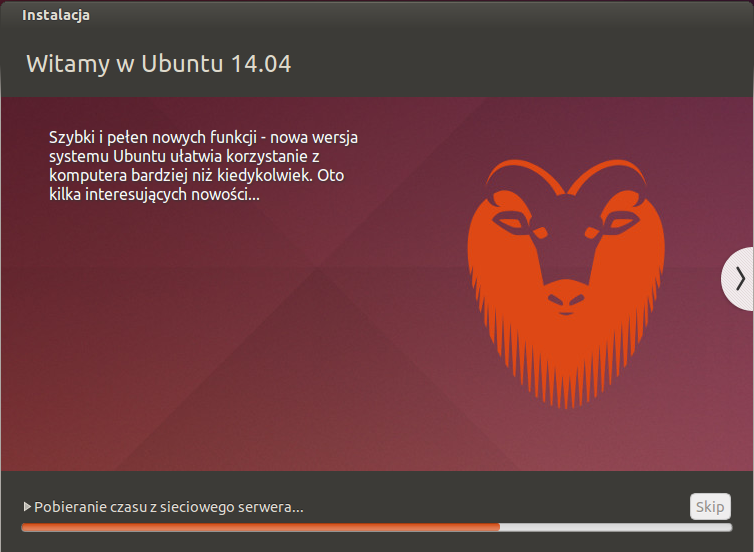
\includegraphics[width=\linewidth]{images/instalator_kopiowanie.png}
\end{center}

Teraz system dokona instalacji na dysku twardym oraz ewentualnie pobierze i zainstaluje paczki językowe, aktualizacje i dodatkowe oprogramowanie. Proces ten może potrwać od kilku, do kilkunastu minut w zależności od klasy komputera, ilości zadań do wykonania oraz szybkości łącza internetowego.
Po zakończeniu instalacji zostaniesz poproszony o usunięcie nośnika instalacyjnego i ponowne uruchomienie komputera. Jeżeli wszystko poszło pomyślnie, to za minutę zostaniesz przywitany pulpitem Ubuntu.
\begin{flushright}
\textcolor{ubuntu_orange}{Gratulacje!} Właśnie zainstalowałeś Ubuntu 14.04 LTS Trusty Tahr.\\
Komputer zostanie zresetowany.\\
Przejdź do sekcji \ref{pierwsze_uruchomienie}:,,Pierwsze Uruchomienie Ubuntu''.
\end{flushright}
\clearpage

        \subsection{Partycjonowanie dysku twardego}
                \label{subsec:partycjonowanie}
Patrycjonowanie to proces zmiany układu partycji na dysku twardym. Jest to najważniejszy etap instalacji systemu gdyż to od niego w dużej mierze zależy jak system będzie działał. Pamiętaj, że na tym etapie pracujesz na danych zapisanych na dysku twardym. Chwila nieuwagi może spowodować utratę jego zawartości.
\subsubsection{Ile miejsca przeznaczyć na Ubuntu}
\label{subsubsec:ile_miejsca}
Wirtualny dysk twardy użyty w tym przewodniku ma tylko 26.8 gigabajta pojemności. Twój dysk twardy będzie miał zapewne kilkaset gigabatów (jeżeli nie kilka terabajtów) pojemności. Dlatego też liczby jkimi się tu posługujemy będą miały niewielkie przełożenie na sytuację na twoim komputerze. W tym miejscu powinieneś się jednak zastanowić ile miejscach chcesz przeznaczyć na Ubuntu.

Ogólnie rzecz ujmując sprawa wygląda następująco
\begin{description}
\item[Partycja główna, root, /] - 6,2 Gigabajta to apsolutne minimum. 10 gigabajtów da pewną elastyczność i pozwoli zainstalować więcej programów. Nie ma potrzeby przesadzać w drugą stronę i tworzyć zbyt dużej partycji głównej, gdyż wolna przestrzeń będzie niewykorzystana. 15-20 gigabajtów w zupełności wystarczy.
\item[Partycja wymiany, swap] - na tej partycji zapisywane są dane, które nie mieszczą się w pamięci operacyjnej. Tutaj też przechowywany jest obraz RAMu kiedy poddajesz komputer hibernacji. Jeżeli korzystasz z hibernacji to wielkość partycji swap powinna być conajmniej taka jak ilość pamięci operacyjnej twojego komputera. Jeżeli nie planujesz korzystać z hibernacji to możesz nie tworzyć partycji wymiany. Jednak zaleca się jej stworzenie, jeżeli masz mniej niż 2 gigabajty RAMu. W takim wypadku nawet jeżeli nie korzystasz z hibernacji to dobrze jest stworzyć niewielką (300 - 400 megabajtów) partycję swap.
\item[Partycha domowa, /home] - W katalogu /home przechowywane są prywatne pliki użytkownika: zawartość pulpitu, dokumenty, filmy, muzyka i ustawienia programów. Katalog domowy może znajdować się na głównej partycji (/, root) lub można go wydzieć. Dobrą praktyką jest wydzielenie takiej partycji, gdyż w razie reinstalacji systemu nie trzeba będzie jej kasować. Nadpisana pozostanie tylko partycja główna, zaś wszystkie prywatne dane pozostaną niezmienione. Wielkość tej partycji zależy tylko i wyłącznie od tego jak wiele miejsca chcesz na nią przeznaczyć i jak wiele rzeczy zamierzasz na niej trzymać. 
\end{description}
\clearpage
\subsubsection{Czysty dysk - wykorzystanie całego dostępnego miejsca}
\begin{center}
	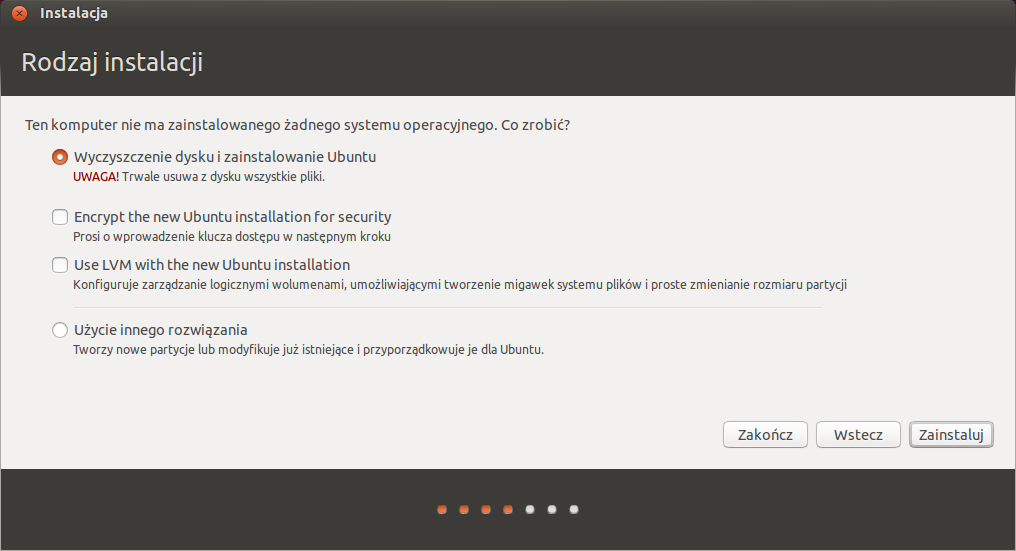
\includegraphics[scale=0.5]{images/instalator_partycjonowanie_proste.png}
\end{center}

Jeżeli na dysku twardym nie ma żadnego innego systemu operacyjnego, instalator ubuntu zaproponuje wykorzystanie całej dostępnej przestrzeni. Instalator sam dobierze odpowiedni rozmiar partycji systemowej, partycji wymiany oraz partycji użytkownika.
\begin{flushright}
Kliknij na przycisk \textbf{Zainstaluj} aby przejść dalej.\\
Zostaniesz poproszony o potwierdzenie. Upewnij się, że wszystko jest w pożądku i kliknij \textbf{Naprzód}.\\
W tym momencie wybrane zmiany zostaną zapisane na dysku twardym.
\end{flushright}
\clearpage

\subsubsection{Instalacja obok zainstalowanego Ubuntu}
\begin{center}
	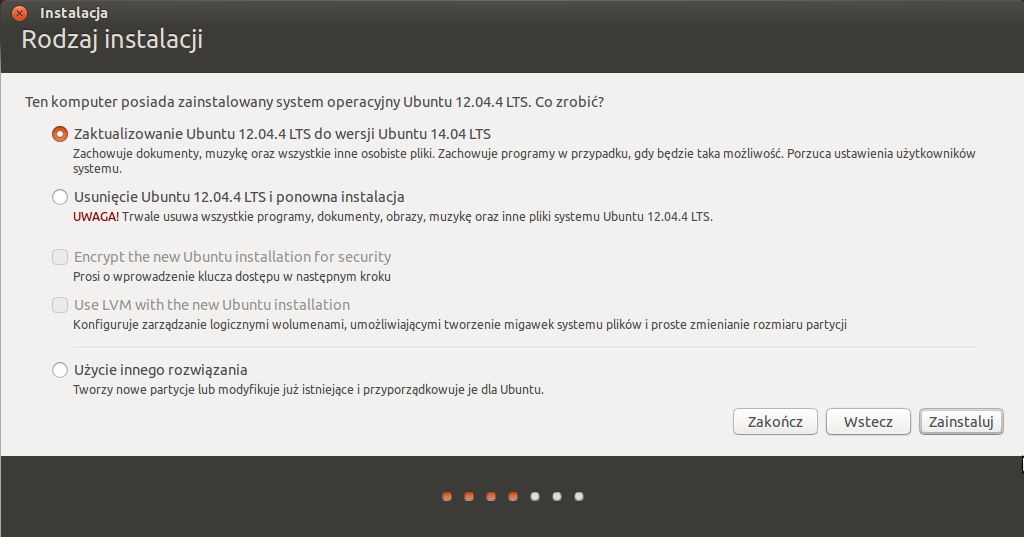
\includegraphics[scale=0.5]{images/instalator_partycjonowanie_obok_ubuntu.png}
\end{center}
Jeżeli instalator wykryje obecność wcześniej zainstalowanej innej wersji Ubuntu to zaproponuje kilka innych rozwiązań.

Po pierwsze zaproponuje aktualizację zainstalowanego systemu do najnowszego wydania. Wszystkie dane w katalogu domowym użytkownika zostaną zachowane: muzyka, filmy, dokumenty, pliki na pulpicie, osobieste ustaienia programów, zakładki i historia przeglądarki itp.
Skasowane zostaną zainstalowane w systemie programy oraz ustawienia systemowe. Instalator zaktualizuje istniejące na dysku oprogramowanie i ewentualnie pobierze aktualizacje z internetu (jeżeli wybrałeś wcześniej tą opcję).

Drugą opcją jest usunięcie zainstalowanego Ubuntu i ponowna instalacja systemu. Wszystkie dane zostaną wymazane.
\begin{flushright}
Kliknij na przycisk \textbf{Zainstaluj} aby przejść dalej.\\
Zostaniesz poproszony o potwierdzenie. Upewnij się, że wszystko jest w pożądku i kliknij \textbf{Naprzód}.\\
W tym momencie wybrane zmiany zostaną zapisane na dysku twardym.
\end{flushright}
\clearpage

\subsubsection{Instalacja obok Windowsa}
\begin{center}
	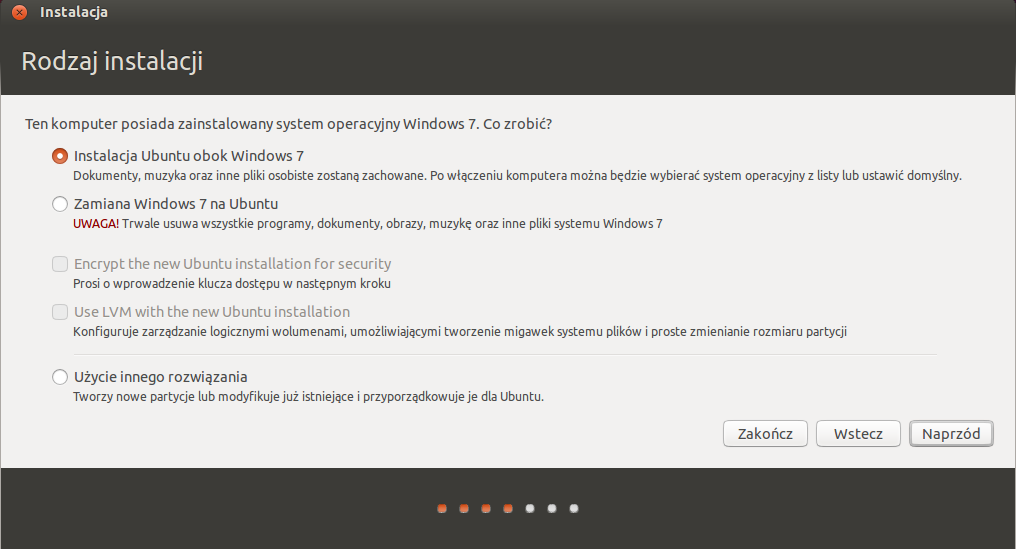
\includegraphics[scale=0.5]{images/instalator_partycjonowanie_obok_wondows7.png}
\end{center}
Jeżeli instalator wykryje obecnosć wcześniej zainstalowanego systemu Windows to zaproponuje inne rozwiązanie. Opcja "Zamiana Windows na Ubuntu" wymaże całą zawartość partycji Windows (wraz ze wszystkimi danymi) i zamiast tego zainstaluje Ubuntu. Zostało to opisane dwie strony wcześniej.
\begin{flushright}
Kliknij na przycisk \textbf{Zainstaluj} aby przejść dalej.
\end{flushright}
\clearpage
\begin{center}
	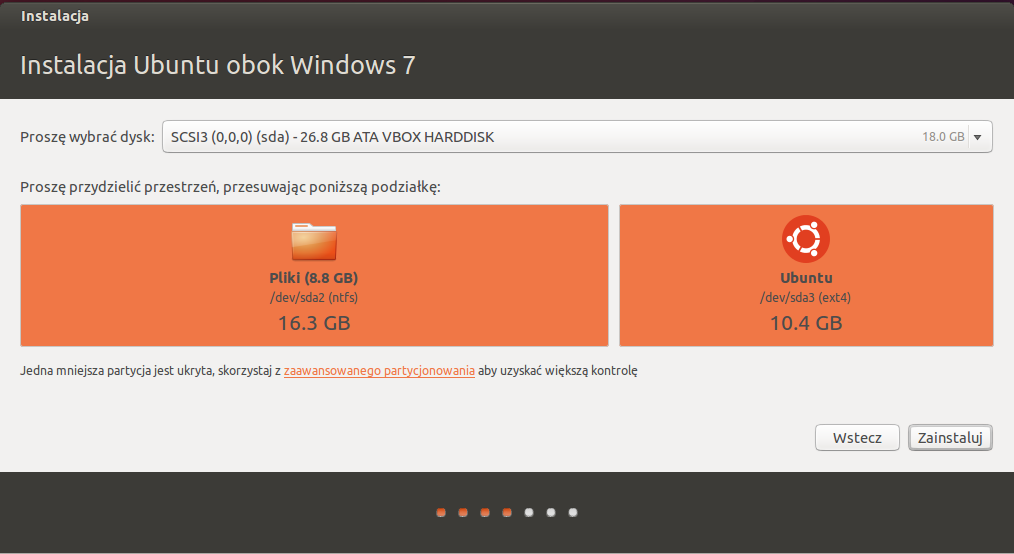
\includegraphics[scale=0.5]{images/instalator_partycjonowanie_obok_wondows7_2.png}
\end{center}
Drugą możliwością jest instalacja Ubuntu obok już zainstalowanego systemu Windows. Jeżeli wybierzesz tę opcję to następny ekran pozwoli wybrać o ile instalator ma zmniejszyć partycję na której zainstalowany jest system Windows. Użyj myszy aby przesunąć pomarańczową podziałkę w lewo (więcej miejsca dla Ubuntu) lub w prawo(więcej miejsca dla Windowsa). Oryginalna partycja systemu Windows jest oznaczona na tym obrazie jako "Pliki". Pamiętaj, że ubuntu potrzebuje minimum 6,2 gigabajta przestrzeni, ale tak mała partycja zostanie prawie w całości wypełniona przez system i na Twoje pliki pozostanie niewiele miejsca.

\begin{flushright}
Kliknij na przycisk \textbf{Zainstaluj} aby przejść dalej.\\
Zostaniesz poproszony o potwierdzenie. Upewnij się, że wszystko jest w pożądku i kliknij \textbf{Naprzód}.\\
W tym momencie wybrane zmiany zostaną zapisane na dysku twardym.
\end{flushright}
\clearpage

\subsubsection{Szyfrowanie dysku twardego}
\begin{center}
	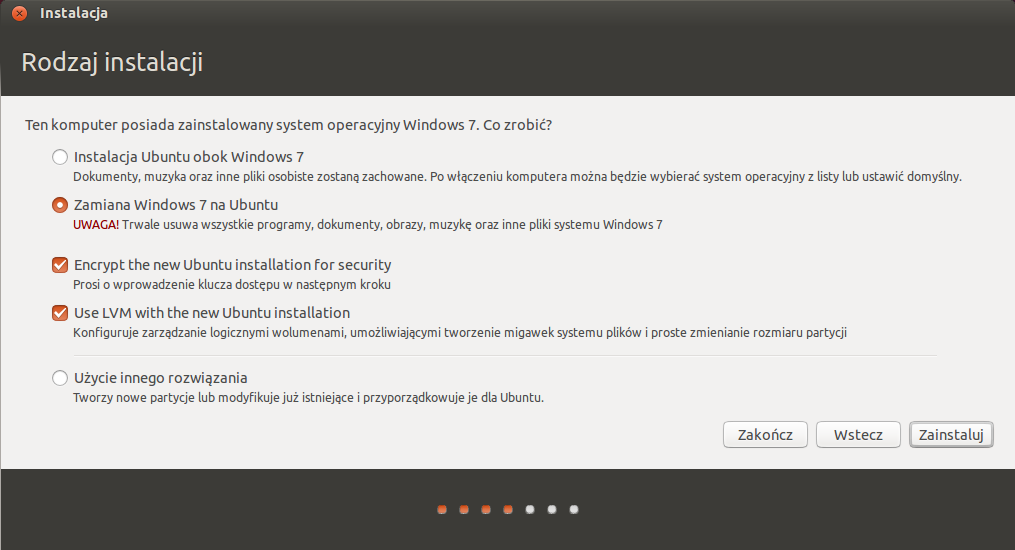
\includegraphics[scale=0.5]{images/instalator_partycjonowanie_szyfrowanie1.png}
\end{center}
Przy wyborze jednego z automatycznych rozwiązań partycjonowania miałeś możliwości zastosowania szyfrowania dysku twardego. Wybranie tej opcji ukaże ci okno jak na powyższym obrazku. Zaszyfrowanie dysku twardego sprawie, że nikt nie uzyska dostępu do twoich danych ani nie zmodyfikuje zainstalowanego systemu. Wadą tego rozwiązania jest pewien narzut na procesor komputera i związane z tym zmniejszenie płynności działania komputera. Nowoczesne procesory zapewniają akcelerację sprzętową dla obliczeń kryptograficznych, w związku z czym utrata wydajności będzie się mieścić w granicach 5\% przy intensywnych opracacjach dyskowych.
\begin{flushright}
Kliknij na przycisk \textbf{Zainstaluj} aby przejść dalej.
\end{flushright}
\clearpage
\begin{center}
	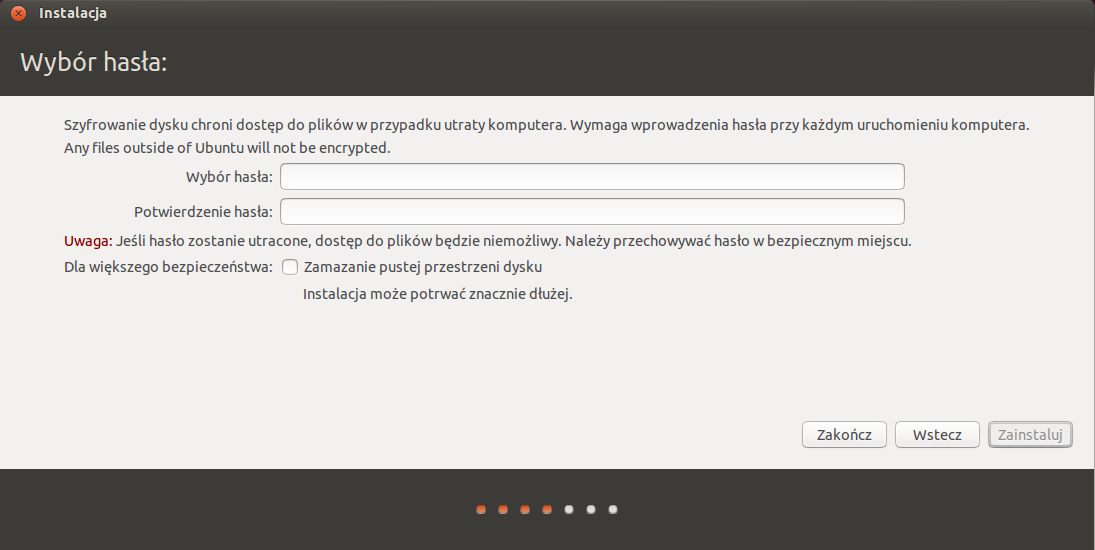
\includegraphics[scale=0.5]{images/instalator_partycjonowanie_szyfrowanie2.png}
\end{center}
Na tym ekranie podaj hasło - klucz do dysku twardego. To nie jest to samo hasło, które ustawisz dla swojego systemowego konta a jedynie hasło umożliwiające dostęp do danych zapisanych na dysku twardym. Pamiętaj, że jeżeli zapomnisz hasła jakie zostanie tu wprowadzone, nie będzie możliwości odzyskania zaszyfrowanych danych. Postaraj się też aby hasło nie było łatwe do odgadnięcia, ale łatwe dla ciebie do zapamiętania.

Opcja "Zamazanie pustej przestrzeni dysku" powoduje, że niewykorzystywana, wolna przestrzeń dysku zostanie nadpisana losowymi danymi. Taka operacja znacznie utródnia potencjalnym włamywaczą włamanie się do twoich danych. Miej na uwadze, że zamazywanie pustej przestrzeni może trwać bardzo długo, w zależności do tego ile miejsca przeznaczysz na Ubuntu.

\begin{flushright}
Kliknij na przycisk \textbf{Zainstaluj} aby przejść dalej.\\
Zostaniesz poproszony o potwierdzenie. Upewnij się, że wszystko jest w pożądku i kliknij \textbf{Naprzód}
W tym momencie wybrane zmiany zostaną zapisane na dysku twardym.\\
\end{flushright}
\clearpage

\subsection{Zaawansowane partycjonowanie}
\begin{center}
	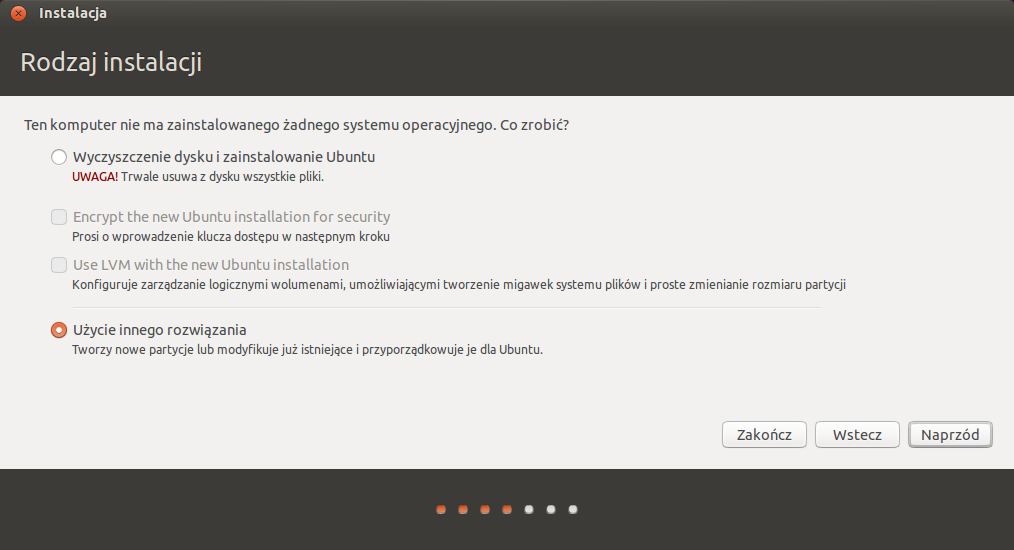
\includegraphics[scale=0.5]{images/instalator_partycjonowanie_gparted1.png}
\end{center}
"Użycie innego rozwiązania" uruchamia program GParted, który umożliwia nieograniczone modyfikowanie partycji na dysku twardym. Jest to opcja dla bardziej zaawansowanych użytkowników, którzy mają świadomość tego jak działa partycjonowanie i jak powinien zostac podzielony ich dysk twardy. Jednak jeżeli na swoim komputerze maasz zainstalowany więcej niż jeden system operacyjny lub z jakiegoś innego powodu przedstawione wcześniej opcje nie spełniają twoich wymagań, to konieczne będzie sięgnięcie do zaawansowanego partycjonowania.

Do GParted warto zajrzeć jeszcze z jednego powodu. Podział partycji stosowany przez automatyczną instalację nie jest idealny. Ręczne ustawienie partycji da większa kontrolę i pozwoli znacznie lepiej dopasować układ partycji.
\begin{flushright}
Kliknij na przycisk \textbf{Naprzód} aby przejść dalej.
\end{flushright}
\clearpage

\subsubsection{Główne okno programu GParted}
\begin{center}
	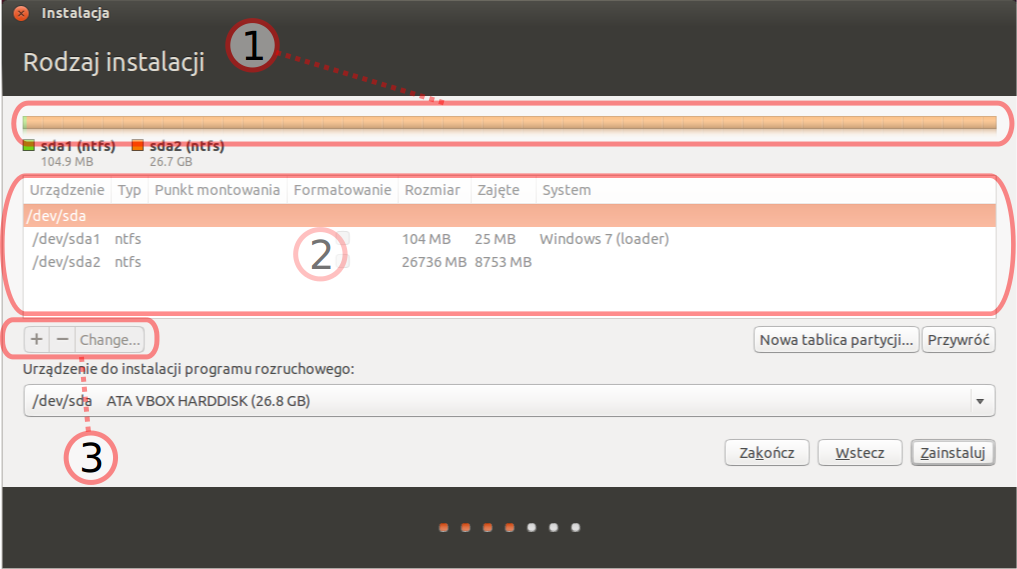
\includegraphics[scale=0.5]{images/instalator_partycjonowanie_gparted2.png}
\end{center}
Na powyższym obrazku widzisz głowne okno programu GParted. Wykryty został układ partycji na dysku twardym. Poziomy pasek (1) rozciągający się na całą szerokość okna jest graficzną reprezentacją układu partycji. Poniżej paska znajduje się legenda objaśnijaca użyte kolory. Tabela (2) znajdująca się w centralnej części okna przedstawia szczegółowe informacje na temat partycji na dysku twardym. Zestaw przycisków (3) służy do dodawania partycji(+), usówania partycji (-) lub ich modyfikacji(Change). Na chwilę obecną inne rzeczy nas nie interesują.

Powyższy układ dysków twardych oraz partycji jest tylko przykładem skonstruowanym na maszynie wirtualnej. Na Twoim komputerze liczby będą inne.

\clearpage
\begin{center}
	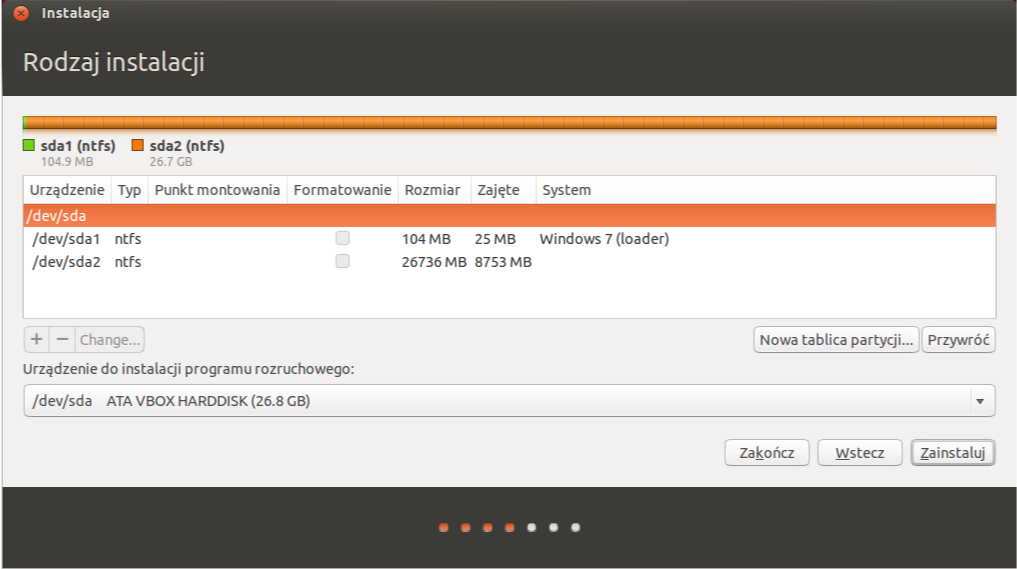
\includegraphics[scale=0.5]{images/instalator_partycjonowanie_gparted2_czysty.png}
\end{center}
Tabela umieszczona w centrum tego okna przedstawia informacje o poszczególnych partycjach obecnych na dysku twardym. Objaśnienie poszczególnych kolumn:
\begin{description}
\item[Urzadzenie] - Ścierzka do poszczególnych partycji na dysku twardym. Są to oznaczenia stosowane w systemach Unikoswych, do których należy Linux a więc i Ubuntu i opisują jak rozpoznawane są poszczególne partycje. W tym wypadku:
	\begin{description}
	\item[/dev/] - skrót od "Device", urządzenie
	\item[sda] - oznaczenie pierwszego dysktu twardego.
		\begin{description}
			\item[sd] - dysk na złączu SATA (sata disc)
			\item[a] - pierwszy dysk. Drugi dysk twardy miałby literę "b", trzeci "c" i tak dalej.
		\end{description}
	\item[sda1] - pierwsza partycja na pierwszym dysku twardym.
	\item[sda2] - druga partycja na pierwszym dysku twardym.
	\end{description}
\item[Typ] - rodzaj systemu plików. Sposób w jaki partycja została sformatowana. System Windows korzysta z ntfs, Ubuntu może korzystać z różnych.
\item[Punkt montowania] - miejsce w którym dana partycja zostanie "zamontowana", katalog w którym będzie widoczna zawartość tej partycji.
\item[Formatowanie] - zaznaczając to pole informujesz instalator, że dana partycja ma zostać sformatowana. Oznacza to utratę wszystkich danych na niej zapisanych.
\item[rozmiar] - pojemność partycji w megabajtach.
\item[Zajęte] - ile miejsca zostało zajęte na tej partycji
\item[System] - system operacyjny zainstalowany na danej partycji. Nie zawsze da się rozpoznać zainstalowany system. Nie każda partycja musi mieć zainstalowany system operacyjny. 
\end{description}
\clearpage
\subsubsection{Zaawansowane partycjonowanie - Instalacja obok systemu Windows}
\begin{center}
	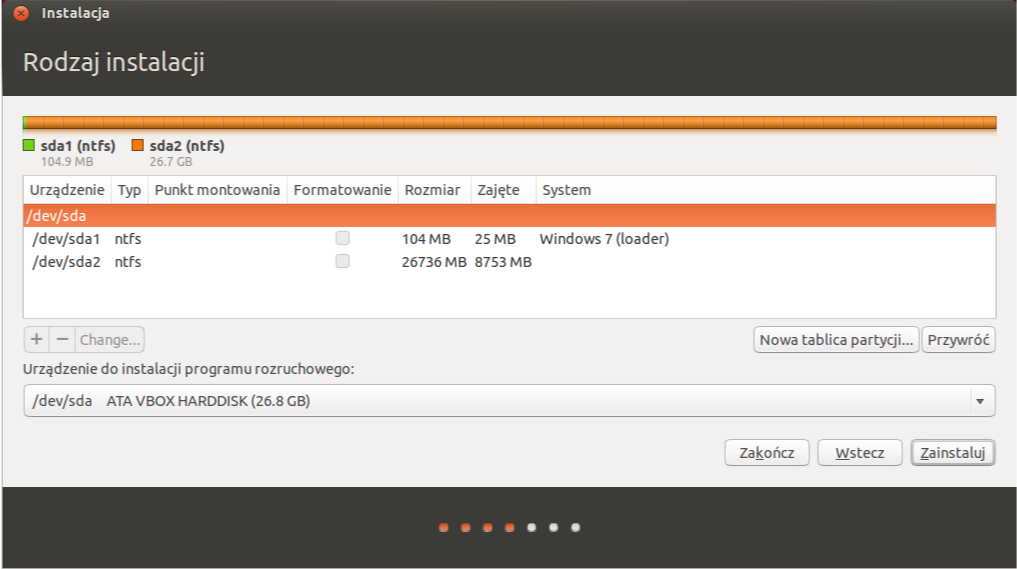
\includegraphics[scale=0.5]{images/instalator_partycjonowanie_gparted2_czysty.png}
\end{center}

Na powyższym obrazku widać dwie partycje utworzone przez instalator systemu Windows7. Partycja zielona o rozmiarze 104 megabajtów służy jako partycja dla programu rozruchowego systemu Windows. Duża, pomarańczowa partycja (26736 megabajtów) jest główna partycją systemu Windows7. Bardzo podobny układ partycji stosowany jest przez każdy z systemów z rodziny Windows.

Pierwszym krokiem jest zrobienie miejsca dla systemu Ubuntu. Kliknij na partycję /dev/sda2. Następnie kliknij na przycisk "Change" znajdujący się pod tabelą.. W otwartym oknie możesz zmniejszyć rozmiar wybranej partycji.
\clearpage

\begin{wrapfigure}{R}{0.4\textwidth}
		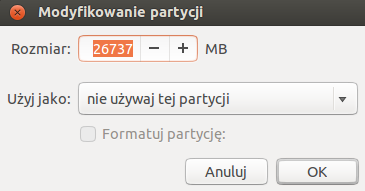
\includegraphics[scale=1]{images/instalator_partycjonowanie_gparted_zmniejszenie_partycji_windows.png}
\end{wrapfigure}
W polu Rozmiar podaj nowy rozmiar partycji. O tym ile miejsca potrzebujesz na Ubuntu przeczytasz w rozdziale \ref{subsubsec:ile_miejsca}: Ile miejsca przeznaczyć na Ubuntu. W polu podajesz rozmiar partycji w megabajtach. Jeden gigabajt to 1024 megabajty.\\
Upewnij się, że wybrano opcję "nie używaj tej partycji". Teraz kliknij przycisk \textbf{OK} a następnie \textbf{Naprzód} aby dokonać zmiany na partycji. Wykonanie żądanej zmiany może trwać dłuższą chwilę.

Na schemacie pojawiła się pusta, "dostępna przestrzeń" oznaczona kolorem szarym. Kliknij a nią, a następnie na przycisk (+) aby stworzyć nową partycję.
\begin{center}
	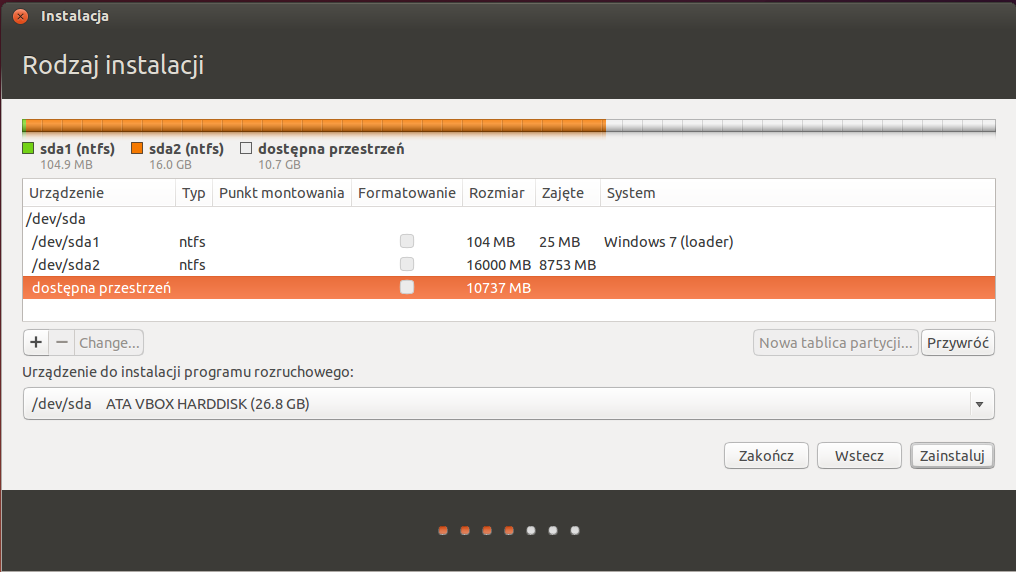
\includegraphics[scale=0.7]{images/instalator_partycjonowanie_gparted3.png}
\end{center}
\clearpage

\begin{wrapfigure}{R}{0.4\textwidth}
		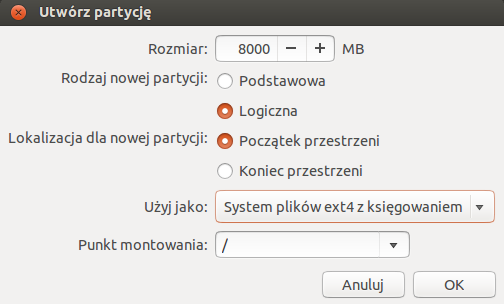
\includegraphics[scale=0.8]{images/instalator_partycjonowanie_gparted_dodaj_root.png}
\end{wrapfigure}
Po pierwsze musimy stworzyć partycję podstawową dla Ubuntu. O ilości miejsca potrzebnej na poszczególne partycje przeczytasz w sekcji \ref{subsubsec:ile_miejsca}: "Ile miejsca przeznaczyć na Ubuntu". Pozostałe opcje ustaw jak na rysunku.
\begin{description}
\item[Rozmiar] - rozmiar partycji w megabajtach
\item[Rodzaj nowej partycji] - jako, że system Windows korzysta z tablicy partycji ms-dos to jesteśmy ograniczeni do 4 partycji podstawowych. Aby nie było problemu, dla Ubuntu utworzymy partycje logiczne.
\item[Lokalizacja dla nowej partycji] - Czy partycja zostanie wyrównana do poczatku wolnej przestrzeni czy do jej końca. Nie ma to znaczenia dla działania systemu.
\item[Użyj jako] - jaki system plików ma być użyty do sformatowania tej partycji. Do wyboru jest wiele, ale w ramach tego przewodnika korzystamy z systemu ext4 z księgowaniem\footnote{Tematyka różnych systemów plików jest bardzo rozległa i z łatwością wypełniłaby kolejny Przewodnik.}
\item[Punkt montowania] - to nasza główna partycja, więc musi się znaleźdź na początku\footnote{W systemach Windows drzewo katalogów "zaczyna się" na "C:\textbackslash\textbackslash". W systemach Linuksowych zaczyna się na "/"}.
\end{description}
Kliknij na przycisk \textbf{OK} aby utworzyć nową partycję.
\clearpage
\begin{wrapfigure}{R}{0.4\textwidth}
		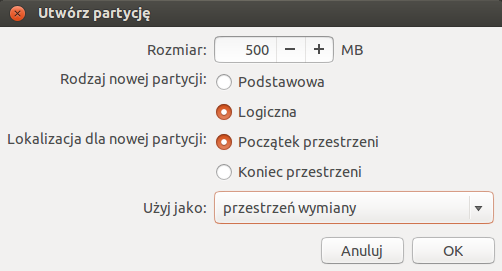
\includegraphics[scale=0.8]{images/instalator_partycjonowanie_gparted_dodaj_swap.png}
\end{wrapfigure}
Teraz utwórz partycję wymiany. Więcej o tej partycji przeczytasz w w sekcji \ref{subsubsec:ile_miejsca}: "Ile miejsca przeznaczyć na Ubuntu". Pozostałe opcje ustaw jak na rysunku. Kliknij na przycisk \textbf{OK} aby utworzyć nową partycję.

\begin{wrapfigure}{L}{0.4\textwidth}
		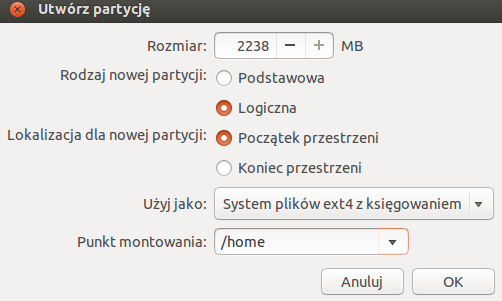
\includegraphics[scale=0.8]{images/instalator_partycjonowanie_gparted_dodaj_home.png}
\end{wrapfigure}
Na koniec pozostało utworzenie partycji domowej. Więcej o tej partycji przeczytasz w w sekcji \ref{subsubsec:ile_miejsca}: "Ile miejsca przeznaczyć na Ubuntu". Pozostałe opcje ustaw jak na rysunku. Kliknij na przycisk \textbf{OK} aby utworzyć nową partycję.
\clearpage

\begin{center}
	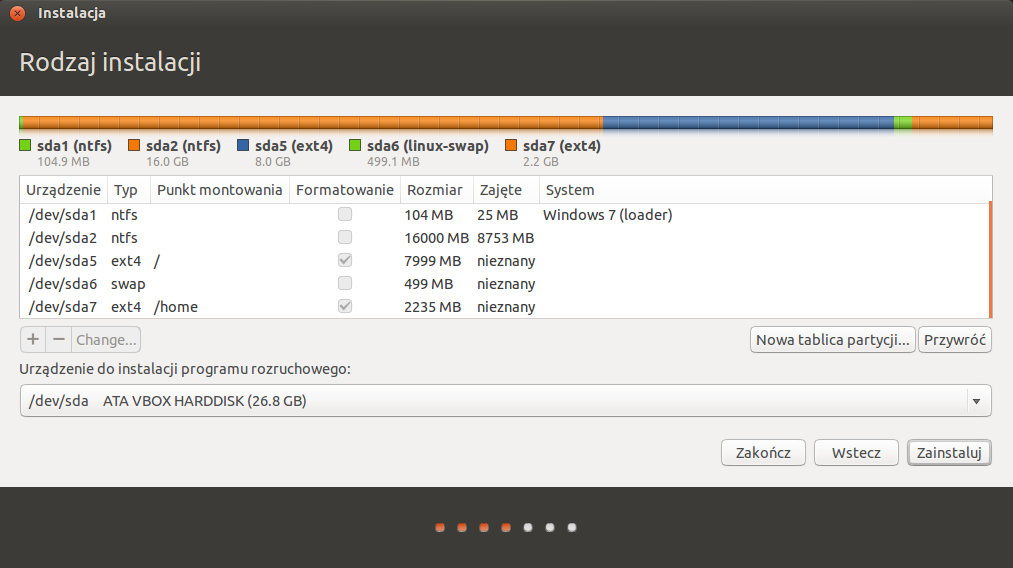
\includegraphics[scale=0.7]{images/instalator_partycjonowanie_gparted4.png}
\end{center}
Ekran programu GParted wygląda teraz mniej więcej tak jak na rysunku powyżej. Masz dwie partycje systemu Windows (ntfs), partycję wymiany systemu Linux (swap) oraz dwie partycje dla systemu Ubuntu (ext4). Upewnij się, że partycje ntfs \textbf{nie} są zaznaczone do sformatowania, zaś partycje ext4 tak. Kliknij na przycisk \textbf{Naprzód} aby wprowadzić zmiany na partycjach. Teraz możesz powrócić do lektury procesu instalacji w miejscu gdzie go przerwałeś.\\
Powrót do \ref{subsub:instalator_strefa_czasowa}: Wybór sterfy czasowej.
\clearpage
        \subsection{Instalacja na maszynie wirtualnej}
                \begin{wrapfigure}{L}{0.5\textwidth}
	\vspace{-10pt}
	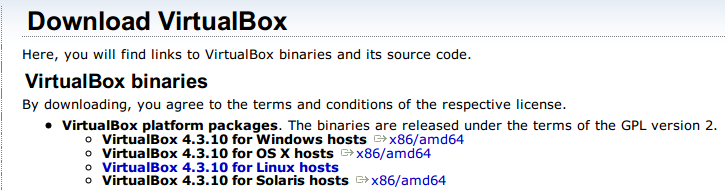
\includegraphics[width=\linewidth]{images/virtualbox_download.png}
\end{wrapfigure}

Alternatywnym sposobem wypróbowania Ubuntu bez instalowania go bezpośrednio na komputerze jest wykorzystanie maszyny wirtualnej. Specjalne oprogramowanie umożliwia uruchomienie systemu operacyjnego, zwanego ,,gościem'', jako programu działającego wewnątrz drugiego systemu, zwanego ,,gospodarzem''. Wiąże się to oczywiście z dużym zapotrzebowaniem na moc obliczeniową procesora oraz pamięć operacyjną. Jeżeli masz przynajmniej 2 gigabajty RAM-u, a twój procesor jest nie starszy niż 5 lat (wtedy jest szansa, że będzie zapewniał akcelerację sprzętową dla wirtualizacji), to możesz w ten sposób wypróbować Ubuntu.

\begin{wrapfigure}[11]{r}{0.5\textwidth}
	\vspace{-10pt}
	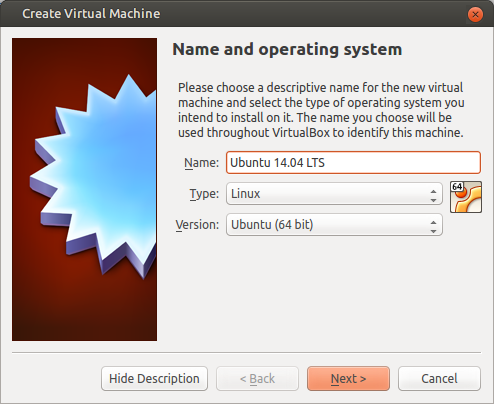
\includegraphics[width=\linewidth]{images/virtualbox_wizard1.png}
\end{wrapfigure}

Jedną z najpopularniejszych maszyn wirtualnych jest VirtualBox. Otwórz stronę \href{https://www.virtualbox.org/wiki/Downloads}{virtualbox.org/download} i pobierz instalator VirtualBoksa dla swojego systemu. Zainstaluj, a następnie uruchom program VirtualBox. Podczas pierwszego uruchomienia program zapyta cię, czy pobrać i zainstalować dodatkowe rozszerzenia od Oracle. Zgódź się na to.

W oknie głównym programu VirtualBox kliknij przycisk \textcolor{ubuntu_orange}{New}, aby uruchomić kreator maszyny wirtualnej.

\begin{itemize}
\item \textcolor{ubuntu_orange}{Name} --- nazwa maszyny wirtualnej. Może to być cokolwiek.
\item \textcolor{ubuntu_orange}{Type} --- typ systemu. Ustaw na \textcolor{ubuntu_orange}{Linux}.
\item \textcolor{ubuntu_orange}{Version} --- wersja systemu. Ustaw na \textcolor{ubuntu_orange}{Ubuntu (64 bit)}.\\
Uwaga: Architektura wybranego systemu (32/64 bit) musi odpowiadać pobranemu obrazowi instalatora Ubuntu. Dodatkowo należy pamiętać, że w komputerze z 64-bitowym procesorem (najprawdopodobniej taki posiadasz, jeżeli twój komputer nie jest starszy niż 6 lat) można zainstalować zarówno 64-, jak i 32-bitowy system-gościa, natomiast w komputerze z procesorem 32-bitowym --- jedynie 32-bitowy.
\end{itemize}
\begin{flushright}
Kliknij przycisk \textcolor{ubuntu_orange}{Next}, aby przejść dalej.
\end{flushright}

\clearpage
\begin{wrapfigure}{r}{0.5\textwidth}
	\vspace{-10pt}
	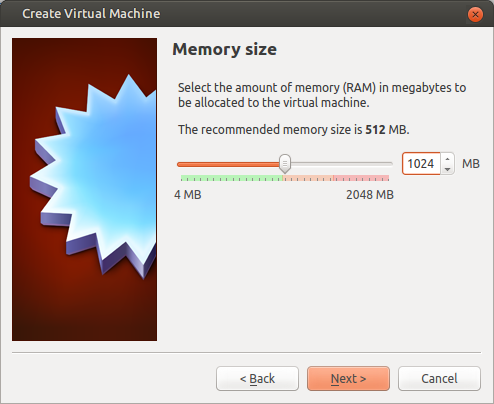
\includegraphics[width=\linewidth]{images/virtualbox_wizard2.png}
\end{wrapfigure}

W tym miejscu ustaw ilość pamięci operacyjnej twojego komputera, jaką chcesz przeznaczyć dla systemu-gościa. Weź pod uwagę, że ta pamięć zostanie zajęta w momencie uruchomienia maszyny wirtualnej i nie będzie dostępna dla systemu-gospodarza. Nie powinno się przydzielać gościowi więcej niż 50\% zasobów gospodarza. Ubuntu wymaga minimum 512 megabajtów (system plus oprogramowanie), a zdecydowanie lepiej jest przydzielić 1024 megabajty. Jeżeli twój komputer posiada tylko 2 gigabajty RAM-u, to przydzielając 1~gigabajt gościowi pozostanie tylko 1 gigabajt dla gospodarza. Nie jest to dobre rozwiązanie, gdyż prawdopodobnie będziesz musiał wyłączyć większość programów w systemie-gospodarzu, aby nie doszło do przepełnienia pamięci operacyjnej. Na pewno będziesz musiał wyłączyć przeglądarkę internetową.

\begin{flushright}
Kliknij przycisk \textcolor{ubuntu_orange}{Next}, aby przejść dalej.
\end{flushright}

W kolejnym oknie można wybrać już istniejący wirtualny dysk twardy lub stworzyć nowy. Ponieważ nie masz jeszcze żadnego takiego urządzenia, wybierz środkową opcję \textcolor{ubuntu_orange}{Create a virtual hard drive now}.
\begin{flushright}
Kliknij przycisk \textcolor{ubuntu_orange}{Next}, aby przejść dalej.
\end{flushright}

W kolejnym oknie wybierz typ dysku twardego. Zaznacz opcję \textcolor{ubuntu_orange}{VDI (Virtual Disk Image)}.
\begin{flushright}
Kliknij przycisk \textcolor{ubuntu_orange}{Next}, aby przejść dalej.
\end{flushright}

W kolejnym oknie wybierz pomiędzy dyskiem tworzonym dynamicznie, a dyskiem o stałym rozmiarze.
\begin{itemize}
\item \textcolor{ubuntu_orange}{Dynamically allocated} --- taki wirtualny dysk twardy nie zajmuje całego przydzielonego miejsca, a jedynie tyle, ile wynosi suma rozmiaru plików na nim zapisanych. Nawet jeżeli stworzysz dysk o pojemności 100 gigabajtów, to po instalacji Ubuntu będzie on zajmował tylko trochę ponad 6 gigabajtów w systemie-gospodarzu. Wybierz tę opcję.
\item \textcolor{ubuntu_orange}{Fixed size} --- taki dysk twardy zawsze zajmuje tyle miejsca w systemie-gospodarzu, ile zostało zadeklarowane. Jeżeli stworzysz 100-gigabajtowy dysk wirtualny, to na twoim komputerze pojawi się 100-gigabajtowy plik z maszyną wirtualną. Tworzenie takiego dysku też trwa dłuższą chwilę, gdyż dużo danych musi zostać zapisanych na dysk.
\end{itemize}
\begin{flushright}
Kliknij przycisk \textcolor{ubuntu_orange}{Next}, aby przejść dalej.
\end{flushright}
\clearpage
\begin{wrapfigure}[12]{r}{0.5\textwidth}
	\vspace{-10pt}
	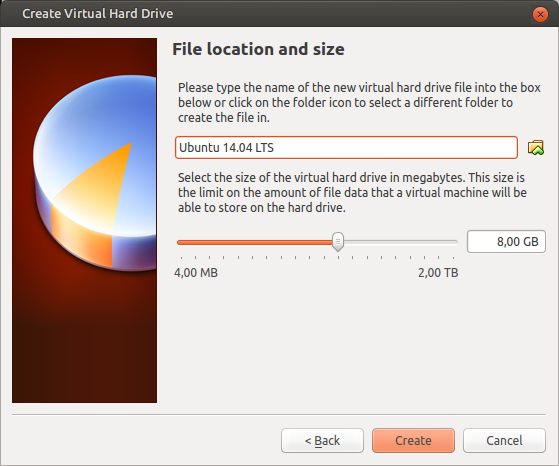
\includegraphics[width=\linewidth]{images/virtualbox_wizard6.png}
\end{wrapfigure}

Tu możesz wybrać pojemność dysku twardego. Korzystając z suwaka ustaw żądany rozmiar. Ubuntu 14.04 LTS wymaga przynajmniej 6,2 gigabajta, górną granicą są tylko możliwości VirtualBoksa (2 terabajty). W celach testowych stwórz dysk o rozmiarze przynajmniej 25 gigabajtów.

Kliknij przycisk \textcolor{ubuntu_orange}{Create}, aby stworzyć dysk i zakończyć działanie kreatora.

Twoja maszyna wirtualna dla Ubuntu jest gotowa i można ją wybrać w głównym oknie programu VirtualBox. Kliknij na jej nazwie i z paska narzędziowego wybierz \textcolor{ubuntu_orange}{Start}. Alternatywnym sposobem uruchomienia maszyny wirtualnej jest dwukrotne kliknięcie na jej ikonie. Zobaczysz okno, jak na rysunku powyżej. Kliknij żółtą ikonę folderu i wskaż pobrany wcześniej obraz instalatora systemu Ubuntu (plik .iso). Kliknij \textcolor{ubuntu_orange}{Start}, aby uruchomić maszynę wirtualną. Instalacja na maszynie wirtualnej przebiega tak samo, jak w rzeczywistości. Przejdź do sekcji \ref{instalacja_uruchomienie}: ,,Uruchomienie instalatora BIOS''.

\begin{center}
	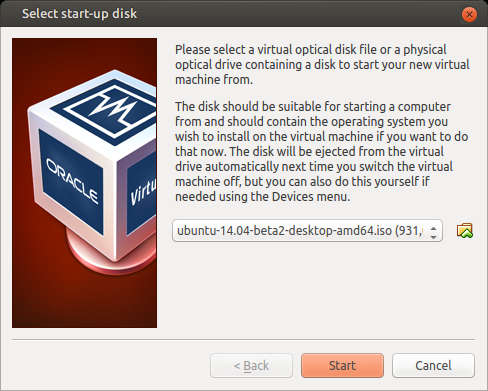
\includegraphics[width=\linewidth]{images/virtualbox_start.png}
\end{center}

Kiedy po zakończeniu instalacji zostaniesz poproszony o wyjęcie płyty instalatora z napędu, z paska menu maszyny wirtualnej wybierz \menu{{Devices}>{Cd/DVD Devices}>{Remove disk from virtual drive}}.

Żeby móc się cieszyć pełnosprawną maszyną wirtualną, należy doinstalować w systemie-gościu \textcolor{ubuntu_orange}{Używanie x86 virtualization solution --- guest addition module source for dkms z virtualbox-guest-dkms (własnościowy)}, zgodnie z instrukcją zawartą w \ref{pierwsze_uruchomienie_aktualizacja_instalacja}: ,,Instalacja dodatkowych sterowników''.
  
        \subsection{Rozwiązywanie problemów z instalacją}
                \subsubsection{Po wybraniu opcji ,,Wypróbuj Ubuntu bez instalacji'' lub ,,Instaluj Ubuntu'' mam tylko czarny ekran}
Po pierwsze odczekaj dłuższą chwilę, wczytanie wszystkich danych z nośnika instalacyjnego trwa dłuższą chwilę. Jeżeli trwa to dłużej niż 2--3 minuty to zrestartuj komputer i uruchom instalator Ubuntu jeszcze raz. W przypadku instalatora BIOS (filoetowe tło) po wybraniu języka wcśnij \keys{F6} (inne opcje), zaznacz opcję ,,nomodeset'' klawiszem \keys{\returnwin}, wyjdź z menu klawiszem \keys{Esc} i uruchom instalator. Opcja ,,acpi=off'' też może być pomocna.

\subsubsection{Instalacja została przerwana}
Jeżeli instalacja została przerwana w trakcie kopiowania danych na dysk to uruchom ponownie instalator i zainstaluj system od nowa.

Jeżeli instalacja została przerwana w trakcie partycjonowania (zapisywania zmian na dysku) to prawdopodobnie doszło do nieodwracalnego uszkodzenia tablicy partycji. Uruchom nośnik instalacyjny, wybierz ,,Wypróbuj Ubuntu bez instalacji'' (\textit{Try Ubuntu without installing''} i uruchom program GParted.

\subsubsection{Po instalacji Ubuntu uruchamia się tylko Windows}
Prawdopodobnie na Windowsie masz ustawione ,,Szybkie uruchamianie'' (\textit{Fast-boot}). Wyłącz tą funkcję i ponownie zainstaluj Ubuntu. Przeczytaj rozdział \ref{sec:przygotowanie_windows}: ,,Przygotowanie do instalacji''.

\subsubsection{Po instalacji Ubuntu nie można uruchomić systemu Windows}
przyczyny mogą być dwie. Albo usunąłeś system Windows z dysku twardego, albo nie został on prawidłowo rozpoznany. W pierwszym przypadku pozostaje tylko go ponownie zainstalować. Koniecznie przeczytaj rozdział Przeczytaj rozdział \ref{sec:przygotowanie_windows}: ,,Przygotowanie do instalacji''.

W drugim przypadku przejdź do sekcji ,,Przywracanie GRUB-a''

\subsubsection{Przywracanie GRUB-a}
\label{grub_przywracanie}
Problemy z programem rozruchowym występują najczęściej:
\begin{itemize}
\item Po instalacji systemu Windows obok Ubuntu. Windows nadpisuje MBR (\textit{Master Boot Record)} dysku twardego i uniemożliwia dostęp do systemów Linuksowych.
\item Po instalacji Ubuntu obok Windowsa, jeżeli ten był za-hibernowany, miał włączoną opcję ,,Fast-Boot'' lub podobne.
\item Po zmianie rozkładu partycji.
\item Po nieumiejętnych próbach edytowania GRUBa lub zastąpienia go innym menadżerem rozruchowym.
\end{itemize}

Najprostszym sposobem naprawienia menadżera rozruchu GRUB jest skorzystanie z boot-repair disk. Jest to dystrybucja Linuksa typu Live (działa tylko z zewnętrznego nośnika, nie zainstalujesz jej na dysku twardym). Wejdź na stronę \href{http://sourceforge.net/projects/boot-repair-cd/files/}{pobierania}, wybierz plik z obrazem zgodny z architekturą twojego procesora i zapisz go na dysku. Proces przygotowywania nośnika z Boot-Rapair disk jest analogiczny do tego przedstawionego w rozdziale \ref{nagrywanie_obrazu}: ,,Nagrywanie pobranego obrazu''.\\
Po uruchomieniu tak przygotowanego systemu poczekaj aż się załaduje i wybierz opcję \textcolor{ubuntu_orange}{Recomended repair} a nastepnie spróbuj ponownie uruchomić komputer.

Jeżeli nie możesz uruchomić żadnego systemu operacyjnego to program boot-repair możesz zainstalować bezpośrednio na nośniku instalacyjnym Ubuntu. Podczas uruchamiania instalatora wybierz ,,Wypróbuj Ubuntu bez instalacji'' (\textit{Try Ubuntu without installing''}, następnie otwórz terminal \keys{CTRL + Alt + t} i wydaj następujące trzy polecenia:

\begin{lstlisting}[language=bash]
sudo add-apt-repository ppa:yannubuntu/boot-repair
sudo apt-get update
sudo apt-get install -y boot-repair && (boot-repair &)
\end{lstlisting}

\subsubsection{Ręczne przywracanie GRUB-a}
Ta metoda nie sprawdzi się, jeżeli masz zainstalowany tylko system Windows.

Jeżeli nie masz możliwości zainstalowania paczek na nośniku instalacyjnym (np. ze względu na brak połączenia z internetem) to możesz zrobić to ręcznie. Uruchom instalator Ubuntu w trybie ,,Wypróbuj Ubuntu bez instalacji'' (\textit{Try Ubuntu without installing''} a następnie otwórz terminal \keys{CTRL + Alt + t}.

Po pierwsze zidentyfikuj partycję na której już jest zainstalowane Ubuntu (lub inny Linux). Wykonaj:

\begin{lstlisting}[language=bash]
ls /dev |grep sd
\end{lstlisting}

Otrzymasz listę dysków twardych wraz z partycjami. \textcolor{ubuntu_orange}{sda} to najprawdopodobniej twój główny dysk twardy, sdb to pendrive. Możesz się upewnić wydając polecenie

\begin{lstlisting}[language=bash]
sudo fdisk -l
\end{lstlisting}

Wyszukaj oznaczenie głównej partycji zainstalowanego Linuksa. W wielu przypadkach będzie to /dev/sda1 ale jeżeli masz zainstalowany obok inny system (np. Windows) to może być inaczej. W dalszej częsci tego tekstu zakładamy, że jest to /dev/sda1.

Zamontuj partycję zinstalowanego systemu oraz inne niezbędne rzeczy
\begin{lstlisting}[language=bash]
sudo mount /dev/sda1 /mnt
sudo mount --bind /dev /mnt/dev
sudo mount --bind /dev/pts /mnt/dev/pts
sudo mount --bind /proc /mnt/proc
sudo mount --bind /sys /mnt/sys
\end{lstlisting}

Przełącz się na nowy system plików:

\begin{lstlisting}[language=bash]
sudo chroot /mnt
\end{lstlisting}

Zainstaluj GRUB-a. Zwróć uwagę, że instalujemy go na dysku (sda) a nie partycji (sda1)

\begin{lstlisting}[language=bash]
grub-install /dev/sda
update-grub
\end{lstlisting}

Wyjdź i posprzątaj za sobą:

\begin{lstlisting}[language=bash]
exit
sudo umount /mnt/sys
sudo umount /mnt/proc
sudo umount /mnt/dev/pts
sudo umount /mnt/dev
sudo umount /mnt
\end{lstlisting}

Teraz ponownie uruchom komputer.
                 
\section{Pierwsze uruchomienie systemu}
        \subsection{Uruchomienie systemu Ubuntu}
                \begin{wrapfigure}{R}{0.5\textwidth}
                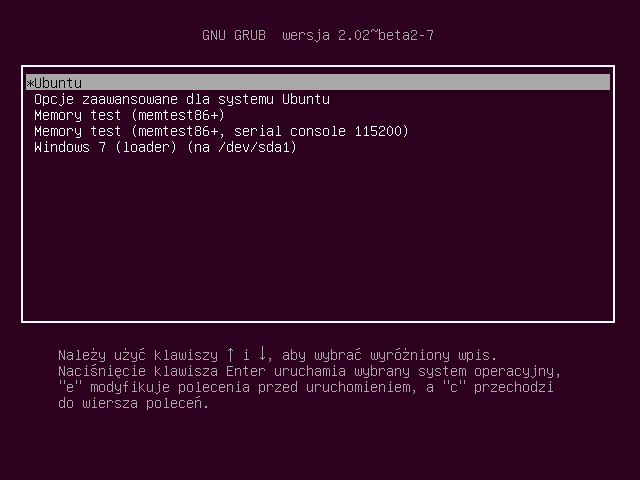
\includegraphics[width=\linewidth]{images/pierwsze_uruchomienie_grub.png}
\end{wrapfigure}

Po zainstalowaniu systemu Ubuntu twój komputer został zresetowany, zostałeś też poproszony o usunięcie nośnika instalacyjnego (pendrive, płyta DVD) z napędu. Jeżeli to wykonałeś to przy ponownym uruchomieniu komputera powinieneś zobaczyć ekran bardzo podobny do tego. Jest to GRUB (Grand Unified Bootloader), program rozruchowy zajmujący uruchomieniem systemu operacyjnego. Korzystając z GRUBA możesz wybrać, który system operacyjny ma zostać uruchomiony. Korzystając z klawiszy kursora na klawiaturze podświetl odpowiednią opcję i wciśnij Enter.
Jeżeli Ubuntu to jedyny system operacyjny zainstalowany na twoim komputerze to menu GRUBa nie wyświetli się. Zamiast niego Przez około sekundę widoczny będzie ciemnofioletowy ekran a następnie zostanie uruchomiony system Ubuntu. Aby w takiej sytuacji wejść do menu GRUBa wciśnij klawisz shift kiedy fioletowy ekran jest widoczny.

\textbf{Opcje zaawansowane dla systemu Ubuntu} to zestaw dodatkowych programów naprawczych i diagnostycznych dla systemu Ubuntu. Zostały one szerze opisane w rozdziale \ref{Rozwiązywanie problemów}

\textbf{Memorytest} to program służący do testowania pamięci operacyjnej komputera (RAM).
Opcja \textbf{Windows 7 Loader} uruchomi system operacyjny Windows 7.

\begin{flushright}
Wybierz \textbf{Ubuntu}, wciśnij klawisz Enter aby uruchomić Ubuntu.
\end{flushright}
\clearpage

        \subsection{Ekran logowania}
                W czasie ładowania się systemu operacyjnego będzie widoczne logo Ubuntu ze stopniowo wypełniającymi się kwardratami. Wciskając dowolny klawisz logo zostanie zastąpione szczególowym opisem tego co jest aktualnie wykonywane.

Kiedy proces uruchamiania systemu dobiegnie końca twoim oczom ukarze się ekran logowania systemu Ubuntu (jeżeli w czasie instalacji wybrałeś "Automatyczne Logowanie" to ten ekran zostanie pominięty i automatycznie zostaniesz przeniesiony do pulpitu).
\begin{center}
	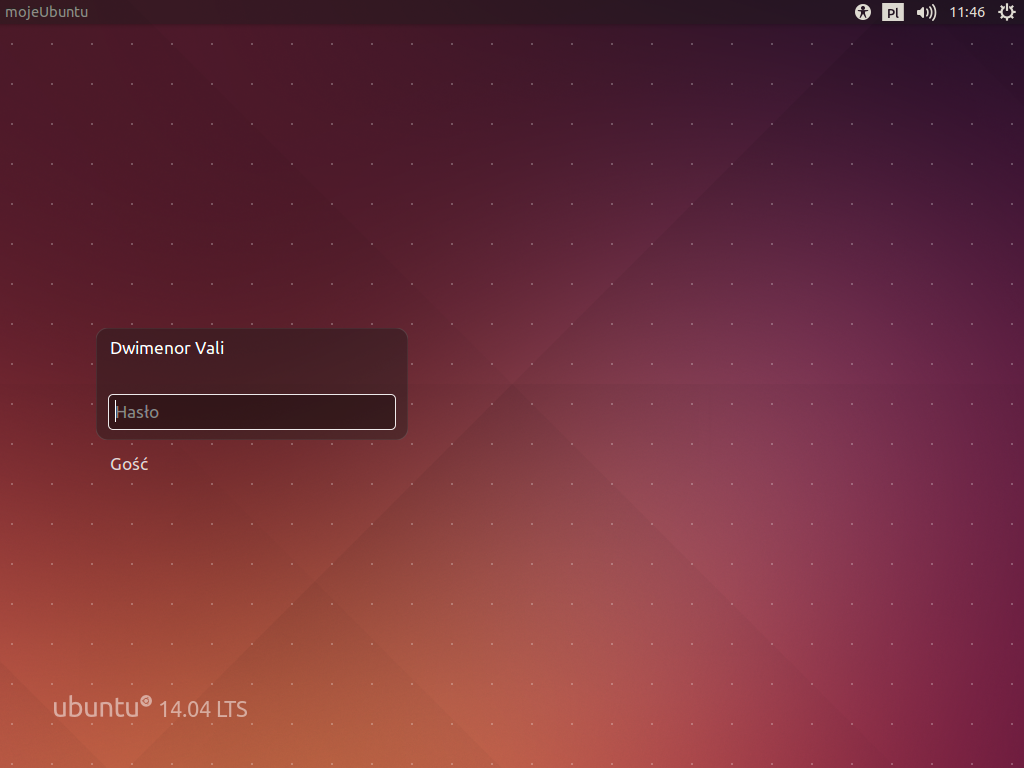
\includegraphics[scale=0.5]{images/greater.png}
\end{center}

\begin{enumerate}
\item Lista użytkowników systemu. Jeżeli w systemie jest więcej niż jeden użytkownik to z tej listy będzie można wybrać kto ma zostać zalogowany.
\item W to pole wpisz hasło aktualnie wybranego użytkownika.
\item Konto gość umozliwia zalogowanie się do systemu bez podawania hasła. Wszystkie zmiany wprowadzone przez gościa (np. utworzone pliki) zostaną utracone po zakończeniu sesji.
\item Nazwa systemu wybrana podczas instalacji.
\item Przyciski sterujące
\begin{description}
\item[
\includegraphics{images/ikony_dostempnosc2.png}]Dostepność - uruchomienie lupy, czytnika ekranowego lub klawiatury ekranowej.
\item[
\includegraphics{images/ikony_jezyk.png}]Język - pozwala zmienić układ klawiatury i metodę wprowadzania tekstu.
\item[
\includegraphics{images/ikony_dzwiek.png}]Ustawienia głośności i dźwięku.
\item[\textbf{11:46}] Zegar i kalendarz.
\item[
\includegraphics{images/ikony_zasilanie.png}]Wyłączenie lub ponowne uruchomienie komputera.
\end{description}
\end{enumerate}
\clearpage
        \subsection{Rzut oka na pulpit Ubuntu}
                \begin{wrapfigure}{R}{0.1\textwidth}
	
\includegraphics[width=\linewidth]{images/ikony_dash.png}
\end{wrapfigure}

Po zalogowaniu się do systemu na ekranie monitora zostanie wyświetlony pulpit systemu Ubuntu. Szczegółowy opis pulpitu znajduje się w kolejnym rozdziale \ref{pulpit_unity}: Pulpit Unity.

W tym rozdziale zajmiemy się najważniejszymi kwestiami związanymi z przygotowaniem systemu do codziennej pracy. Już teraz system jest gotowy, ale można wykonać kilka rzeczy, które uprzyjemnią obcowanie z Ubuntu. Aby sprawnie poruszać się po tej sekcji Przewodnika zapamiętaj tą ikonę.
        \subsection{Rzeczy do zrobienia po instalacji Ubuntu}
                \subsubsection{Aktualizacja systemu}
\label{rzeczy_do_zrobienia_po_instalacji}
\begin{wrapfigure}{R}{0.1\textwidth}
	\vspace{-10pt}
	
\includegraphics[width=\linewidth]{images/pierwsze_uruchomienie_aktualizacja1.png}
\end{wrapfigure}

Kliknij ikonę Dasha \includegraphics[scale=0.35]{images/ikony_dash.png} i wpisz \textcolor{ubuntu_orange}{Aktualizacje}. W trakcie wpisywania na ekranie wyników będą się pojawiały propozycje. Wybierz kolejno \menu{{Programy}>{Aktualizacje oprogramowania}}.
System sprawdzi, czy dostępne są aktualizacje dla twojego Ubuntu i wyświetli podsumowanie.
\begin{center}
	\includegraphics{images/pierwsze_uruchomienie_aktualizacja2.png}
\end{center}

Kliknij przycisk \textcolor{ubuntu_orange}{Zainstaluj}, aby zainstalować aktualizacje. Zostaniesz poproszony o podanie hasła w celu uwierzytelnienia. Każda operacja mająca wpływ na cały system wymaga potwierdzenia. Zapobiega to przypadkowemu uszkodzeniu systemu.
\begin{center}
	\includegraphics{images/unity_uwierzytelnienie.png}
\end{center}

Wpisz swoje hasło i potwierdź klawiszem Enter lub kliknij przycisk \textcolor{ubuntu_orange}{Uwierzytelnij}. Teraz rozpocznie się proces pobierania i instalacji aktualizacji. To może potrwać od kilkunastu sekund do kilku minut, w zależności od tego, jak długo system nie był aktualizowany.

Kiedy aktualizacja się zakończy, możesz zostać poproszony o ponowne uruchomienie komputera. Restart jest potrzebny tylko wtedy, gdy aktualizowane było jądro systemu lub sterowniki. Inne aktualizacje nie wymagają restartu komputera, a jedynie zaktualizowanego programu.

Później system będzie automatycznie sprawdzał, czy dostępne są aktualizacje, i powiadomi cię o tym.
\clearpage
\subsubsection{Instalacja spolszczenia}
\begin{wrapfigure}{R}{0.1\textwidth}
	\vspace{-10pt}
	\includegraphics[width=\linewidth]{images/pierwsze_uruchomienie_lang1.png}
\end{wrapfigure}

Jeżeli w trakcie instalacji systemu nie wybrałeś języka polskiego, lub nie miałeś połączenia z internetem, to tutaj dowiesz się, jak ściągnąć potrzebne paczki językowe i zainstalować odpowiednie oprogramowanie.
Kliknij ikonę Dasha \includegraphics[scale=0.35]{images/ikony_dash.png} i wpisz \textcolor{ubuntu_orange}{Języki}. System sprawdzi stan spolszczenia systemu i zaproponuje instalację dodatkowych paczek. Kliknij \textcolor{ubuntu_orange}{Zainstaluj}, a następnie potwierdź operację. Wpisz swoje hasło i potwierdź klawiszem Enter lub kliknij przycisk \textcolor{ubuntu_orange}{Uwierzytelnij}.

\begin{center}
	\vspace{-10pt}
	\includegraphics{images/pierwsze_uruchomienie_lang2.png}
\end{center}

Po instalacji niezbędnych paczek możesz jeszcze dla pewności kliknąć \textcolor{ubuntu_orange}{Zastosuj dla całego systemu}. W ten sposób będziesz pewny, że cały system zostanie spolszczony.
Jeśli zechcesz, aplikacja \textcolor{ubuntu_orange}{Języki} pozwoli ci później w łatwy sposób zainstalować i zmienić język systemu na każdy ze wspieranych przez społeczność Ubuntu.
\clearpage
\subsubsection{Instalacja dodatkowych sterowników}
\label{pierwsze_uruchomienie_aktualizacja_instalacja}
\begin{wrapfigure}{R}{0.1\textwidth}
	\vspace{-10pt}
	\includegraphics[width=\linewidth]{images/pierwsze_uruchomienie_driver1.png}
\end{wrapfigure}

Prawdopodobnie nie wszystkie sterowniki zostały włączone podczas instalacji Ubuntu. Aby się upewnić, że sprzęt jest prawidłowo obsługiwany, kliknij ikonę Dasha \includegraphics[scale=0.35]{images/ikony_dash.png} i wpisz \textcolor{ubuntu_orange}{Sterowniki}. Z wyświetlonych wyników wybierz ,,Aktualizacje i sterowniki''. W otwartym oknie przejdź do zakładki ,,Dodatkowe sterowniki''. Poczekaj chwilę, aż system zbierze dane o twoim komputerze i porówna je z bazą danych sterowników. Następnie będziesz mógł wybrać, który sterownik z wyświetlonej listy powinien zostać użyty.
\begin{center}
	\includegraphics[width=\linewidth]{images/pierwsze_uruchomienie_driver2.png}
\end{center}

Zmiana sterownika wymaga potwierdzenia. Wpisz swoje hasło i potwierdź klawiszem Enter lub kliknij przycisk \textcolor{ubuntu_orange}{Uwierzytelnij}. Więcej o wyborze sterownika przeczytasz w rozdziale \ref{sterowniki},,Sterowniki''.
\clearpage
\subsubsection{Instalacja dodatków}
\label{ubuntu-restricted-extras}
\begin{wrapfigure}{R}{0.1\textwidth}
	\vspace{-10pt}
	\includegraphics[width=\linewidth]{images/pierwsze_uruchomienie_dodatki1.png}
\end{wrapfigure}

Na koniec warto zainstalować kilka dodatkowych pakietów oprogramowania. Kliknij ikonę Dasha \includegraphics[scale=0.35]{images/ikony_dash.png} i wpisz \textcolor{ubuntu_orange}{Centrum Oprogramowania}. Z wiersza \textcolor{ubuntu_orange}{Programy} wybierz \textcolor{ubuntu_orange}{Centrum Oprogramowania Ubuntu}. W prawym górnym rogu nowo otwartego okna znajduje się pole wyszukiwania. Wpisz w nim \textcolor{ubuntu_orange}{Ograniczone dodatki Ubuntu} i wciśnij Enter. Poczekaj, aż odnaleziona zostanie ta paczka. Z listy wybierz \textcolor{ubuntu_orange}{Ubuntu restricted extras} i kliknij \textcolor{ubuntu_orange}{Zainstaluj}. Instalacja oprogramowania wymaga uwierzytelnienia. Wpisz swoje hasło i potwierdź klawiszem Enter lub kliknij przycisk \textcolor{ubuntu_orange}{Uwierzytelnij}.
\begin{center}
	\includegraphics[width=\linewidth]{images/pierwsze_uruchomienie_dodatki2.png}
\end{center}

Paczka \textcolor{ubuntu_orange}{ubuntu-restricted-extras} zawiera:
\begin{itemize}
\item wszystkie możliwe kodeki audio/wideo;
\item odtwarzcacz Flash;
\item fonty True Type (np. Times New Roman).
\end{itemize}
W podobny sposób wyszukaj i zainstaluj programy \textcolor{ubuntu_orange}{openjdk-7-jre} (Java, potrzebna do wielu popularnych programów), \textcolor{ubuntu_orange}{unzip} (obsługa archiwów zip), \textcolor{ubuntu_orange}{unace} (windowsowe archiwa ace) i \textcolor{ubuntu_orange}{p7zip-full} (obsługa archiwów w formacie 7z/lzma).
\clearpage

\section{Pulpit Ubuntu Unity}
        \label{pulpit_unity}
        \subsection{Pulpit}
        		\begin{center}
	\includegraphics[scale=0.4]{images/unity_desktop.png}
\end{center}

Po zalogowaniu się do systemu Twoim oczom ukaże się Pulpit. Widać na nim trzy elementy: przestrzeń roboczą wypełniającą większą część ekranu oraz dwa panele. Panel poziomy, zwany \textbf{panelem menu}, umieszczony na górze ekranu. Panel pionowy to \textbf{Launcher}, zlokalizowany jest po lewej stronie ekranu.
\clearpage

\subsubsection{Zmiana tła pulpitu}
Aby zmienić tło pulpitu (inaczej: tapetę) kliknij \textbf{prawym przyciskiem myszy} na wolnej przestrzeni roboczej i z menu kontekstowego wybierz "Zmień tło pulpitu"

\begin{wrapfigure}{r}{0.5\textwidth}
                \includegraphics[width=\linewidth]{images/unity_zmiana_tapety.png}
\end{wrapfigure}

Z listy zaznaczonej jako (1) możesz wybrać jedną z gotowych tapet. Kliknij na przycisk + (2) aby otworzyć menadźer plików i wskazać inny plik graficzny na dysku twardym. Plik ten zostanie użyty jako tapeta.

W tym oknie możesz też dokonać pewnych modyfikacji środowiska graficznego Unity. Zachęcamy do eksperymentów. Wszelkie zmiany są wprowadzane na żywo.
\clearpage

       
        \subsection{Panel Menu}
        		\textcolor{ubuntu_orange}{Panel menu} łączy w sobie kilka funkcji i to, co od razu rzuca się w oczy, to umieszczony po prawej stronie \textcolor{ubuntu_orange}{obszar powiadamiania}, zwany inaczej obszarem wskaźników.

\begin{center}
	\includegraphics[width=\linewidth]{images/unity_menu_bar.png}
\end{center}

Część wskaźników widoczna jest zaraz po zainstalowaniu systemu, inne można włączyć dodatkowo. Niektóre aplikacje po zainstalowaniu dodają, lub umożliwiają dodanie własnych wskaźników do obszaru powiadamiania. Najczęściej stosowane i domyślnie dostępne w Unity wskaźniki, to:
\begin{description}
\item[\includegraphics{images/unity_wskaznik_klawiatura.png}]\textcolor{ubuntu_orange}{Wskaźnik klawiatury} --- informuje o aktualnie używanym układzie klawiatury. Klikając go możesz zmienić układ klawiatury.
\item[\includegraphics{images/unity_wskaznik_siec.png}]\textcolor{ubuntu_orange}{Wskaźnik połączeń sieciowych} --- informuje o stanie połączenia z siecią. Kliknięcie wywołuje opcje modyfikacji połączenia z internetem.
\item[\includegraphics{images/unity_wskaznik_wiadomosci.png}]\textcolor{ubuntu_orange}{Wskaźnik wiadomości} --- informuje o przychodzących wiadomościach. Ten wskaźnik integruje się z komunikatorami internetowymi i zmienia kolor, gdy otrzymasz nową wiadomość. Pozwala także sterować komunikatorem, np. zmienić status lub wywołać okno główne.
\item[\includegraphics{images/unity_wskaznik_dzwiek.png}]\textcolor{ubuntu_orange}{Wskaźnik ustawień dźwięku} --- informuje o głośności wyjścia audio. Jeżeli kursor myszy znajduje się nad tym wskaźnikiem, to poruszając kółkiem myszy możesz zmieniać głośność. Kliknięcie wskaźnika otwiera menu ustawień dźwięku oraz menu sterownia odtwarzaczem muzyki (pozwala np. go uruchomić lub zatrzymać, zmienić utwór, wyświetlić okładkę i informacje o aktualnie odtwarzanym pliku,a także włączyć listę odtwarzania).
\item[\includegraphics{images/unity_wskaznik_zasilanie.png}]\textcolor{ubuntu_orange}{Wskaźnik zasilania i poziomu akumulatora} --- informuje o stanie stanie naładowania akumulatora oraz o dostępnym zasilaniu (akumulator/sieć). Ten wskaźnik nie jest wyświetlany, jesli komputer nie ma baterii. Kliknięcie wskaźnika otwiera menu zasilania.
\item[\includegraphics{images/unity_wskaznik_zegar.png}]\textcolor{ubuntu_orange}{Zegar} --- wyświetla aktualną datę i czas. Kliknięcie otwiera kalendarz.
\item[\includegraphics{images/unity_wskaznik_system.png}]\textcolor{ubuntu_orange}{Wskaźnik sesji} --- po kliknięciu wyświetla menu systemowe, pozwalające wyłączyć/zrestartować komputer, wyświetlić informacje o systemie, przełączyć użytkownika lub otworzyć narzędzie konfiguracji systemu.
\end{description}

\label{unity_menu_bar}
W Unity pasek menu aplikacji (\menu{Plik}, \menu{Edycja}, \menu{Narzędzia}, itd) nie jest umieszczony na belce okna, lecz domyślnie wyświetlany jest w lewej części panelu menu. Po uruchomieniu dowolnego programu pasek menu zawiera jedynie nazwę aktualnie aktywnego okna:

\begin{center}
	\includegraphics[width=\linewidth]{images/unity_menu_bar2.png}
\end{center}

Pasek menu jest wyświetlany, gdy kursor myszy znajdzie się nad panelem menu:

\begin{center}
	\includegraphics[width=\linewidth]{images/unity_menu_bar3.png}
\end{center}

Umieszczenie paska menu na panelu ma swoje plusy w przypadku urządzeń z ekranem ograniczonym niską rozdzielczością. Tak zwane \textcolor{ubuntu_orange}{Global Menu} pozwala lepiej wykorzystać miejsce dostępne w pionie.

        \subsection{Launcher}
        		Pasek umieszczony po lewej stronie ekranu nosi nazwę Launchera (ang: \textcolor{ubuntu_orange}{Wyzwalacz}). Launcher umożliwia przechowywanie skrótów do ulubionych i najczęściej używanych aplikacji, dostęp do uruchomionych programów, zamontowanych urządzeń (pamięć USB/SD, zewnętrzne dyski twarde, CD/DVD) oraz kosza. Uruchomiona aplikacja na czas pracy umieszcza w Launcherze swoją ikonę.

\subsubsection{Uruchamianie programów z Launchera}
\begin{wrapfigure}{l}{0.1\textwidth}
	\vspace{-10pt}
	\includegraphics[width=\linewidth]{images/unity_launcher_programy.png}
\end{wrapfigure}

Aby uruchomić program bezpośrednio z Launchera, wystarczy pojedyncze kliknięcie ikony wybranego programu lewym przyciskiem myszy. Uruchomione programy mają podświetlone ikony oraz niewielki trójkącik po lewej stronie. Aby uruchomić kolejną kopię programu, kliknij jego ikonę lewym przyciskiem myszy, trzymając wciśnięty klawisz \keys{Shift}.

Liczba trójkątów po lewej stronie programu oznacza ilość otwartych kopii danego programu. Jak łatwo się domyślić, gdy ikona nie ma żadnego trójkącika, to program jest wyłączony. Program, którego aktualnie używamy (aktywne okno), jest oznaczony trójkącikiem po prawej stronie ikony.

Na rysunku obok widzimy ikonę programu Pliki (menadżer plików Nautilus), który jest uruchomiony jeden raz. Tło ikony jest podświetlone.

Ikona przeglądarki internetowej Firefox ma trzy trójkąty po lewej. Oznacza to, że została uruchomiona w trzech osobnych instancjach. Jedna z kopii Firefoksa jest akurat w użyciu, co sygnalizuje trójkącik po prawej. Tło ikony jest podświetlone. Trzecia ikona na rysunku (skrót do procesora tekstu LibreOffice Writer) jest nieaktywna. Ten program nie jest aktualnie uruchomiony.

\subsubsection{Zarządzanie otwartymi oknami}
Kliknięcie ikony uruchomionego programu lewym przyciskiem myszy przenosi do otwartego okna. Jeżeli dany program ma więcej niż jedną instancję, to pokazane zostaną miniatury wszystkich jego okien. Klikając lewym przyciskiem myszy możesz wybrać, o które okno ci chodzi. 

Kółkiem myszy możesz przełączać pomiędzy instancjami programu. Umieść kursor myszy nad ikoną aplikacji i poruszaj kółkiem myszy w górę lub w dół, aby przejść do następnej/poprzedniej instancji programu.

\subsubsection{Zmiana położenia ikon}
\begin{wrapfigure}[5]{l}{0.25\textwidth}
	\vspace{-10pt}
	\includegraphics[width=\linewidth]{images/unity_launcher_zmiana_polozenia_ikon.png}
\end{wrapfigure}

Zawartość Launchera, poza ikoną Dasha oraz kosza, może być dowolnie modyfikowana. Aby zmienić położenie ikony na panelu, umieść kursor myszy nad ikoną, wciśnij i przytrzymaj lewy przycisk myszy. Kiedy ikona zostanie odczepiona od Launchera, przesuń ją na wybrane przez siebie miejsce i puść przycisk myszy.

\subsubsection{Dodawanie ikon do Launchera}
Skrót programu można dodać do Launchera na dwa sposoby. Pierwszy wykorzystuje okno Dasha (o którym będzie później). Aby dodać ikonę do paska bezpośrednio z Dasha, należy odszukać program i przeciągnąć jego ikonę w dowolne miejsce Launchera.

Druga metoda polega na uruchomieniu programu. Następnie należy kliknąć prawym przyciskiem myszy ikonę uruchomionego programu i z menu kontekstowego, które się pojawi, wybrać \textcolor{ubuntu_orange}{Dodaj do panelu uruchamiania}.

\subsubsection{Usuwanie ikon z Launchera}
Ikonę z paska można usunąć na dwa sposoby. Chwyć ikonę kursorem myszy i przenieś ją do kosza lub, po naciśnięciu ikony prawym przyciskiem myszy, z menu kontekstowego wybierz \textcolor{ubuntu_orange}{Usuń z panelu uruchamiania}.

\subsubsection{Szybka Lista menu kontekstowego (QuickList)}
QuickList (Szybka Lista) to jedna z ciekawszych funkcji Launchera. Po kliknięciu prawym przyciskiem myszy ikony programu w Launcherze pojawia się menu kontekstowe, w którym można umieścić różne polecenia. Na poniższej ilustracji widać dwa przykłady. Po lewej mamy menu kontekstowe Dasha, zawierające skróty do zainstalowanych soczewek (omówionych w kolejnym rozdziale). Po prawej widać menu kontekstowe menadżera plików, zawierające skróty do najważniejszych katalogów użytkownika. Przeglądarka internetowa Firefox pozwoli dodatkowo uruchomić okno anonimowego przeglądania.

\begin{center}
	\includegraphics[width=\linewidth]{images/unity_launcher_quicklist.png}
\end{center}



        \subsection{Dash}
        		\begin{center}
	\includegraphics[scale=0.5]{images/unity_pulpit_dash.png}
\end{center}

Dash jest potężnym narzędziem w Unity, które w szybki sposób pozwala nam na dostęp i wyszukiwanie programów, plików oraz dodatkowych informacji przechowywanych nie tylko w naszym komputerze (zainstalowane programy, ostatnio używane dokumenty, zakładki i ostatnio odwiedzone strony i inne), ale również informacji dostępnych w sieci (Twitter, Facebook, Google Docs, Youtube, Wikipedia, Amazon i inne). Wyniki wyszukiwania w zewnętrznych serwisach dopasowane są do wyszukiwanej frazy i zwracane są w oknie Dasha. Jeżeli przejmujesz się tym, że szukana fraza przesyłana do Internetu, to funkcjonalność ta może zostać wyłączona w Ustawieniach systemowych w oknie \textbf{Prywatność i bezpieczeństwo.}

Dash można porównać do Menu Start z systemu Microsoft Windows XP/Vista/7 lub do ekranu startowego w Windows 8. Odpowiednikiem Dasha w systemie OS X jest Launchpad.

\begin{wrapfigure}{l}{0.1\textwidth}
                \includegraphics[width=\linewidth]{images/ikony_dash.png}
\end{wrapfigure}

Ikona Dasha umieszczona jest na pierwszej pozycji na pasku Launchera – jest ona dość charakterystyczna i zawiera logo Ubuntu. Po naciśnięciu na ikonę Dasha naszym oczom ukaże się jego przezroczyste okno, które w swojej środkowej części okna wyświetla dwie grupy: ostatnio uruchomionych programów oraz ostatnio przeglądanych i pobranych plików oraz katalogów, a także wyszukiwanych informacji. W górnej części Dasha znajduje się pasek wyszukiwania, który nie tylko pozwala przeszukiwać zasoby komputera, ale pozwala również wyszukiwać i przeglądać informacje z popularnych serwisów w sieci. 

\begin{wrapfigure}{l}{0.2\textwidth}
                \includegraphics[width=\linewidth]{images/unity_dash_max.png}
\end{wrapfigure}

Dash po uruchomieniu zajmuje pewien obszar ekranu. Okno to można powiększyć do pełnego rozmiaru ekranu – służy do tego przycisk maksymalizacji w lewym górnym rogu, który jest widoczny, gdy Dash jest wywołany.\\
Wyszukiwanie w pasku jest dynamiczne i rezultaty zmieniają się podczas wpisywania tekstu. Wyniki w Dashu można filtrować. Służy do tego nie tylko przycisk Filtrowania wyników, ale również domyślnie włączone soczewki (Lenses).
\clearpage

\subsubsection{Soczewki (Lenses)}
\begin{center}
	\includegraphics[scale=0.5]{images/unity_dash_lenses.png}
\end{center}

Domyślnie w systemie dostępnych jest siedem soczewek i umieszczone są one na dole okna Dasha. Aktualnie wybrana soczewka jest jaśniejsza od pozostałych oraz ma nas sobą niewielki trójkącik. Soczewki służą do ograniczania wyników wyszukiwania do konkretnych kategorii.
\begin{description}
\item[\includegraphics{images/unity_dash_lens_home.png}] \textbf{Soczewka domowa} zawiera wszystkie wyniki wyszukiwania. 
\item[\includegraphics{images/unity_dash_lens_programy.png}] \textbf{Soczewka programów} zawiera wyniki wyszukiwania programów.
\item[\includegraphics{images/unity_dash_lens_pliki.png}] \textbf{Soczewka plików} zawiera wyniki wyszukiwania w plikach i katalogach.
\item[\includegraphics{images/unity_dash_lens_video.png}] \textbf{Soczewka filmów} zawiera wyniki wyszukiwania filmów.
\item[\includegraphics{images/unity_dash_lens_audio.png}] \textbf{Soczewka muzyki} zawiera wyniki wyszukiwania muzyki.
\item[\includegraphics{images/unity_dash_lens_photo.png}] \textbf{Soczewka zdjęć} zawiera wyniki wyszukiwania w fotografiach.
\item[\includegraphics{images/unity_dash_lens_social.png}] \textbf{Soczewka społecznościowa} zawiera wyniki wyszukiwania w serwisach społecznościowych do których jesteś zalogowany.
\end{description}
\clearpage
Soczewka domowa ma wiele zastosowań i oprócz wcześniej wspomnianych możliwości, możemy ją wykorzystać do wyszukania informacji na przykład w Wikipedii, Google lub możemy wyszukać informacji na temat pogody w naszym regionie.
\begin{center}
	\includegraphics[scale=0.75]{images/unity_dash_wyszukiwanie.png}
\end{center}
\clearpage
Aby uzyskać więcej informacji, nie trzeba od razu otwierać wyniku. Naciśnięcie prawym przyciskiem myszy którymś z wyników wyszukiwania, poda nam więcej informacji.
\begin{center}
	\includegraphics[scale=0.75]{images/unity_dash_wyszukiwanie2.png}
\end{center}
\clearpage
Wyniki wyszukiwania można zawęzić do konkretnych źródeł wykorzystując do tego przycisk Filtrowania wyników. Podobnie jest w przypadku wyszukiwania informacji z wykorzystaniem pozostałych soczewek.
\begin{center}
	\includegraphics[scale=0.75]{images/unity_dash_wyszukiwanie3.png}
\end{center}

W Ubuntu nie jesteśmy limitowani jedynie zainstalowanymi soczewkami. Wiele serwisów Internetowych udostępnia swoje własne soczewki, które można w łatwy sposób doinstalować i korzystać z nich w ten sam sposób, jak z domyślnie dostępnych.
%TODO opisać instalację soczewki.
\clearpage



        	\subsection{Obszary robocze}
        		Obszary robocze, powszechnie zwane wirtualnymi pulpitami, pozwalają w łatwy sposób zarządzać i grupować programy. Dzięki temu, przy dużej liczbie otwartych okien, w łatwy sposób możemy zredukować zatłoczenie i usprawnić nawigację po pulpicie. Dla przykładu, w jednym obszarze roboczym możemy przeglądać zasoby Internetu, a w drugim lub trzecim możemy mieć uruchomiony program do przeglądania multimediów oraz tworzyć dokument w programie biurowym.

Domyślnie Ubuntu daje dostęp do czterech obszarów roboczych, ale zaraz po instalacji ta opcja nie jest włączona. Aby móc korzystać z dodatkowych obszarów roboczych, kliknij ikonę systemową \includegraphics{images/ikony_zasilanie.png} na panelu menu (w prawym górnym rogu) i wybierz \menu{{Ustawienia Systemu}>{Osobiste}>{Wygląd}>{Zachowanie}>{Uaktywnij obszary robocze}}.

\begin{wrapfigure}{l}{0.05\textwidth}
	\vspace{-10pt}
	\includegraphics[width=\linewidth]{images/ikony_obszary_robocze.png}
\end{wrapfigure}

Po zaznaczeniu dodatkowych obszarów roboczych na pasku Launchera pojawi się dodatkowa ikona, służąca do przełączania pomiędzy obszarami roboczymi: \textcolor{ubuntu_orange}{Przełącznik obszarów roboczych}.
\clearpage
Domyślnie w Ubuntu masz do dyspozycji cztery wirtualne pulpity, ułożone w siatkę 2x2. Po naciśnięciu ikony obszarów roboczych na ekranie pojawia się siatka czterech pulpitów. Pomiędzy obszarami roboczymi możesz się też przemieszczać za pomocą następujących skrótów klawiszowych:
\begin{itemize}
\item \keys{CTRL + ALT + \arrowkeyright} przenosi do obszaru roboczego po prawej;
\item \keys{CTRL + ALT + \arrowkeyleft} przenosi do obszaru roboczego po lewej;
\item \keys{CTRL + ALT + \arrowkeyup} przenosi do obszaru roboczego na górze;
\item \keys{CTRL + ALT + \arrowkeydown} przenosi do obszaru roboczego na dole.
\end{itemize}

        	\subsection{Zarządzanie oknami}
        		\begin{center}
	\vspace{-10pt}
	\includegraphics[width=\linewidth]{images/unity_okno_belka.png}
\end{center}

W Ubuntu elementy sterujące okna (przyciski zamykania, minimalizacji i maksymalizacji) znajdują się po lewej stronie. Również tytuł okna znajduje się nie na środku, a jest przesunięty ku lewej.

\subsubsection{Elementy sterujące oknami}
\begin{description}
\item[\includegraphics{images/unity_okno_exit.png}] Zamknij okno.
\item[\includegraphics{images/unity_okno_min.png}] Minimalizuj okno do paska Launchera.
\item[\includegraphics{images/unity_okno_max.png}] Maksymalizuj okno do rozmiaru pulpitu. Belka okna, zawierająca opisywane przyciski oraz tytuł, zostanie zintegrowana z panelem menu.
\end{description}

\subsubsection{Przenoszenie i zmiana rozmiaru okna}
Po kliknięciu lewym przyciskiem myszy belki tytułowej okna i przytrzymaniu, możemy je przenieść w dowolne miejsce na pulpicie. Okno można również przenieść przytrzymując przycisk \keys{Alt} --- wówczas wystarczy kliknąć lewym przyciskiem myszy i przytrzymać w dowolnym miejscu okna, które chcemy przenieść.

Aby zmienić rozmiar okna, kursor myszy należy umieścić nad wybraną krawędzią lub rogiem okna. Domyślny kursor zmieni się wówczas w dwustronną strzałkę, zwaną kursorem rozszerzania. Przytrzymanie przycisku myszy, gdy aktywny jest kursor rozszerzania, pozwoli na zmianę rozmiaru i kształtu okna.

\subsubsection{Przełączanie pomiędzy otwartymi oknami}
W Ubuntu jest wiele sposobów na przełączanie pomiędzy otwartymi programami. Można wykorzystać mysz i kliknąć w dowolnym miejscu otwartych okien. Można wykorzystać ikony otwartych okien na pasku Launchera. Można również wykorzystać kombinację klawiszy \keys{Alt + Tab}.

Gdy mamy otwarte wiele okien, przytrzymanie przycisku \keys{Alt} i wielokrotne naciskanie przycisku \keys{Tab} pozwala wybrać, które okno chcemy aktywować. Domyślnie przełączane w ten sposób są tylko okna z aktywnego obszaru roboczego. Korzystając z kombinacji \keys{Super + Tab} możemy przełączać pomiędzy kolejnymi ikonami na pasku Launchera.

\subsubsection{Ukrywanie wszystkich okien --- pokaż pulpit}
Aby ukryć wszystkie okna, nie trzeba ich, jedno po drugim, minimalizować. Można skorzystać ze skrótu \keys{Ctrl + Super + d}. Jego użycie spowoduje ukrycie wszystkich otwartych okien. Ponowne zastosowanie tego skrótu przywróci otwarte okna.

\begin{wrapfigure}{l}{0.05\textwidth}
	\vspace{-10pt}	
	\includegraphics[width=\linewidth]{images/ikony_pokaz_pulpit.png}
\end{wrapfigure}

W Ubuntu można również aktywować ikonę \textcolor{ubuntu_orange}{Pokaż pulpit}. Aby to zrobić, kliknij ikonę systemową \includegraphics{images/ikony_zasilanie.png} na panelu menu (w prawym górnym rogu) i wybierz \menu{{Ustawienia systemu}>{Osobiste}>{Wygląd}>{Zachowanie}>{Umieść ikonę ,,Pokaż pulpit'' na pasku Launchera}}.

\subsubsection{Przenoszenie otwartych okien pomiędzy obszarami roboczymi}
Przenoszenie otwartych okien pomiędzy obszarami roboczymi jest również dość proste i intuicyjne. Wystarczy uruchomić podgląd obszarów roboczych i przeciągnąć otwarte okno z jednego do drugiego.

\begin{center}
	\includegraphics[width=\linewidth]{images/unity_okno_przenoszenie1.png}
\end{center}

\begin{center}
	\includegraphics[width=\linewidth]{images/unity_okno_przenoszenie2.png}
\end{center}

\begin{center}
	\includegraphics[width=\linewidth]{images/unity_okno_przenoszenie3.png}
\end{center}

Aby przenieść okno do innego obszaru roboczego, można również kliknąć belkę tytułową otwartego okna prawym przyciskiem myszy i z menu kontekstowego wybrać którąś z opcji:
\begin{itemize}
\item \textcolor{ubuntu_orange}{Przenieś do lewego obszaru}, gdy chcemy przenieść okno do lewego obszaru.
\item \textcolor{ubuntu_orange}{Przenieś do prawego obszaru}, gdy chcemy przenieść okno do prawego obszaru.
\item \textcolor{ubuntu_orange}{Przenieś do dolnego obszaru}, gdy chcemy przenieść okno do dolnego obszaru.
\item \textcolor{ubuntu_orange}{Przenieś do górnego obszaru}, gdy chcemy przenieść okno do górnego obszaru.
\item \textcolor{ubuntu_orange}{Przenieś do innego obszaru}, gdy chcemy wybrać, do którego konkretnie obszaru chcemy przenieść okno.
\end{itemize}

\subsubsection{Zawsze na wierzchu}
Niekiedy okno jakieś aplikacji chcemy mieć zawsze widoczne na pierwszym planie, pomimo tego, że aktualnie pracujemy w innym oknie. Aby utrzymać okno zawsze widoczne na pierwszym planie, należy kliknąć belkę tytułową okna prawym przyciskiem myszy i z menu kontekstowego wybrać opcję \textcolor{ubuntu_orange}{Zawsze na wierzchu}.

\subsubsection{Zawsze na widocznym obszarze roboczym}
W Ubuntu dostępna jest jeszcze jedna bardzo przydatna funkcja, związana z zachowaniem okien. Gdy wykorzystujemy obszary robocze, czasem chcemy, by okno aplikacji zawsze pojawiało się na tym obszarze roboczym, który jest używany. W tym celu należy kliknąć belkę tytułową okna prawym przyciskiem myszy i z menu kontekstowego wybrać opcję \textcolor{ubuntu_orange}{Zawsze na widocznym obszarze roboczym}.

        \subsection{HUD - Heads-Up Display}
    		    	Spamiętanie wszystkich skrótów klawiaturowych może być trudne, zwłaszcza gdy mamy do czynienia z programami, które mają ich wiele do dyspozycji. Często też niektóre programy nie posiadają przycisków w oknie programu lub skrótów do pewnych funkcji, ukrytych gdzieś głęboko za którymś z~przycisków na pasku menu. Często jest tak, że pamiętamy nazwę funkcji, ale już nie bardzo miejsce, w którym się ona znajduje. Tu z pomocą przychodzi \textcolor{ubuntu_orange}{HUD} (Heads-up Display).

HUD jest silnie zintegrowanym narzędziem, które przy wykorzystaniu klawiatury pozwala dotrzeć nie tylko do najczęściej wykorzystywanych funkcji programu, ale również tych, o których często zapominamy, gdyż są zaszyte gdzieś głęboko. Przykładowe wykorzystanie HUD-a do skopiowania pliku:

\begin{center}
	\includegraphics[width=\linewidth]{images/unity_hud1.png}
\end{center}

Inny przykład: powiedzmy, że tworzymy dokument w programie OpenOffice Writer i potrzebujemy wstawić obiekt, czy formułę. Osobie, która z programu korzysta rzadko, znalezienie tej funkcji może zająć dłuższą chwilę. Z wykorzystaniem HUD-a jest to kwestia wpisania słowa ,,formuła'' i wybrania odpowiedniej opcji w oknie wyników wyszukiwania.

        \subsection{Nautilus - Menadżer plików}
			\begin{wrapfigure}{l}{0.1\textwidth}
	\vspace{-10pt}
	\includegraphics[width=\linewidth]{images/ikony_pliki.png}
\end{wrapfigure}

Menadżer plików jest programem służącym do przeglądania zawartości katalogów. W Ubuntu menadźer plików nazywa się \textcolor{ubuntu_orange}{Nautilus} i jest odpowiednikiem programu \textcolor{ubuntu_orange}{Eksplorator Windows} z systemów Windows oraz \textcolor{ubuntu_orange}{Finder} z Mac OX X. Na pasku Launchera Nautilus domyślnie jest drugą dostępną ikoną. 

Program Pliki po uruchomieniu wyświetla zawartość katalogu domowego użytkownika, w którym to użytkownik przechowuje swoje osobiste pliki. Każdy użytkownik ma swój oddzielny katalog domowy, którego nazwa odpowiadania nazwie użytkownika. Po utworzeniu konta w katalogu domowym automatycznie utworzone są katalogi Dokumenty, Muzyka, Obrazy, Pobrane, Publiczny, Pulpit, Szablony, Wideo. Użytkownik nie jest ograniczony jedynie do tych katalogów i bez problemu w katalogu domowym może dodać więcej katalogów oraz plików.

\begin{center}
	\includegraphics[width=\linewidth]{images/programy_nautilus.png}
\end{center}

W oknie menadżera plików widzimy:
\begin{enumerate}[label=\protect\circled{\arabic*}]
\item Przyciski \textcolor{ubuntu_orange}{Do tyłu} i \textcolor{ubuntu_orange}{Do przodu}.
\item Aktualne położenie.
\item Zawartośc aktualnego katalogu.
\item Pasek ze skrótami do najważniejszych miejsc.
\end{enumerate}

Menadżer plików w lewym panelu będzie też wyświetlał podłączone urządzenia (pendrive, karty SD, płyty włożone do czytników optycznych) oraz udziały sieciowe (inne podłączone komputery). Pozycja \textcolor{ubuntu_orange}{Komputer} przenosi do początku systemu plików (katalog /)

Do nawigacji w pasku narzędzi oraz lewym panelu wykorzystywane jest pojedyncze kliknięcie lewym przyciskiem myszy. W prawym panelu pliki oraz katalogi domyślnie otwieramy dwukrotnym szybkim przyciśnięciem lewego przycisku myszy. W przypadku otwarcia pliku, Ubuntu rozpozna typ pliku i automatycznie spróbuje przypisać odpowiednią dla danego pliku aplikację. Czasami, system może nie rozpoznać typu pliku lub może zajść potrzeba otwarcia pliku wykorzystując inny program. W takich wypadkach, po dwukrotnym kliknięciu na pliku system zapyta nas, który program z zainstalowanych w systemie chcemy wykorzystać. Możemy również nacisnąć prawym przyciskiem myszy na pliku i z menu kontekstowego wybrać Otwórz za pomocą i wybrać z listy dostępnych programów lub samemu wybrać inny.

Najważniejsze katalogi w folderze użytkownika:
\begin{itemize}
\item \textcolor{ubuntu_orange}{Pulpit} --- wszystkie pliki i foldery umieszczone w tym katalogu zostaną wyświetlone na pulpicie.
\item \textcolor{ubuntu_orange}{Dokumenty} --- katalog na dokumenty, pliki tekstowe, arkusze kalkulacyjne itp.
\item \textcolor{ubuntu_orange}{Muzyka} --- katalog z plikami muzycznymi. Odtwarzacze muzyki będą szukać plików do odtwarzania najpierw w tym folderze.
\item \textcolor{ubuntu_orange}{Wideo} --- katalog z plikami wideo.
\item \textcolor{ubuntu_orange}{Obrazy} --- katalog z fotografiami.
\item \textcolor{ubuntu_orange}{Pobrane} --- katalog na pliki pobrane z internetu. przeglądaki internetowe domyślnie będą zapisywać pobrane pliki w tym katalogu.
\end{itemize}

\subsubsection{Tworzenie nowych katalogów}
Tworzenie nowych katalogów niczym nieróżni się się od metod, które dostępne są w innych systemach. Zwyczajnie wystarczy nacisnąć prawym przyciskiem myszy na wolnej przestrzeni w oknie programu (ta metoda również zadziała na naszym pulpicie) i z menu kontekstowego wybrać opcję \textcolor{ubuntu_orange}{Nowy katalog}. Można również wykorzystać w tym celu panel menu i wybrać \menu{Plik>{Nowy katalog}}. Można również wykorzystać skrót klawiaturowy \keys{Shift + CTRL + n}.

\subsubsection{Ukryte pliki i katalogi}
Ubuntu, jak każdy inny Linux, umożliwia tworzenie ukrytych plików oraz katalogów. Aby ukryć plik lub katalog, wystarczy w jego nazwie na samym początku wstawić znak kropki (.). Gdy chcemy uzyskać dostęp do ukrytych plików lub katalogów, należy z panelu menu wybrać \menu{Widok>Wyświetlanie ukrytych plików} lub skorzystać ze skróty klawiaturowego \keys{CTRL + h}.

UWAGA: Wyświetlenie ukrytych plików w katalogu domowym użytkownika wyświetli wiele dodatkowych plików oraz katalogów, które w większości przypadków przechowują ustawienia dla wielu programów użytkownika, wyglądu konta użytkownika oraz zachowań na koncie użytkownika. Niewłaściwe obchodzenie się z tymi plikami, może mieć negatywne skutki. Zaleca się zatem dodatkową ostrożność.

\subsubsection{Kopiowanie i przenoszenie plików oraz katalogów}
Ubuntu, jak każdy inny system również umożliwia kopiowanie i przenoszenie plików oraz katalogów z jednego miejsca do innego. Aby plik lub katalog skopiować lub przenieść z jednego miejsca do innego, trzeba go najpierw zaznaczyć, a następnie nacisnąć na obiekcie prawym przyciskiem myszy i wybrać z menu kontekstowego skopiuj (w przypadku, gdy chcemy go utworzyć kopię) lub wytnij (w przypadku, gdy plik chcemy przenieść), a następnie przechodzimy do katalogu, w którym plik chcemy umieścić i w wolnym miejscu naciskamy prawym przyciskiem myszy i wybieramy wklej. Te same opcje dostępne są z panelu menu i znajdują się one w menu Edycji.

W menu kontekstowym pod prawym przyciskiem myszy mamy również opcję \textcolor{ubuntu_orange}{Skopiuj do \ldots} oraz \textcolor{ubuntu_orange}{Przenieś do \ldots} po wybraniu których, będziemy mieli możliwość wybrania folderu, w którym chcemy umieścić nasz plik lub katalog.
Do powyższych czynności, możemy również wykorzystać skróty klawiaturowe. Aby skopiować zaznaczony obiekt, należy użyć skrót \keys{CTRL + c}, aby go przenieść \keys{CTRL + x}, aby wkleić obiekt w nowym miejscu, należy użyć skrót \keys{CTRL + v}.

Aby zaznaczyć wiele obiektów naraz, należy na wolnym miejscu w oknie nacisnąć i przytrzymać lewy przycisk myszy po czym zaznaczyć wybrane elementy. Gdy pliki znajdują się koło siebie, można wykorzystać przycisk \keys{Shift} i przytrzymując go należy najpierw pojedynczym kliknięciem lewym przyciskiem myszy zaznaczyć pierwszy obiekt, a następnie ciągle przytrzymując przycisk \keys{Shift} kliknąć na ostatni obiekt. Gdy obiekty, które chcemy zaznaczyć, przedzielone są innymi obiektami, wówczas pomocny może się okazać przycisk \keys{CTRL}, którego przytrzymanie również umożliwia zaznaczenie wielu elementów, tyle że niekoniecznie muszą one być koło siebie.

\subsubsection{Wyszukiwanie plików w programie Pliki.}
\begin{center}
	\includegraphics[width=\linewidth]{images/programy_nautilus2.png}
\end{center}

To, że Dash jest potężnym narzędziem i że pozwala wyszukiwać pliki już wiemy. Ale pliki i katalogi również możemy wyszukiwać wykorzystując okno programu Pliki. Jak już wcześniej wspomnieliśmy, w oknie programu na pasku narzędzi znajduje się przycisk wyszukiwania (ikona szkła powiększającego). Po naciśnięciu na przycisku wyszukiwania pojawi się pasek, w którym to podajemy frazę (nazwę pliku lub katalogu) do wyszukania. Rezultaty wyszukiwania, podobnie jak to jest w Dashu, możemy filtrować. Możemy określić, czy wyszukiwanie ma się odbywać z obrębie naszego katalogu domowego lub w całym systemie. Możemy również dodać dodatkowe kryteria wyszukiwania określając, jakiego typu pliki szukamy.

\subsubsection{Używanie wielu okien lub wielu kart w programie Pliki}
W przypadku kopiowania lub przenoszenia plików pomocne może być otwarcie wielu okien lub kart. Nowe okno programu pliki można otworzyć na wiele sposób:
\begin{itemize}
\item wykorzystując panel menu i przycisk \menu{{Plik}>{Nowe okno}}.
\item naciskając prawym przyciskiem myszy na ikonie programu Pliki na pasku Launchera i wybierając z menu kontekstowego \textcolor{ubuntu_orange}{Otwórz nowe okno}.
\item wykorzystując skrót klawiaturowy \keys{CTRL + n}.
\end{itemize}
Program Pliki umożliwia również pracę z kartami, które również można otworzyć na wiele sposobów:
\begin{itemize}
\item wykorzystując panel menu i przycisk \menu{Plik >{Nowa karta}}.
\item naciskając prawym przyciskiem myszy na dowolny folder w oknie programu i wybierając z menu kontekstowego \textcolor{ubuntu_orange}{Otwórz w nowej karcie}.
\item podwójne kliknięcie środkowym przyciskiem myszy na ikonę folderu, który ma zostać otwarty w nowej karcie.
\item wykorzystując skrót klawiaturowy \keys{CTRL + t}.
\end{itemize}        
        \subsection{Shotwell}
        		\label{shotwell}\begin{wrapfigure}{l}{0.1\textwidth}
	\vspace{-10pt}
	\includegraphics[width=\linewidth]{images/ikony_shotwell.png}
\end{wrapfigure}

Shotwell jest domyślnym menadżerem zdjęć w systemie Ubuntu. Jego zadaniem jest dbanie o organizację twojej kolekcji fotografii i plików graficznych. W chwili pierwszego uruchomienia Shotwell zaproponuje zaimportowanie wszystkich zdjęć z katalogu Obrazy, znajdującego się w twoim katalogu domowym. Fotografie, które później umieścisz w tym katalogu, będą automatycznie dodawane do kolekcji w programie Shotwell.

\begin{center}
	\begin{tikzpicture}
	\node[anchor=south west,inner sep=0] (image) at (0,0) {\includegraphics[width=\linewidth]{images/programy_shotwell1.png}};
	\begin{scope}[x={(image.south east)},y={(image.north west)}]
		\draw[ubuntu_orange,line width=3pt,fill=white,fill opacity=0.75] (0.10,0.50) circle [radius=0.30cm]
			node[text=black]{\Large \textbf 1};
		
		\draw[ubuntu_orange,line width=3pt,fill=white,fill opacity=0.75] (0.55,0.65) circle [radius=0.30cm]
			node[text=black]{\Large \textbf 2};
		
		\draw[ubuntu_orange,line width=3pt,fill=white,fill opacity=0.75] (0.60,0.02) circle [radius=0.30cm]
			node[text=black]{\Large \textbf 3};	

    \end{scope}
\end{tikzpicture}
\end{center}

Główne okno programu Shotwell składa się z trzech części:
\begin{enumerate}[label=\protect\circled{\arabic*}]
\item \textcolor{ubuntu_orange}{Lewy panel} zawiera skróty do zaimportowanych katalogów i głównej kolekcji.
\item \textcolor{ubuntu_orange}{Główny obszar} prezentuje obrazy z aktualnie wybranej kolekcji.
\item \textcolor{ubuntu_orange}{Pasek narzędziowy} zawiera narzędzia umożliwiające korekcję zdjęć.
\end{enumerate}

\subsubsection{Podstawy obsługi programu Shotwell}
Dodawanie zdjęć do kolekcji
\begin{itemize}
\item Umieść zdjęcia w katalogu Obrazy, by automatycznie dodać je do kolekcji programu Shotwell.
\item Wybierz \menu{{Plik}>{Zaimportuj z katalogu\ldots}}, aby wskazać nowy katalog. Będziesz mieć wybór pomiędzy zwykłym importem ze wskazanego katalogu (zdjęcia zostaną dopisane do twojej kolekcji i pozostaną w oryginalnym katalogu) lub skopiowaniem ich do katalogu Obrazy.
\item Wybierz \menu{{Plik}>{Zaimportuj z programu\ldots}}, aby zaimportować bazę zdjęć z innego programu zainstalowanego w twoim komputerze.
\end{itemize}
Zaznaczanie zdjęć:
\begin{itemize}
\item Kliknij zdjęcie lewym przyciskiem myszy, aby je zaznaczyć.
\item Kliknij dwa razy lewym przyciskiem myszy, aby przejść do widoku pojedynczego zdjęcia.
\item Wciśnij \keys{Shift} i kliknij lewym przyciskiem myszy, aby zaznaczyć wiele kolejnych zdjęć.
\item Wciśnij \keys{CTRL} i klikaj lewym przyciskiem myszy, aby zaznaczyć konkretne zdjęcia.
\item Kliknij prawym przyciskiem myszy, aby wyświetlić menu kontekstowe zdjęcia.
\end{itemize}
Eksport zdjęć:
\begin{itemize}
\item Zaznacz zdjęcia, które chesz wyeksportować.
\item Wybierz \menu{{Plik}>{Wyeksportuj}}, aby wskazać katalog, do którego zdjęcia mają być skopiowane.
\item Wybierz \menu{{Plik}>{Opublikuj}}, aby opublikować zdjęcia w serwisie internetowym. Obsługę dodatkowych serwisów możesz dodać w programie \textcolor{ubuntu_orange}{Konta sieciowe}.
\item Wybierz \menu{{Plik}>{Wyślij do\ldots}}, aby móc wyeksportować zdjęcia do następujących lokalizacji:
	\begin{itemize}
	\item \textcolor{ubuntu_orange}{Dyski wymienne i zasoby sieciowe} --- pozwala wybrać miejsce docelowe w sieci lokalnej lub na lokalnie podłączonych urządzeniach (np. dysk USB);
	\item \textcolor{ubuntu_orange}{Asystent CD/DVD} --- uruchamia program do wypalania płyt Brasero i umożliwia nagranie wybranych zdjęć na płytę;
	\item \textcolor{ubuntu_orange}{Wiadomość} --- umożliwia wysłanie zdjęć poprzez komunikator internetowy (np. Empathy);
	\item \textcolor{ubuntu_orange}{Bluetooth} --- wysyła zdjęcia bezprzewodowo do urządzeń Bluetooth;
	\item \textcolor{ubuntu_orange}{E-mail} --- otwiera program pocztowy i dodaje zdjęcia jako załączniki.
	\end{itemize}	
\end{itemize}

        \subsection{Totem}
        		\begin{wrapfigure}{l}{0.1\textwidth}
	\vspace{-10pt}
	\includegraphics[width=\linewidth]{images/ikony_totem.png}
\end{wrapfigure}

Totem jest prostym odtwarzaczem filmów. Dwukrotne kliknięcie pliku wideo w menadżerze plików uruchomi jego odtwarzanie w programie Totem. Zaznaczenie i próba otwarcia wielu filmów w menadżerze plików spowoduje dodanie ich do kolejki odtwarzania. 

Totem korzysta z zainstalowanych w systemie kodeków. Jeżeli postępując zgodnie z tym przewodnikiem zainstalowałeś pakiet \textcolor{ubuntu_orange}{ubuntu-restricted-extras}, to Totem będzie w stanie odtworzyć każdy popularny format wideo.
\begin{center}
	\includegraphics[width=\linewidth]{images/programy_totem1.png}
\end{center}

\subsubsection{Podstawy obsługi programu Totem}
Otwieranie plików:
\begin{itemize}
\item Wybierz \menu{{Film}>{Otwórz\ldots}}, aby wskazać plik na lokalnym dysku.
\item Wybierz \menu{{Film}>{Otwórz z położenia\ldots}}, aby wskazać plik w internecie, który ma zostac pobrany i odtworzony. Link do pliku musi być absolutny, tzn. wskazywać bezpośrednio film, a nie stronę z filmem.
\end{itemize}
Oglądanie filmu:
\begin{itemize}
\item Dwukrotne kliknięcie w obszarze oglądanego filmu uruchomi tryb pełnoekranowy.
\item Klawisz \keys{\Space} wstrzymuje/wznawia odtwarzanie.
\item Klawisz \keys{\arrowkeyright} przeskakuje jedną minutę do przodu.
\item Klawisz \keys{\arrowkeyleft} przeskakuje 15 sekund do tyłu.
\item Kółko myszy także pozwala na przemieszczanie się po filmie, o ile kursor myszy znajduje się nad obszarem odtwarzania.
\item Aby załadować napisy, wybierz \menu{{Widok}>{Napisy}>{Wybierz plik z napisami}}.
\end{itemize}

\subsubsection{Automatyczna obsługa napisów}
Gdy program jest włączony, z panelu menu wybierz \menu{Edycja>Preferencje>Ogólne>} i zaznacz ,,Wczytywanie pliku napisów po wczytaniu filmu'', zmień domyślną czcionkę na \textit{FreeSans.ttf} oraz ustaw kodowanie na ,,środkowoeuropejskie (WINDOWS-1250)''. Jeśli plik z napisami będzie miał taką samą nazwę, jak nazwa pliku z filmem, napisy zostaną załadowane automatycznie.
\clearpage

        \subsection{Rhythmbox}
        		Rhythmobox jest podstawowym odtwarzaczem muzyki w systemie Ubuntu. Dwukrotne kliknięcie na plik dźwiękowy otwiera odtwarzacz i rozpoczyna odtwarzanie wybranego pliku audio. Otworzenie w menadżerze plików wielu plików dźwiękowych na raz uruchamia Rhythmboxa i ustawia wszystkie wybrane pliki w kolejce odtwarzania.

Rhythmobox korzysta z zainstalowanych w systemie kodeków. jeżeli zgodnie z tym przewodnikiem zainstalowałem pakiet \textcolor{ubuntu_orange}{ubuntu-restricted-extras} to Rhythmobox będzie wstanie odtworzyć każdy popularny format audio.
\begin{center}
	\includegraphics[width=\linewidth]{images/programy_rhythmbox1.png}
\end{center}

\subsubsection{Podstawy obsługi programu Rhythmbox}
\begin{wrapfigure}{r}{0.5\textwidth}
	\vspace{-10pt}
	\includegraphics[width=\linewidth]{images/programy_rhythmbox2.png}
\end{wrapfigure}

W systemowym menu dźwięk \includegraphics{images/ikony_dzwiek.png} możesz uruchomić i sterować Rhythmboxem (oraz innymi odtwarzaczami muzyki, jeżeli masz je zainstalowane). W tym menu wyświetlane są informacje o aktualnie odtwarzanym utworze oraz przyciski sterujące pozwalające sterować odtwarzaczem muzyki, wgrywać listy odtwarzania itp.

Kolekcja:
\begin{itemize}
\item Wszystkie pliki audio znajdujące się w katalogu Muzyka, znajdującym się w Twoim katalogu domowym, są automatycznie dodawane do kolekcji.
\item Aby wskazać inne katalogi wybierz \menu{{Modyfikuj}>{Preferencje}>{Muzyka}>{Pliki muzyczne znajdują się w:}} i wskaż, który katalog program ma obserwować.
\item Wybierz \textcolor{ubuntu_orange}{Zaimportuj} w głównym oknie programu i wskaż katalog.
\end{itemize}
Odsłuchiwanie muzyki:
\begin{itemize}
\item Dwukrotne kliknięcie na plik w głównym oknie programu rozpoczyna jego odtwarzanie. Po zakończeniu odtwarzania Rhythmbox rozpocznie odtwarzanie koljnego utworu z listy.
\item Zamknięcie okna programu nie powoduje przerwania jego pracy. Rhythmbox może działać w tle i być sterowany za pośrednictwem ikony dźwięku \includegraphics{images/ikony_dzwiek.png} na pasku menu.
\end{itemize}
Tworzenie kolejki odtwarzania:
\begin{enumerate}
\item Zaznacz jeden lub więcej utworów. Trzymając wciśnięty klawisz \keys{Shift} możesz zaznaczyć wiele kolejnych utworów. Trzymając wciśnięty klawisz \keys{CTRL} możesz kilknięciami myszy wybrać poszczególne utwory.
\item Kliknij i przytrzymaj wciśnięty lewy klawisz myszy a następnie przesuń zaznaczone utwory na pozycję \textcolor{ubuntu_orange}{Kolejka odtwarzania} znajdującą się w panelu po lewej.
\item Alternatywnie kliknij prawym przyciskiem myszy i wybierz z menu kontekstowego \textcolor{ubuntu_orange}{Dodaj do kolejki}.
\end{enumerate}
Tworzenie listy odtwarzania:
\begin{enumerate}
\item Zaznacz jeden lub więcej utworów. Trzymając wciśnięty klawisz \keys{Shift} możesz zaznaczyć wiele kolejnych utworów. Trzymając wciśnięty klawisz \keys{CTRL} możesz kilknięciami myszy wybrać poszczególne utwory.
\item  Kliknij prawym przyciskiem myszy na zaznaczone utwory i z menu kontekstowego wybierz \textcolor{ubuntu_orange}{Dodaj do listy odtwarzania}.
\begin{itemize}
\item \menu{{Dodaj no nowej listy odtwarzania}} utworzy nową listę odtwarzania. Pojawi się ona w panelu po lewej stronie okna. Klikając na nową listę możesz zmienić jej nazwę.
\item Jeżeli masz już własne listy odtwarzania to w tym menu możesz dodać do nich nowe utwory.
\end{itemize}
\end{enumerate}
        \subsection{Firefox}
        \subsection{Thunderbird}
        \subsection{LibreOffice}
        \subsection{Konta online}
        \subsection{Empathy}
        \subsection{Centrum Oprogramowania}
        \subsection{DejaVu}
\section{Sztuczki z systemem Ubuntu}
		Jeżeli podążałeś za instrukcjami zawartymi w tym Przewodniku to masz już działający i skonfigurowany system Ubuntu. Nie oznacza to, że to wszystko co można zrobić w systemie. Mozliwości konfiguracji są bardzo duże i opisanie ich wszystkich daleko wykracza poza zakres tego przewodnika.

W niniejszym rozdziale zebraliśmy kilkanaście porad dotyczących Ubuntu. Są to drobnostki, które bardzo łatwo wprowadzić do swojego systemu. Nie musisz od razu instalować wszystkich. Przejżyj listę, przeczytaj opisy i zdecyduj co cię zaintereuje. W tym rozdziale podnieśliśmy nieco poprzeczkę i w wielu miejscach podane zostały sposoby wykonania zawartych instrukcji przy pomocy konsoli. Dla wielu z was korzystanie z wiersza poleceń ma się do wygodnej pracy z systmem jak alchemia do nowoczesnej chemii. Jednak nic bardziej mylnego. Wiele czynności może być wykonanych za pomocą jednego polecenia, podczas gdy graficzna alternatywa wymaga wykonania kilkunastu kliknięć i znalezienia tej jednej z wielu pozycji w menu o którą nam chodzi. Nie przejmuj się, wszystko zostało bardzo dokładnie wytłumaczone, zarówno w sposób graficzny jak i tekstowy,

Aby uruchomić terminal w systemie Ubuntu wykonaj jedną z następujących czynności:
\begin{itemize}
\item Wciśnij kombinacje klawiszy \keys{CTRL+ALT+t}.
\item Wciśnij kombinacje klawiszy \keys{ALT+ F2} i wpisz \textcolor{ubuntu_orange}{gnome-terminal}.
\item Otwórz Dasha klawiszem \keys{Super} i wpisz \textcolor{ubuntu_orange}{terminal}.
\end{itemize}

Kiedy w trakcie pracy z terminalem zostaniesz poproszony o podanie hasła w ten sposób:
\begin{lstlisting}[language=bash]
[sudo] password for <nazwa uzytkownika>:
\end{lstlisting}
\noindent Wpisz swoje hasło i potwierdź klawiszem \keys{\returnwin}. Nie przejmuj się, ze nie widać hasła podczas wpisywania. To normalne i zapobiega przypadkowemu podpatrzeniu przez kogoś co wpisujesz.

Polecenia możesz skopiować do terminala. Zaznacz tekst, wciśnij \keys{CTRL + C}, przejdź do terminala i wciśnij \keys{CTRL + Shift + V}

Wskazówka: Poluparne polecenia kopiuj/wklej w terminalu wywoływane są z klawiszem \keys {Shift}. Możesz to zmienić w \menu{{Edycja}>{Skróty klawiszowe}}
		\subsection{Wybór szybszych repozytoriów}
			Instalacja oprogramowania w Ubuntu odbywa się poprzez pobranie i zainstalowanie odpowiednich paczek. paczki te są przechowywane na scentralizowanych serwerach, z których co jakiś czas twój komputer pobiera informacje o najnowszych wydaniach i informuje cię o ewentualnych aktualizacjach. Aby przyspieszyć pobieranie danych warto wskazać konkretny serwer z którego system ma pobierać dane. Na świecie są setki tak zwanych ,,serwerów lustrzanych'', w tym kilka w Polsce. Aby automatycznie wybrać najlepszy serwer: \menu{{Ustawienia systemowe}>{Oprogramowanie i Aktualizacje}>{serwer pobierania}>{inny}>{Wybierz najlepszy serwer}}.

System sprawdzi wszystkie dostępne serwery i wybierze ten do którego uzyskał najlepsze połączenie. Operacja ta może potrwać kilkanaście sekund, w zależności od szybkości twojego łącza internetowego. Operację zmiany serwera lustrzanego musisz uwierzytelnić swoim hasłem. Przy zamykaniu programu zostaniesz poproszony o zaktualizowanie listy pakietów. Wykonaj także tą czynność.
		\subsection{Wyłączenie global menu}
			Global menu jest funkcjonalnością pulpitu Ubuntu Unity polegającą na przeniesieniu paska menu programu (opcje takie jak \menu{Plik} \menu{Edycja} czy \menu{Narzedzia} z okna programu na główną belkę unity (górny pasek menu). Po uruchomieniu dowolnej aplikacji pasek menu zawiera jedynie nazwę aktualnie aktywnego okna:

\begin{center}
	\includegraphics[width=\linewidth]{images/unity_menu_bar2.png}
\end{center}

Pasek manu jest aktywowany, gdy kursor myszy znajdzie się w obrębie panelu menu:

\begin{center}
	\includegraphics[width=\linewidth]{images/unity_menu_bar3.png}
\end{center}

Jeżeli korzystasz jedynie ze zmaksymalizowanych aplikacji to Global Menu nie przeszkadza. Na ekranach panoramicznych lepiej jest wykorzystywane dostępne miejsce w pionie. Sprawa jednak się komplikuje kiedy korzystamy z okien w ich normalnym rozmiarze z nie zmaksymalizowanych. Aby dostać się do menu trzeba najpierw przesunąć kursor myszy na samą górę ekranu a dopiero potem wybrać odpowiednią opcję. Na szczęście można to zmienić i zintegrować pasek narzędzi programu z jego aktualną belką tytułową. 

Opcja ta jest dostępna poprzez:
\noindent \menu{{Ustawienia systemu}>{Wygląd}>{Zachowanie}>{Pokazuj menu okna}>{W belce tytułowej okna}}
		\subsection{Minimalizacja aplikacji poprzez kliknięcie na jej ikonę w Launcherze}
			Kliknięcie w Launcherze lewym przyciskiem myszy na ikonę otwartego programu domyślnie powoduje wyświetlenie podglądu wszystkich otwartych okien tego programu. Większość programów korzysta tylko z jednego okna i w takiej sytuacji kliknięcie na nie nie powoduje żadnej reakcji. Można zmienić zachowanie Launchera tak, aby po kliknięciu na programy z jednym oknem minimalizował je.

Opcja ta jest nieco zaszyta w systemie. Zaczniemy od instalacji odpowiedniego narzędzia. Uruchom \textcolor{ubuntu_orange}{Centrum Oprogramowania Ubuntu} i zainstaluj program \textcolor{ubuntu_orange}{Menedżer ustawień ComizConfig}.

Alternatywnie, z wykorzystaniem konsoli:
\begin{lstlisting}[language=bash]
sudo apt-get install compizconfig-settings-manager
\end{lstlisting}
\begin{itemize}
\item \textcolor{ubuntu_orange}{sudo} --- wykonuje dalsze polecenia z uprawieniami administratora systemu.
\item \textcolor{ubuntu_orange}{apt-get} --- program do zarządzania zainstalowanym oprogramowaniem.
\item \textcolor{ubuntu_orange}{install} --- informujesz apt, że chcesz zainstalować paczkę z oprogramowaniem.
\item \textcolor{ubuntu_orange}{compizconfig-settings-manager} --- nazwa paczki do zainstalowania.
\end{itemize}
Uruchom dopiero co zainstalowany program. W Dashu znajdziesz go bardzo szybko wpisując \textcolor{ubuntu_orange}{ccsm}. Włącz opcję \menu{{Ubuntu Unity Plugin}>{Zakładka Launcher}>{Minimize Single Window Applications (Unsupported)}}.

Menedżer ustawień ComizConfig jest bardzo potężnym narzędziem służącym do konfiguracji środowiska graficznego. Potrafi zdziałać cuda, ale trzeba uważać co się robi, gdyż wiele wtyczek jest ze sobą niekompatybilnych. Warto w nim pomyszkować, ale zalecamy ostrożność i dokładne czytanie komunikatów i podpowiedzi. Większość wprowadzanych tu zmian jest widoczna natychmiast i nie wymaga restartu komputera.
		\subsection{Prywatność}
			Jednym z zastrzeżeń wobec środowiska Unity są kwestie prywatności użytkowników. Kiedy wpisujesz cokolwiek w Dashu to twój tekst trafia także na serwery producenta Ubuntu - firmy Canonical. W odpowiedzi dostajesz dodatkowe wyniki wyszukiwania, np. ze sklepu Amazon. Nie wszystkim musi się podobać takie częściowe szpiegowanie poczynań użytkownika, chociaż Canonical zapewnia iż wszystkie dane przekazywane są anonimowo.

Wyszukiwanie w źródłach sieciowych można wyłączyć. Warto to zrobić nie tylko ze względu na ochronę prywatności, ale także aby przyspieszyć wyszukiwanie w Dashu i zwiększyć czytelność wyników.

\noindent \menu{{Ustawienia systemu}>{Prywatność i bezpieczeństwo}>{Wyszukaj}>{Panel wyszukiwania}>{Zawarcie wyników wyszukiwania online}}. Przestaw przełącznik z pozycji włączony (podświetlony) na wyłączony (szary).

Wersja rozszerzona. W terminalu wykonaj następujące polecenie:
\begin{lstlisting}[language=bash]
wget -q -O - https://fixubuntu.com/fixubuntu.sh | bash
\end{lstlisting}
\begin{itemize}
\item \textcolor{ubuntu_orange}{wget} - program do pobierania plików s internetu.
\item \textcolor{ubuntu_orange}{-q} - flaga "cicha praca" (quiet) informująca wget, że ma nie wyświetlać żadnych informacji na ekranie.
\item \textcolor{ubuntu_orange}{-O} - flaga "wyjście" (output) informująca wget gdzie ma zapisać pobrany plik.
\item \textcolor{ubuntu_orange}{-} - myślnik po fladze wyjście informuje, że plik ma zostać wyświetlony na ekranie
\item \textcolor{ubuntu_orange}{|} - "rura", "pipe" przekierowanie wyjścia z jednego programu na wejście drugiego programu. W tym wypadku wyjściem z wgeta jest pobrany z internetu skrypt. Zostanie on przekazany do programu bash.
\item \textcolor{ubuntu_orange}{bash} - interpreter poleceń. Na swoim wejściu dostał pobrany plik i teraz wykona zawarte w nim polecenia.
\end{itemize}
Pobrany i wykonany zostanie skrypt, który bardzo restrykcyjnie ustawi opcje prywatności w systemie:
\begin{itemize}
\item Wyłącza wyszukiwanie w źródłach online (tak jak powyższa graficzna metoda).
\item Wyłącza wtyczki wyszukiwania w amazonie, populartracks, skimlinks, ebay, sklepie z gadżetami Ubuntu.
\item Blokuje połączenia z adresem productsearch.ubuntu.com we wszystkich programach zainstalowanych w systemie.
\end{itemize}
%TODO wrzucić skrypt do załączników i dac instrukcję jak go wykorzystać w przypadku gdyby strona padła)
        \subsection{Instalacja Unity Tweak Tool}
        		W \textcolor{ubuntu_orange}{ustawieniach systemu} możesz do pewnego stopnia skonfigurować wygląd i zachowanie się Unity. Jednakże łatwo dostępne opcje są bardzo ograniczone. Większa konfigurowalność wymaga zainstalowania dodatkowych narzędzi. Wspomniany wcześniej Menadżer Ustawień CompizConfig jest bardzo potężnym narzedziem konfiguracyjnym, ale mnogość opcji może przerażać. CCMS pozwala zmodyfikować nie tylko Unity, ale całość wyglądu Twojego systemu.

Prostrzym narzedziem, dedykowanym środowisku Unity jest \textcolor{ubuntu_orange}{Unity Tweak Tool}. Program możesz zainstalować za pomocą Centrum Oprogramowania Ubuntu lub przy pomocy konsoli
\begin{lstlisting}[language=bash]
sudo apt-get install unity-tweak-tool
\end{lstlisting}
\begin{itemize}
\item \textcolor{ubuntu_orange}{sudo} - wykonuje dalsze polecenia z uprawieniami administratora systemu.
\item \textcolor{ubuntu_orange}{apt-get} - program do zarzadzania zainstalowanym oprogramowaniem.
\item \textcolor{ubuntu_orange}{install} - informujesz apt, że chcesz zainstalować paczkę z oprogramowaniem.
\item \textcolor{ubuntu_orange}{unity-tweak-tool} - nazwa paczki do zainstalowania.
\end{itemize}
        \subsection{Instalacja nowych motywów graficznych}
        		Motyw graficzny systemu można modyfikować lub skorzystać z gotowców. Domyślnie w Ubuntu zainstalowane są trzy motowy: Ambiance (ciemny), Radiance (jasny) i High Contrast (wysoki kontrast). Zmiana motywu graficznego odbywa się poprzez \menu{{Ustawienia systemu}>{Wygląd}>{Motyw}}.

Aby pobrać i zainstalować nowy motyw, otwórz stronę \href{http://gnome-look.org/}{Gnome-Look.org} i z panelu po lewej stronie wybierz dział ,,GTK 3.x''. Wybierz interesujący cię motyw i kliknij przycisk \textcolor{ubuntu_orange}{download}. Otwórz pobrany plik w Menedżerze Achiwów File-Roller. Zobaczysz okno podobne do tego:

\begin{center}
\includegraphics[width=\linewidth]{images/programy_fileRoller.png}
\end{center}

Większość motywów pakowana jest w paczki po kilka sztuk różniących się kolorystyką. Wybierz jeden (lub wszystkie) i kliknij przycisk \textcolor{ubuntu_orange}{Rozpakuj}. W otwartym oknie musisz wskazać gdzie mają zostać wypakowane pliki. Motywy graficzne przechowywane są w katalogu domowym, w podkatalogu .themes. Nie masz jeszcze tego katalogu, więc upewnij się, że masz otwarty katalog domowy, a następnie kliknij przycisk \textcolor{ubuntu_orange}{Utwórz katalog}, znajdujący się w prawym górnym rogu okna. Jako nazwę katalogu podaj .themes (z kropką na początku). Utworzysz w ten sposób ukryty katalog, przeznaczony na motywy graficzne. Wypakuj zawartość pobranego z internetu pliku do nowo utworzonego katalogu.

Teraz należy poinformować system, że ma używać nowego motywu graficznego. Uruchom \textcolor{ubuntu_orange}{Unity Tweak Tool}, a następnie z wiersza \textcolor{ubuntu_orange}{Appearance} wybierz \textcolor{ubuntu_orange}{Theme}. Na wyświetlonej liście wymienione są wszystkie motywy zainstalowane w systemie. Kliknięcie nazwy motywu automatycznie wprowadza zmiany.

        \subsection{Instalacja zestawu ikon}
        		Aby pobrać i zainstalować nowy motyw, otwórz stronę \href{http://gnome-look.org/}{Gnome-Look.org} i z panelu po lewej stronie wybierz dział ,,Icons''. Wybierz interesujący cię motyw i kliknij przycisk \textcolor{ubuntu_orange}{download}.

Podobnie jak w przypadku instalacji motywu graficznego, najpierw musisz utworzyć katalog, w którym będą przechowywane ikony. W katalogu domowym utwórz podkatalog .icons (z kropką na początku) i rozpakuj do niego pobrany zestaw ikon.

Uruchom teraz \textcolor{ubuntu_orange}{Unity Tweak Tool}, a następnie z wiersza \textcolor{ubuntu_orange}{Appearance} wybierz \textcolor{ubuntu_orange}{Icons}. Na wyświetlonej liście wymienione są wszystkie dostępne zestawy ikon. Kliknięcie nazwy zestawu automatycznie wprowadza zmiany.

        	\subsection{Instalacja Quicklist Editor}
        		Kliknięcie prawym przyciskiem myszy na ikonie programu w lasku launchera daje dostęp do SzybkiejListy (QuickList) z dodatkowymi opcjami oferowanymi przez ten program. Przykłądowo lista dla pakietu biurowego LibreOffice zawiera skróty do bezpośredniego otworzenia procesora tekstu Writer, akrusza kalkulacyjnego Calc, prezentacji impress i innych.

Dzięki programowi QuickList Editor możliwe jest zarzadzanie zawartością SzybkiChList --- dodwanie nowych opyzcji, usówanie starych i modyfikowanie istniejących. Aby zainstalować QLE uruchom \menu{{Oprogramowanie i Aktualizacje}>{Inne oprogramowanie}>{Dodaj\ldots}}. W pole \textcolor{ubuntu_orange}{Wiersz APT} wpisz:
\begin{lstlisting}
http://ppa.launchpad.net/vlijm/qle/ubuntu
\end{lstlisting}
Kliknij na przycisk \textcolor{ubuntu_orange}{Dodaj Zasób} i potwierdź swoim hasłem. Kiedy spróbujesz wyjść z tego programu zostaniesz poinformowany o potrzebie uaktualnienia listy pakietów. Zrób to i poczekaj chwilę. Kiedy operacja zostanie zakończona otwórz terminal i zainstaluj program qle:
\begin{lstlisting}[language=bash]
sudo apt-get install qls
\end{lstlisting}
\begin{itemize}
\item \textcolor{ubuntu_orange}{sudo} --- wykonuje dalsze polecenia z uprawieniami administratora systemu.
\item \textcolor{ubuntu_orange}{apt-get} --- program do zarzadzania zainstalowanym oprogramowaniem.
\item \textcolor{ubuntu_orange}{install} --- informujesz apt, że chcesz zainstalować paczkę z oprogramowaniem.
\item \textcolor{ubuntu_orange}{qle} --- nazwa paczki do zainstalowania.
\end{itemize}
\begin{center}
	\includegraphics[width=\linewidth]{images/programy_qle.png}
\end{center}

Aby uruchomić ten program w Dashu wpisz \textcolor{ubuntu_orange}{QLE}
        \subsection{Folder domowy na pulpicie}
        		Jednym z przydatnych bajerów jest wyświetlanie na pulpicie zawartości katalogu domoego. W ten sposób katalogi takie jak Pobrane, Myzuka, Dokumenty czy Wideo będą dostępne pod ręką na pulpicie. Aby to zrobić otwórz edytor tekstu Gedit. Wybierz \menu{{Plik}>{Otwórz}} wciśnij kombinajce klawiszy \keys{CTRL +h} aby wyświetlić ukryte pliki. Przejdź do katalogu .config i otwórz plik \textcolor{ubuntu_orange}{user-dirs.dirs}. Odnajdź linię:
\begin{lstlisting}
XDG_DESKTOP_DIR="$HOME/Pulpit"
\end{lstlisting}
i zmień ją na:
\begin{lstlisting}
XDG_DESKTOP_DIR="$HOME"
\end{lstlisting}

Zmiany będą widoczne po ponowny zalogowaniu się do systemu.
        
        \subsection{Odtwarzanie szyfrowanych płyt DVD}
        		Wiele płyt DVD z filmami zabezpieczonych jest systemem CSS (Content Scramble System) ograniczającym możliwość odtwarzania takich płyt na nieautoryzowanych urzadzeniach. W kilku rajach obchodzenie takich zabezpieczeń (nawet jeżeli legalnie zakupiłeś płytę z filmem) jest nielegalne i dlatego w Ubuntu nie znalazło się oprogramowanie umożliwiające odtwarzania takich multimediów.

Aby uruchomić odtwarzanie zabezpieczonych płyt DVD w Twoim komputerze zainstaluj pakiet \textcolor{ubuntu_orange}{libdvdread4}. (Jeżeli wcześniej zainstalowałeś ubuntu-restricted-extras, to nie możesz pominać ten krok)
\begin{lstlisting}[language=bash]
sudo apt-get install libdvdread4
\end{lstlisting}
\begin{itemize}
\item \textcolor{ubuntu_orange}{sudo} - wykonuje dalsze polecenia z uprawieniami administratora systemu.
\item \textcolor{ubuntu_orange}{apt-get} - program do zarzadzania zainstalowanym oprogramowaniem.
\item \textcolor{ubuntu_orange}{install} - informujesz apt, że chcesz zainstalować paczkę z oprogramowaniem.
\item \textcolor{ubuntu_orange}{libdvdread4} - nazwa paczki do zainstalowania.
\end{itemize}

następnie w terminalu wykonaj następujące polecenie:
\begin{lstlisting}[language=bash]
sudo /usr/share/doc/libdvdread4/install-css.sh
\end{lstlisting}
uruchomiony w ten sposób program pobierze i zainstaluje w Twoim systemie brakujące oprogramowanie. Odtwarzanie płyt DVD powinno być teraz możliwe przy pomocy większości dostępnych odtwarzaczy (np. Totem, MPlayer, VLC).
        %https://help.ubuntu.com/community/RestrictedFormats/PlayingDVDs
        \subsection{preload, prelink}
        \subsection{Sterowniki} %/usr/lib/nux/unity_support_test -p
        %\subsectionboot rapier? grub customizer?
        %\subsection GUFW
        %\subsection clamav clamtk
        %\subsection czyszczenie systemu: bleachbit apt-get clean autoclean autoremove, deborphan
\section{Aktualizacja z poprzedniego wydania}
\section{Rozwiązywanie problemów z Ubuntu}
\end{document}
